\documentclass[ucs,8pt]{beamer}

% Copyright 2004 by Till Tantau <tantau@users.sourceforge.net>.
%
% In principle, this file can be redistributed and/or modified under
% the terms of the GNU Public License, version 2.
%
% However, this file is supposed to be a template to be modified
% for your own needs. For this reason, if you use this file as a
% template and not specifically distribute it as part of a another
% package/program, I grant the extra permission to freely copy and
% modify this file as you see fit and even to delete this copyright
% notice.
%
% Modified by Tobias G. Pfeiffer <tobias.pfeiffer@math.fu-berlin.de>
% to show usage of some features specific to the FU Berlin template.

% remove this line and the "ucs" option to the documentclass when your editor is not utf8-capable
\usepackage[utf8]{inputenc}    % to make utf-8 input possible
\usepackage[brazil]{babel}
%\usepackage[english]{babel}     % hyphenation etc., alternatively use 'german' as parameter

% figure numbers, captions and subcaptions
\usepackage[font=footnotesize,format=plain,labelfont=bf,up,textfont=it,up,compatibility=false]{caption}
\usepackage[font=scriptsize,compatibility=false]{subcaption}
\usepackage[caption=false]{subfig}


\setbeamertemplate{caption}[numbered]

% links
%\usepackage[pdftex,plainpages=false,pdfpagelabels,pagebackref,colorlinks=true,citecolor=DarkGreen,linkcolor=NavyBlue,urlcolor=DarkRed,filecolor=Green,bookmarksopen=true]{hyperref}
\usepackage{hyperref}
%\pdfcatalog{ /PageMode /FullScreen }

% bibliography
\usepackage[fixlanguage]{babelbib}
%\usepackage{biblatex}

% % links coloridos
% \usepackage[all]{hypcap}                    % soluciona o problema com o
% hyperref e capitulos
\usepackage[round,sort,nonamebreak]{natbib} % citação bibliográfica textual(plainnat-ime.bst)
\bibpunct{(}{)}{;}{a}{\hspace{-0.7ex},}{,} % estilo de citação. Veja alguns exemplos em http://merkel.zoneo.net/Latex/natbib.php


\usepackage[sanitize=none,acronym,toc]{glossaries}
%\usepackage[acronym,toc]{glossaries}
% Define a new glossary type
\newglossary[slg,toc]{symbols}{sym}{sbl}{Lista de Símbolos}
\newglossary[elg]{equations}{eqn}{eql}{Equations}
\makeglossaries


% ---------------------------------------------------------------------------- %
% Dicionario de Termos:
%-----------------------------------------
% terms
%-----------------------------------------
\newglossaryentry{equake}
{
	name={terremoto},
	description={ruptura de alguma estrutura geológica},
	plural={terremotos}
}

\newglossaryentry{seismicity}
{
	name={sismicidade},
	description={ocorrência dos tremores},
}

\newglossaryentry{hypocenter}
{
	name={hipocentro},
	description={representação geométrica do ponto no espaço, onde 
		se iniciou o \gls{rupture_process} da \gls{crust}},
	plural={hipocentros}
}

\newglossaryentry{epicenter}
{
	name={epicentro},
	description={projeção ortogonal, sobre a superfície, do \gls{hypocenter}},
	plural={epicentros}
}


\newglossaryentry{seismotectonic}
{
	name={sismotectônica},
	description={o estudo das relações entre os \glspl{equake} e a \gls{tectonic} recente de uma região.
				 Procura compreender exatamente quais são os mecanismos que levam à uma ruptura geológica 
				 e são responsáveis pela
				 \gls{seismic_activity} em uma certa área. Isso é feito analisando-se de forma combinada 
				 registros recentes de tectonismo global e regional, 
				 considerando também evidências históricas e geomorfológicas},
}


\newglossaryentry{rupture_process}
{
	name={processo de ruptura},
	description={processo que envolve o rompimento de uma região da crosta,
			o deslocamento relativo entre essas regiões, e consequantemente,
			a liberação de uma grande quantidade de energia, de forma praticamente
			instantânea, tomando-se como referência o \gls{geologic_time}},
	plural={processos de ruptura}
}


\newglossaryentry{geologic_time}
{
	name={tempo geológico},
	description={escala de tempo que vai desde a formação do universo até os tempos atuais,
				englobando a formação do planeta e as transformações ocorridas desde então},
}


\newglossaryentry{tectonic}
{
	name={tect\^onica},
	description={disciplina científica focada nos processos respons\'aveis 
				 pela cria\c{c}\~ao e transforma\c{c}\~ao das estruturas geológicas da Terra e de outros planetas.},
	plural={tect\^onicas}
}


%\newglossaryentry{oq}
%{
%	name={OpenQuake},
%	description={programa de código aberto para o calculo de risco sísmico mantido pela Fundação \gls{gem}},
%	plural={OpenQuake}
%}


\newglossaryentry{crust}
{
	name={crosta terrestre},
	description={parte superficial, rígida e mais externa do planeta Terra},
}

\newglossaryentry{mantle}
{
	name={manto terrestre},
	description={material da por{ç}{ã}o intermediária do planeta, 
		fluido em tempo geológico},
}

\newglossaryentry{core}
{
	name={n{ú}cleo terrestre},
	description={por{ç}{ã}o mais central do planeta, com predomin{â}ncia de compostos metálicos},
}

\newglossaryentry{tectonic_plate_theory}
{
	name={teoria tect{ô}nica das placas},
	description={foi uma teoria revolucionária para a \gls{tectonic},
				propondo que a \gls{crust} terrestre estivesse dividida 
				em placas {à} deriva sobre o \gls{mantle}},
}


\newglossaryentry{litho_plate}
{
	name={placa litosf{é}rica},
	plural={placas litosf{é}ricas},
	description={placa de material da \gls{lithosphere}},
}


\newglossaryentry{lithosphere}
{
	name={litosfera},
	description={região rúptil, mais externa do planeta, formada pela \gls{crust} 
		(continental e ocêanica) e parte do \gls{mantle} superior, com aproximadamente 
		60\gls*{sym:km} de profundidade},
}


\newglossaryentry{astenosphere}
{
	name={astenosfera},
	description={região dúctil entre a \gls{lithosphere} e o \gls{mantle},
				com profundidades que variam de 60 a 700km},
}

\newglossaryentry{smoothing}
{
	name={técnicas de suavização},
	description={consiste em capturar importantes feições do conjunto de dados,
				 eliminando ruídos e outras estruturas de curto comprimento de onda
				 presentes nos dados},
}

\newglossaryentry{kernel_function}
{
	name={função de núcleo},
	description={funções n-dimensionais, cuja integral em todo o domínio resulta em 1,
				 podendo ser usadas como estimativas para 
				 funções de densidade de probabilidade},
	plural={funções de kernel},
}

\newglossaryentry{seismic_rate}
{
	name={taxa de sismicidade},
	description={taxa com que terremotos são produzidos por determinada \gls{seismic_source}},
	plural={taxas de sismicidade},
}

\newglossaryentry{seismic_activity}
{
	name={atividade sísmica},
	description={frequ{ê}cia de ocorr{ê}ncia de \glspl{equake}},
}

\newglossaryentry{poisson_process}
{
	name={processo de Poisson},
	description={uma sequencia de intervalos discretos com um experimento de Bernoulli em cada},
}

\newglossaryentry{seismic_source}
{
	name={fonte sísmica},
	description={estrutura geológica capaz de produzir tremores de terra},
	plural={fontes sísmicas}
}

\newglossaryentry{point_source}
{
	name={fonte sísmica pontual},
	description={representação geométrica por um ponto, de uma fonte sísmica},
	plural={fontes sísmicas pontuais},
}

\newglossaryentry{gmpe}
{
	name={GMPE},
	description={Equação de predição do movimento do chão},
	plural={GMPEs},
}


\newglossaryentry{area_source}
{
	name={fonte sísmica poligonal},
	description={representação geométrica por um polígono em superfície, 
				 de uma fonte sísmica},
	plural={fontes sísmicas poligonais},
}

\newglossaryentry{titulo_da_dissertacao}
{
	name={titulo_da_dissertacao},
	description={Técnicas de suavização aplicadas
					à caracterização de fontes sísmicas e 
					à análise probabilística de ameaça sísmica},
}

\newglossaryentry{isocista}
{
	name={isocista},
	description={curva que une valores de mesma intensidade sísmica},
}

       
%-----------------------------------------
% symbols
%-----------------------------------------

\newglossaryentry{sym:t}
{
	name={\ensuremath{t}},
	description={tempo},
	symbol={\ensuremath{t}},
	type=symbols
}

\newglossaryentry{sym:P}
{
	name={\ensuremath{P}},
	description={probabilidade},
	symbol={\ensuremath{P}},
	type=symbols
}

\newglossaryentry{sym:E}
{
	name={\ensuremath{E}},
	description={valor esperado},
	symbol={\ensuremath{E}},
	type=symbols
}

\newglossaryentry{sym:Var}
{
	name={\ensuremath{Var}},
	description={variança},
	symbol={\ensuremath{Var}},
	type=symbols
}

\newglossaryentry{sym:epsilon}
{
	name={\ensuremath{\epsilon}},
	description={erro},
	symbol={\ensuremath{\epsilon}},
	type=symbols
}

\newglossaryentry{sym:sigma}
{
	name={\ensuremath{\sigma}},
	description={desvio padrão},
	symbol={\ensuremath{\sigma}},
	type=symbols
}


\newglossaryentry{sym:r}
{
	name={\ensuremath{\boldsymbol{r}}},
	description={lugar no espaço},
	symbol={\ensuremath{\boldsymbol{r}}},
	type=symbols
}


\newglossaryentry{sym:m}
{
	name={\ensuremath{m}},
	description={magnitude},
	symbol={\ensuremath{m}},
	type=symbols
}


\newglossaryentry{sym:lambda}
{
	name={\ensuremath{\lambda}},
	description={função regressora para a taxa de sismicidade},
	symbol={\ensuremath{\lambda}},
	type=symbols
}

\newglossaryentry{sym:M_0}
{
	name={\ensuremath{M_0}},
	description={momento sísmico},
	symbol={\ensuremath{M_0}},
	type=symbols
}


\newglossaryentry{sym:mu}
{
	name={\ensuremath{\mu_{rig}}},
	description={coeficiente de rigidez da rocha},
	symbol={\ensuremath{\mu_{rig}}},
	type=symbols
}


\newglossaryentry{sym:A}
{
	name={\ensuremath{A}},
	description={área afetada},
	symbol={\ensuremath{A}},
	type=symbols
}


\newglossaryentry{sym:D}
{
	name={\ensuremath{\tilde{D}}},
	description={deslocamento médio},
	symbol={\ensuremath{\tilde{D}}},
	type=symbols
}


\newglossaryentry{sym:MW}
{
	name={\ensuremath{M_W}},
	description={magnitude de momento sísmico},
	symbol={\ensuremath{M_W}},
	type=symbols
}

\newglossaryentry{sym:A_richter}
{
	name={\ensuremath{\hat{A}}},
	description={amplitude no sismômetro Wood-Anderson},
	symbol={\ensuremath{\hat{A}}},
	type=symbols
}

\newglossaryentry{sym:d_richter}
{
	name={\ensuremath{\hat{d}}},
	description={distância de 100 km do tremor},
	symbol={\ensuremath{\hat{d}}},
	type=symbols
}


\newglossaryentry{sym:b}
{
	name={\ensuremath{b}},
	description={valor-b (corresponde à proporção de sismos pequenos e grandes, geralmente em torno de 1)},
	symbol={\ensuremath{b}},
	type=symbols
}


\newglossaryentry{sym:a}
{
	name={\ensuremath{a}},
	description={valor-a (corresponde à um índice de produtividade)},
	symbol={\ensuremath{a}},
	type=symbols
}


\newglossaryentry{sym:N_m}
{
	name={\ensuremath{N(m,m+\mathrm{d}m)}},
	description={número de eventos com magnitude entre $m$ e $m + \mathrm{d}m$ },
	symbol={\ensuremath{N(m)}},
	type=symbols
}


\newglossaryentry{sym:m_min}
{
	name={\ensuremath{m_{min}}},
	description={limite inferior da distribuição de magnitudes},
	symbol={\ensuremath{m_{min}}},
	type=symbols
}

\newglossaryentry{sym:m_max}
{
	name={\ensuremath{m_{max}}},
	description={limite superior da distribuição de magnitudes},
	symbol={\ensuremath{m_{max}}},
	type=symbols
}

\newglossaryentry{sym:m_c}
{
	name={\ensuremath{m_c}},
	description={magnitude de completude},
	symbol={\ensuremath{m_c}},
	type=symbols
}



\newglossaryentry{sym:m_corner}
{
	name={\ensuremath{m_{corner}}},
	description={valor de magnitude responsável por controlar o decaimento da Kagan-MFD },
	symbol={\ensuremath{m_{corner}}},
	type=symbols
}

\newglossaryentry{sym:M}
{
	name={\ensuremath{M}},
	description={variável aleatória representeando as magnitudes},
	symbol={\ensuremath{M}},
	type=symbols
}

\newglossaryentry{sym:beta}
{
	name={\ensuremath{\beta}},
	description={\beta = \gls{sym:b}\ln{10}},
	symbol={\ensuremath{\beta}},
	type=symbols
}

\newglossaryentry{sym:beta_p}
{
	name={\ensuremath{\beta_p}},
	description={$\beta_p = \frac{2}{3}\gls{sym:b}$, é o beta da distribuição de Pareto},
	symbol={\ensuremath{\beta_p}},
	type=symbols
}

\newglossaryentry{sym:alpha}
{
	name={\ensuremath{\alpha}},
	description={número total de sismos},
	symbol={\ensuremath{\alpha}},
	type=symbols
}


\newglossaryentry{sym:ri}
{
	name={\ensuremath{\boldsymbol{r}_i}},
	description={localização espacial do tremor $i$},
	symbol={\ensuremath{\boldsymbol{r}_i}},
	type=symbols
}


\newglossaryentry{sym:ti}
{
	name={\ensuremath{t_i}},
	description={localização temporal do tremor $i$},
	symbol={\ensuremath{t_i}},
	type=symbols
}


\newglossaryentry{sym:hi}
{
	name={\ensuremath{h_i}},
	description={largura de banda temporal para o tremor $i$},
	symbol={\ensuremath{h_i}},
	type=symbols
}


\newglossaryentry{sym:di}
{
	name={\ensuremath{d_i}},
	description={largura de banda espacial para o tremor $i$},
	symbol={\ensuremath{d_i}},
	type=symbols
}


\newglossaryentry{sym:wi}
{
	name={\ensuremath{ w }},
	description={peso},
	symbol={\ensuremath{ w }},
	type=symbols
}


\newglossaryentry{sym:Mc_rt}
{
	name={\ensuremath{ M_c\left( \gls{sym:r}, \gls{sym:t} \right)  }},
	description={magnitude de completude na localização \gls{sym:r} e no instante \gls{sym:t}},
	symbol={\ensuremath{ M_c\left( \gls{sym:r}, \gls{sym:t} \right) }},
	type=symbols
}


\newglossaryentry{sym:Mc}
{
	name={\ensuremath{M_c}},
	description={magnitude de completude},
	symbol={\ensuremath{M_c}},
	type=symbols
}

\newglossaryentry{sym:Md}
{
	name={\ensuremath{M_d}},
	description={valor mínimo de magnitude no catálogo},
	symbol={\ensuremath{M_d}},
	type=symbols
}


\newglossaryentry{sym:Rmin}
{
	name={\ensuremath{R_{min}}},
	description={mínima taxa de sismicidade},
	symbol={\ensuremath{R_{min}}},
	type=symbols
}


\newglossaryentry{sym:R}
{
	name={\ensuremath{R(\gls{sym:r},\gls{sym:t})}},
	description={taxa de sismicidade na localização \gls{sym:r} e no instante \gls{sym:t}},
	symbol={\ensuremath{R(\gls{sym:r},\gls{sym:t})}},
	type=symbols
}


\newglossaryentry{sym:Rrm}
{
	name={\ensuremath{R(\gls{sym:r},\gls{sym:m})}},
	description={taxa de sismicidade na localização \gls{sym:r} e no instante \gls{sym:t}},
	symbol={\ensuremath{R(\gls{sym:r},\gls{sym:t})}},
	type=symbols
}


\newglossaryentry{sym:Kt}
{
	name={\ensuremath{K_t \left( \frac{ t - \gls{sym:ti} }{ \gls{sym:hi} } \right) }},
	description={função de núcleo na dimensão do tempo, onde
					\gls{sym:ti} é a \glsdesc{sym:ti} e
					\gls{sym:hi} é a \glsdesc{sym:hi}
				},
	symbol={\ensuremath{K_t \left( \frac{ t - \gls{sym:ti} }{ \gls{sym:hi} } \right)}},
	type=symbols
}

\newglossaryentry{sym:Kr}
{
	name={\ensuremath{K_r \left( \frac{ \| \gls{sym:r} - \gls{sym:ri} \| }{d_i} \right) }},
	description={função de núcleo na dimensão do espaço, onde
					\gls{sym:ri} é a \glsdesc{sym:ri} e
					\gls{sym:di} é a \glsdesc{sym:di}
	},
	symbol={\ensuremath{K_r \left( \frac{ \| \gls{sym:r} - \gls{sym:ri} \| }{d_i} \right)}},
	type=symbols
}


\newglossaryentry{sym:Krm}
{
	name={\ensuremath{K(\gls{sym:r},\gls{sym:m})}},
	description={função de núcleo em uma certa localização \gls{sym:r} para sismos de magnitude \gls{sym:m}},
	symbol={\ensuremath{K_1 \left( \frac{ t - \gls{sym:ti} }{ \gls{sym:hi} } \right)}},
	type=symbols
}

\newglossaryentry{sym:a_cnn}
{
	name={\ensuremath{a_{cnn}}},
	description={acoplamento espaço-temporal},
	symbol={\ensuremath{a_{cnn}}},
	type=symbols
}

\newglossaryentry{sym:k_cnn}
{
	name={\ensuremath{k_{cnn}}},
	description={$k^{\'esimo}$ vizinho mais próximo},
	symbol={\ensuremath{k_{cnn}}},
	type=symbols
}


\newglossaryentry{sym:dk}
{
	name={\ensuremath{d_k}},
	description={$\max{\left\{ d_j \right\}}, j=1,\ldots,k_{cnn}$},
	symbol={\ensuremath{d_k}},
	type=symbols
}

\newglossaryentry{sym:hk}
{
	name={\ensuremath{h_k}},
	description={$\max{\left\{ h_j \right\} }, j=1,\ldots,k_{cnn}$},
	symbol={\ensuremath{h_k}},
	type=symbols
}

\newglossaryentry{sym:ixiy}
{
	name={\ensuremath{\left(i_x, i_y\right)}},
	description={cada célula do grid},
	symbol={\ensuremath{\left(i_x, i_y\right)}},
	type=symbols
}


\newglossaryentry{sym:N}
{
	name={\ensuremath{N}},
	description={número de tremores no catálogo/catálogo-teste},
	symbol={\ensuremath{N}},
	type=symbols
}



\newglossaryentry{sym:Np}
{
	name={\ensuremath{N_p\left(i_x, i_y\right)}},
	description={taxa de sismicidade prevista pelo modelo para a célula \gls{sym:ixiy}},
	symbol={\ensuremath{N_p\left(i_x, i_y\right)}},
	type=symbols
}


\newglossaryentry{sym:Nu}
{
	name={\ensuremath{N_u}},
	description={\gls{sym:Nt}/\gls{sym:Nc}},
	symbol={\ensuremath{N_u}},
	type=symbols
}


\newglossaryentry{sym:Nc}
{
	name={\ensuremath{N_c}},
	description={número de células da malha de análise},
	symbol={\ensuremath{N_c}},
	type=symbols
}


\newglossaryentry{sym:Npi}
{
	name={\ensuremath{N_p(i)}},
	description={a taxa de sismicidade predita pelo modelo no segmento espacial (\emph{spatial bin}) onde o tremor $i$
	ocorreu}, symbol={\ensuremath{N_p(i)}},
	type=symbols
}


\newglossaryentry{sym:NAi}
{
	name={\ensuremath{N_A(i)}},
	description={taxa de sismicidade em $i$ predita pelo modelo $A$}, 
	symbol={\ensuremath{N_A(i)}},
	type=symbols
}


\newglossaryentry{sym:NBi}
{
	name={\ensuremath{N_B(i)}},
	description={taxa de sismicidade em $i$ predita pelo modelo $B$},
	symbol={\ensuremath{N_B(i)}},
	type=symbols
}


\newglossaryentry{sym:Ts}
{
	name={\ensuremath{T_s}},
	description={valor-$T$ com distribuição de Student},
	symbol={\ensuremath{T_s}},
	type=symbols
}

\newglossaryentry{sym:nxy}
{
	name={\ensuremath{n\left(i_x, i_y\right)}},
	description={número de eventos observados na célula \gls{sym:ixiy}},
	symbol={\ensuremath{n\left(i_x, i_y\right)}},
	type=symbols
}


\newglossaryentry{sym:Nt}
{
	name={\ensuremath{N_t}},
	description={número de eventos no catálogo-alvo},
	symbol={\ensuremath{N_t}},
	type=symbols
}



\newglossaryentry{sym:L}
{
	name={\ensuremath{L}},
	description={log da máxima verossimilhança},
	symbol={\ensuremath{L}},
	type=symbols
}


\newglossaryentry{sym:Lu}
{
	name={\ensuremath{L_u}},
	description={máxima verossimilhança de um modelo uniforme},
	symbol={\ensuremath{L}},
	type=symbols
}


\newglossaryentry{sym:pNn}
{
	name={\ensuremath{p(N_p, n)}},
	description={probabilidade de se observar $n$ eventos com probabilidade \gls{sym:np}},
	symbol={\ensuremath{p(N_p, n)}},
	type=symbols
}


\newglossaryentry{sym:G}
{
	name={\ensuremath{G}},
	description={ganho de probabilidade por cada tremor no catálogo-alvo
				 sobre um modelo espacialmente uniforme de Poisson.}, 
	symbol={\ensuremath{G}}, 
	type=symbols
}


\newglossaryentry{sym:I}
{
	name={\ensuremath{ I_{inf}(A,B)}},
	description={ganho de informação do modelo $A$ sobre o modelo $B$}, 
	symbol={\ensuremath{I_{inf}(A,B)}}, 
	type=symbols
}


\newglossaryentry{sym:aW}
{
	name={\ensuremath{a_W}},
	description={parâmetro fractal tipicamente entre 1.5 e 2 
				 que gera um decaimento de $3^{a}$ a $4^{a}$ ordem 
				 na densidade de probabilidade com a distância epicentral}, 
	symbol={\ensuremath{a_W}}, 
	type=symbols
}



\newglossaryentry{sym:DW}
{
	name={\ensuremath{D_W}},
	description={dimensão fractal dos epicentros $D_W = 2-\gls{sym:aW}$}, 
	symbol={\ensuremath{D_W}}, 
	type=symbols
}



\newglossaryentry{sym:hm}
{
	name={\ensuremath{h(m)}},
	description={largura de banda fixa para a magnitude $m$}, 
	symbol={\ensuremath{h(m)}}, 
	type=symbols
}



\newglossaryentry{sym:a0}
{
	name={\ensuremath{a_0}},
	description={parâmetro de \gls{sym:hm}}, 
	symbol={\ensuremath{a_0}}, 
	type=symbols
}



\newglossaryentry{sym:a1}
{
	name={\ensuremath{a_1}},
	description={parâmetro de \gls{sym:hm}}, 
	symbol={\ensuremath{a_1}}, 
	type=symbols
}




\newglossaryentry{sym:dF}
{
	name={\ensuremath{d_F}},
	description={distância de correlação}, 
	symbol={\ensuremath{d_F}}, 
	type=symbols
}


\newglossaryentry{sym:dij}
{
	name={\ensuremath{d_{ij}}},
	description={distância entre a célula $i$ e a célula $j$ na malha}, 
	symbol={\ensuremath{d_{ij}}}, 
	type=symbols
}


\newglossaryentry{sym:I0}
{
	name={\ensuremath{I_0}},
	description={intensidade máxima}, 
	symbol={\ensuremath{I_0}}, 
	type=symbols
}


\newglossaryentry{sym:Af}
{
	name={\ensuremath{A_{f}}},
	description={área afetada medida em km$^2$}, 
	symbol={\ensuremath{A_{f}}}, 
	type=symbols
}



       

%-----------------------------------------
% acronyms
%-----------------------------------------

\newacronym{psha}{PSHA}{Análise Probabilística de Ameaça Sísmica}
\newacronym{dsha}{DSHA}{Análise Determinística de Ameaça Sísmica}
\newacronym{GMPE}{\gls{gmpe}}{\glsdesc{gmpe}}
\newacronym{mfd}{MFD}{Distribuição de Frequência e Magnitude}
\newacronym{gr}{GR}{Gutenberg-Richter}
\newacronym{cnn}{CNN}{Acoplamento dos Vizinhos mais Próximos}
\newacronym{va}{v.a.}{variável aleatória}
\newacronym{iid}{i.i.d.}{independentes e identicamente distribuidas}
\newacronym{pdf}{densidade}{função de densidade de probabilidade}
\newacronym{pmf}{pmf}{função de distribuição acumulada de probabilidade}

\newacronym{pga}{PGA}{máxima aceleração do chão}

\newacronym{isc}{ISC}{International Seismological Centre}
\newacronym{gem}{GEM}{Global Earthquake Model}
\newacronym{opensha}{openSHA}{Open Source Seismic Hazard Analysis}
\newacronym{oq}{OQ}{Openquake}
\newacronym{eeri}{EERI}{Earthquake Engineering Research Institute}
\newacronym{cgmw}{CGMW}{Comission for Geological Map of the World}



\newacronym{hl}{HazardLib}{Biblioteca de Ameaça}
\newacronym{rl}{RiskLib}{Biblioteca de Risco}
\newacronym{nrml}{NRML}{Natural-hazard and Risk Markup Language}
\newacronym{hmtk}{HMTK}{Hazard Modeller's Toolkit}
\newacronym{oqp}{oq-platform}{Plataforma web de Interação com o OQ}
\newacronym{oqe}{oq-engine}{Motor de Cálculo do OQ}

\newacronym{obsis}{ObSis}{Observatório Sismológico}
\newacronym{unb}{UnB}{Universidade de Brasilia}
\newacronym{iag}{IAG}{Instituto de Astronomia, Geofísica e Ciências Atmosféricas}
\newacronym{usp}{USP}{Universidade de São Paulo}
\newacronym{ipt}{IPT}{Instituto de Pesquisas Tecnológicas}
\newacronym{unesp}{UNESP}{Universidade Estatual Paulista}
\newacronym{ufrn}{UFRN}{Universidade Federal do Rio Grande do Norte}

\newacronym{bsb}{BSB}{Boletim Sísmico Brasileiro}
\newacronym{csv}{CSV}{Valores Separados por Vírgulas}

\newacronym{bsb2013}{{BSB-2013.08}}{Boletim Sísmico Brasileiro versão 2013.08}
\newacronym{iscgem}{{\gls*{isc}-\gls*{gem}}}{Catálogo ISC-GEM para a América do
Sul}


       
%-----------------------------------------
% equations
%-----------------------------------------

\newglossaryentry{eqn:M_0}
{
	name={\ensuremath{\gls{sym:M_0} = \gls{sym:mu}\gls{sym:A}\gls{sym:D}}},
	description={onde \gls{sym:mu} é \glsdesc{sym:mu}, 
				 \gls{sym:A} é \glsdesc{sym:A} e 
				 \gls{sym:D} é \glsdesc{sym:D}. 
				 Tem unidades de energia [N.m]
		 },
	type=equations
}

\newglossaryentry{eqn:M_W}
{
	name={\ensuremath{\gls{sym:MW} = \frac{2}{3} \log_{10}{\gls{sym:M_0}} - 10.7 }},
	description={onde \gls{sym:M_0} é \glsdesc{sym:M_0} em [N.m]
		 },
	type=equations
}

\newglossaryentry{eqn:richter}
{
	name={\ensuremath{\log{\gls{sym:A_richter}} = 3.37 - 3\log{\gls{sym:d_richter}}}},
	description={onde \gls{sym:A_richter} é \glsdesc{sym:A_richter} e 
					  \gls{sym:d_richter} é \glsdesc{sym:d_richter}
		 },
	type=equations
}

\newglossaryentry{eqn:gr_mfd}
{
	name={\ensuremath{\log{\gls{sym:N_m}} = \gls{sym:a} - \gls{sym:b}\gls{sym:m} }},
	description={onde \gls{sym:N_m} é o \glsdesc{sym:N_m}, 
					  \gls{sym:a} é o \glsdesc{sym:a},
					  \gls{sym:b} é o \glsdesc{sym:b}
    },
	type=equations
}


\newglossaryentry{eqn:Fm_richter}
{
	name={\ensuremath{\log{\gls{sym:N_m}} = \gls{sym:a} - \gls{sym:b}\gls{sym:m} }},
	description={onde \gls{sym:N_m} é \glsdesc{sym:N_m}, 
					  \gls{sym:a} é o \glsdesc{sym:a},
					  \gls{sym:b} é o \glsdesc{sym:b}
    },
	type=equations
}

       
% ---------------------------------------------------------------------------- %


\graphicspath{{./images/}}             % caminho das figuras (recomendável)
% Template for talks using the Corporate Design of the Freie Universitaet
%   Berlin, created following the guidelines on www.fu-berlin.de/cd by
%   Tobias G. Pfeiffer, <tobias.pfeiffer@math.fu-berlin.de>
% This file can be redistributed and/or modified in any way you like.
%   If you feel you have done significant improvements to this template,
%   please consider providing your modified version to
%   https://www.mi.fu-berlin.de/w/Mi/BeamerTemplateCorporateDesign

\usepackage{amsmath,dsfont,listings}

%%% FU logo
% small version for upper right corner of normal pages
\pgfdeclareimage[height=0.9cm]{university-logo}{images/logo}
\logo{\pgfuseimage{university-logo}}
% large version for upper right corner of title page
\pgfdeclareimage[height=1.085cm]{big-university-logo}{images/logo}
\newcommand{\titleimage}[1]{\pgfdeclareimage[height=2.92cm]{title-image}{#1}}
\titlegraphic{\pgfuseimage{title-image}}
%%% end FU logo

% NOTE: 1cm = 0.393 in = 28.346 pt;    1 pt = 1/72 in = 0.0352 cm
\setbeamersize{text margin right=3.5mm, text margin left=7.5mm}  % text margin

% colors to be used
\definecolor{text-grey}{rgb}{0.45, 0.45, 0.45} 	% grey text on white background
\definecolor{bg-grey}{rgb}{0.66, 0.65, 0.60} 	% grey background (for white text)
\definecolor{fu-blue}{RGB}{0, 51, 102} 			% blue text
\definecolor{fu-green}{RGB}{153, 204, 0} 		% green text
\definecolor{fu-red}{RGB}{204, 0, 0} 			% red text (used by \alert)

% switch off the sidebars
% TODO: loading \useoutertheme{sidebar} (which is maybe wanted) also inserts
%   a sidebar on title page (unwanted), also indents the page title (unwanted?),
%   and duplicates the navigation symbols (unwanted)
\setbeamersize{sidebar width left=0cm, sidebar width right=0mm}
\setbeamertemplate{sidebar right}{}
\setbeamertemplate{sidebar left}{}
%    XOR
% \useoutertheme{sidebar}

% frame title
% is truncated before logo and splits on two lines
% if neccessary (or manually using \\)
\setbeamertemplate{frametitle}{%
    \vskip-30pt \color{text-grey}\large%
    \begin{minipage}[b][23pt]{80.5mm}%
    \flushleft\insertframetitle%
    \end{minipage}%
}

%%% title page
% TODO: get rid of the navigation symbols on the title page.
%   actually, \frame[plain] *should* remove them...
\setbeamertemplate{title page}{
% upper right: FU logo
\vskip2pt\hfill\pgfuseimage{big-university-logo} \\
\vskip6pt\hskip3pt
% title image of the presentation
\begin{minipage}{11.6cm}
\hspace{-1mm}\inserttitlegraphic
\end{minipage}

% set the title and the author
\vskip14pt
\parbox[top][1.35cm][c]{11cm}{\color{text-grey}\inserttitle \\ \small \insertsubtitle}
\vskip11pt
\parbox[top][1.35cm][c]{11cm}{\small \insertauthor \\ \insertinstitute \\[3mm] \insertdate}
}
%%% end title page

%%% colors
\usecolortheme{lily}
\setbeamercolor*{normal text}{fg=black,bg=white}
\setbeamercolor*{alerted text}{fg=fu-red}
\setbeamercolor*{example text}{fg=fu-green}
\setbeamercolor*{structure}{fg=fu-blue}

\setbeamercolor*{block title}{fg=white,bg=black!50}
\setbeamercolor*{block title alerted}{fg=white,bg=black!50}
\setbeamercolor*{block title example}{fg=white,bg=black!50}

\setbeamercolor*{block body}{bg=black!10}
\setbeamercolor*{block body alerted}{bg=black!10}
\setbeamercolor*{block body example}{bg=black!10}

\setbeamercolor{bibliography entry author}{fg=fu-blue}
% TODO: this doesn't work at all:
\setbeamercolor{bibliography entry journal}{fg=text-grey}

\setbeamercolor{item}{fg=fu-blue}
\setbeamercolor{navigation symbols}{fg=text-grey,bg=bg-grey}
%%% end colors

%%% headline
\setbeamertemplate{headline}{
\vskip4pt\hfill\insertlogo\hspace{3.5mm} % logo on the right

\vskip6pt\color{fu-blue}\rule{\textwidth}{0.4pt} % horizontal line
}
%%% end headline

%%% footline
\newcommand{\footlinetext}{\insertshortinstitute, \insertshorttitle, \insertshortdate}
\setbeamertemplate{footline}{
\vskip5pt\color{fu-blue}\rule{\textwidth}{0.4pt}\\ % horizontal line
\vskip2pt
\makebox[123mm]{\hspace{7.5mm}
\color{fu-blue}\footlinetext
\hfill \raisebox{-1pt}{\usebeamertemplate***{navigation symbols}}
\hfill \insertframenumber}
\vskip4pt
}
%%% end footline

%%% settings for listings package
\lstset{extendedchars=true, showstringspaces=false, basicstyle=\footnotesize\sffamily, tabsize=2, breaklines=true, breakindent=10pt, frame=l, columns=fullflexible}
\lstset{language=Python} % this sets the syntax highlighting
\lstset{mathescape=true} % this switches on $...$ substitution in code
% enables UTF-8 in source code:
\lstset{literate={ä}{{\"a}}1 {ö}{{\"o}}1 {ü}{{\"u}}1 {Ä}{{\"A}}1 {Ö}{{\"O}}1 {Ü}{{\"U}}1 {ß}{\ss}1}
%%% end listings  % THIS is the line that includes the template!

\usepackage{arev,t1enc} % looks nicer than the standard sans-serif font
% if you experience problems, comment out the line above and change
% the documentclass option "9pt" to "10pt"


% ---------------------------------------------------------------------------- %
\DeclareMathOperator*{\argmin}{arg\,min}
\DeclareMathOperator*{\argmax}{arg\,max}
\DeclareMathOperator*{\erf}{erf}
% ---------------------------------------------------------------------------- %


% image to be shown on the title page (without file extension, should be pdf or png)

\titleimage{images/capa_pga}

\title[Smoothing Techniques] % (optional, use only with long paper titles)
{Técnicas de Suavização}

\subtitle
{aplicadas à caracterização de fontes sísmicas e \\ 
 à análise probabilística de ameaça sísmica (PSHA)}

\author[Pirchiner, Marlon] % (optional, use only with lots of authors)
{M.~Pirchiner }
% - Give the names in the same order as the appear in the paper.

\institute[EMAp-FGV / IAG-USP] % (optional, but mostly needed)
{EMAp-FGV / Centro de Sismologia - USP}
% - Keep it simple, no one is interested in your street address.

\date[EMAP2014] % (optional, should be abbreviation of conference name)
{julho de 2014}
%{Defesa de Mestrado, julho de 2014}
% - Either use conference name or its abbreviation.
% - Not really informative to the audience, more for people (including
%   yourself) who are reading the slides online

\subject{Seismology, Earthquake, Seismic Hazard, Smoothing}
% This is only inserted into the PDF information catalog. Can be left
% out.

% you can redefine the text shown in the footline. use a combination of
% \insertshortauthor, \insertshortinstitute, \insertshorttitle, \insertshortdate, ...
\renewcommand{\footlinetext}{\insertshortinstitute,\insertshorttitle,\insertshortdate}

% Delete this, if you do not want the table of contents to pop up at
% the beginning of each subsection:
\AtBeginSubsection{
  \begin{frame}<beamer>{Agenda}
    \tableofcontents[currentsection, currentsubsection]
  \end{frame}
  }


\begin{document}


\begin{frame}[plain]
  \titlepage
\end{frame}

\begin{frame}{Agenda}
  \tableofcontents
  % You might wish to add the option [pausesections]
\end{frame}


%=============================================================================
\section{Contexto}
%=============================================================================
%=============================================================================
\subsection{Tremores de Terra e Tectônica}
%=============================================================================

%-----------------------------------------------------------------------------
\begin{frame}{Distribuição mundial de epicentros}
\begin{figure}[H]
   \centering
   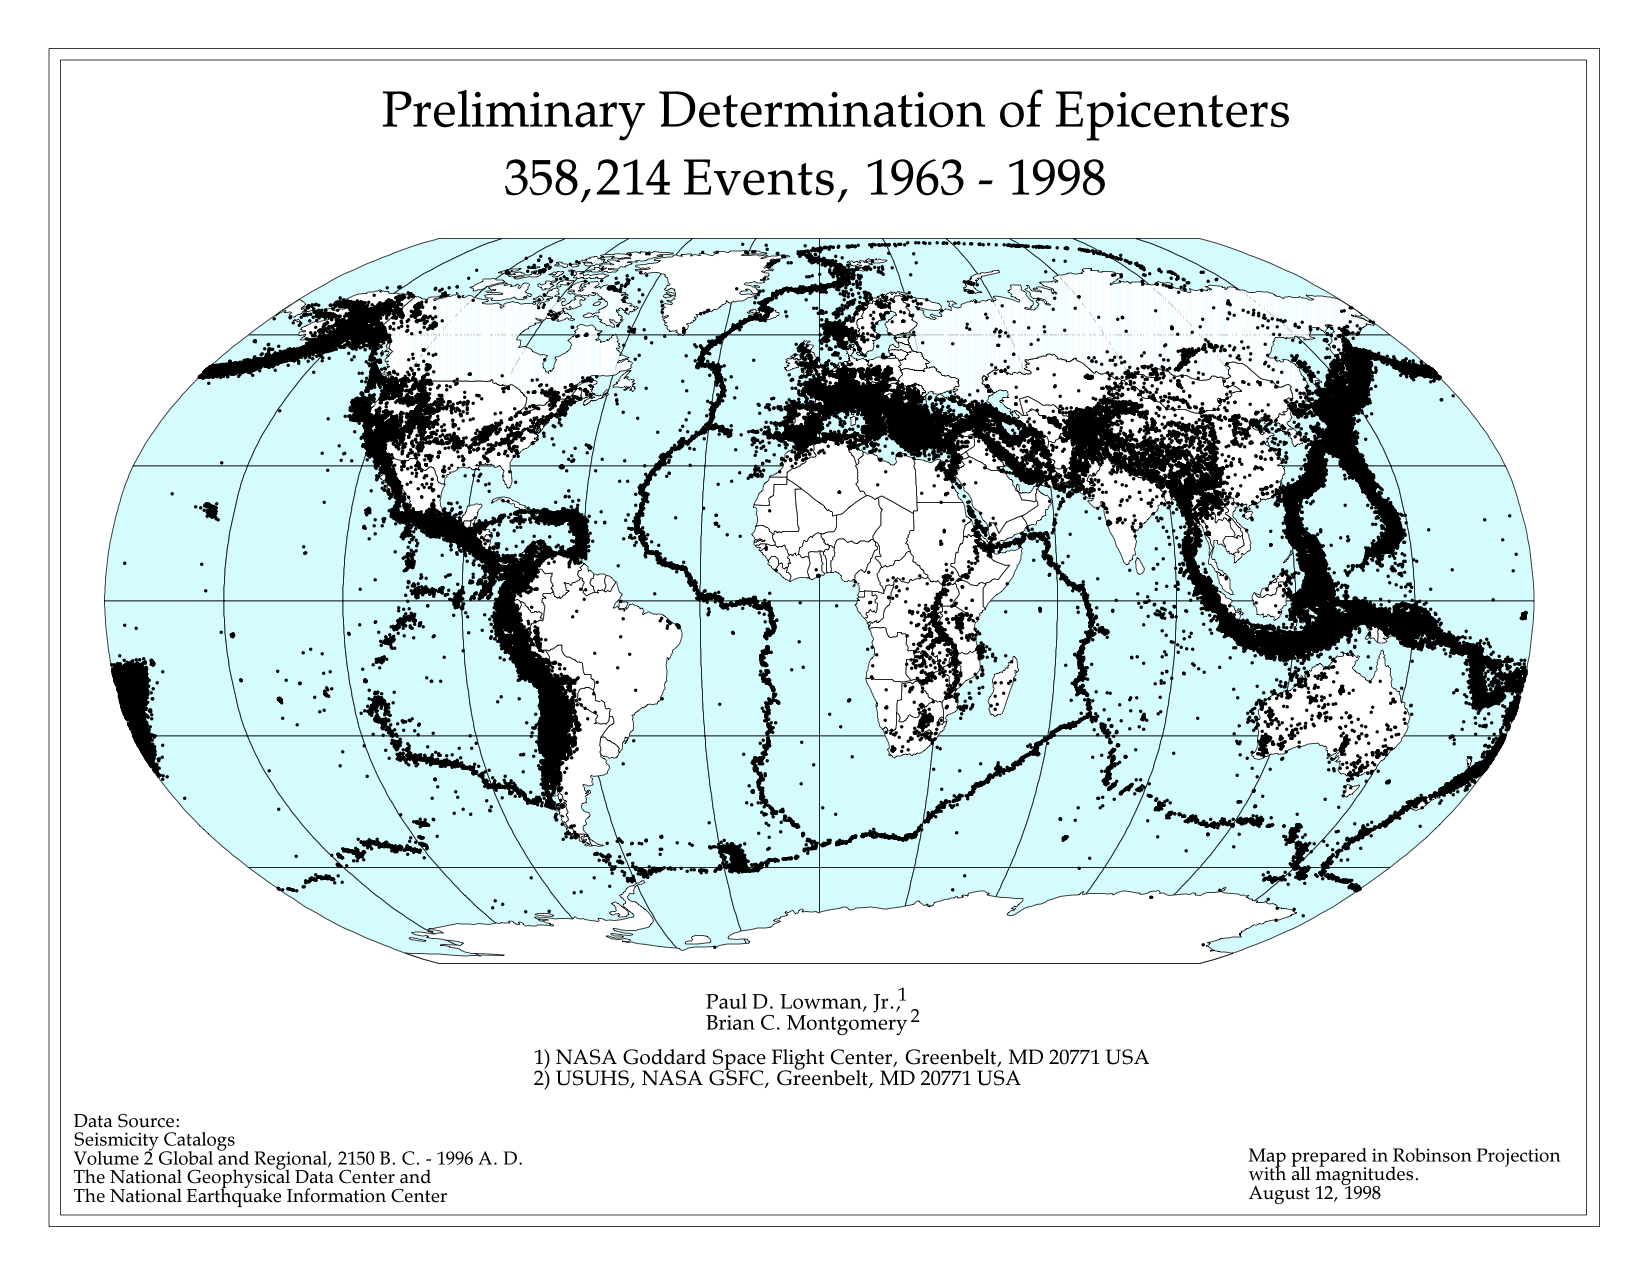
\includegraphics[height=0.95\textheight]{global_pde_mag_all}
   \caption[Mapa Mundial de Epicentros 1963-1998]
   		   {Mapa Mundial de Epicentros 1963-1998 - \citet{lowman_jr_1998}} 
   \label{f:global_epicenters}
\end{figure} 
\end{frame}


%-----------------------------------------------------------------------------
\begin{frame}{Teoria de Placas}
\begin{figure}[H]
   \centering
   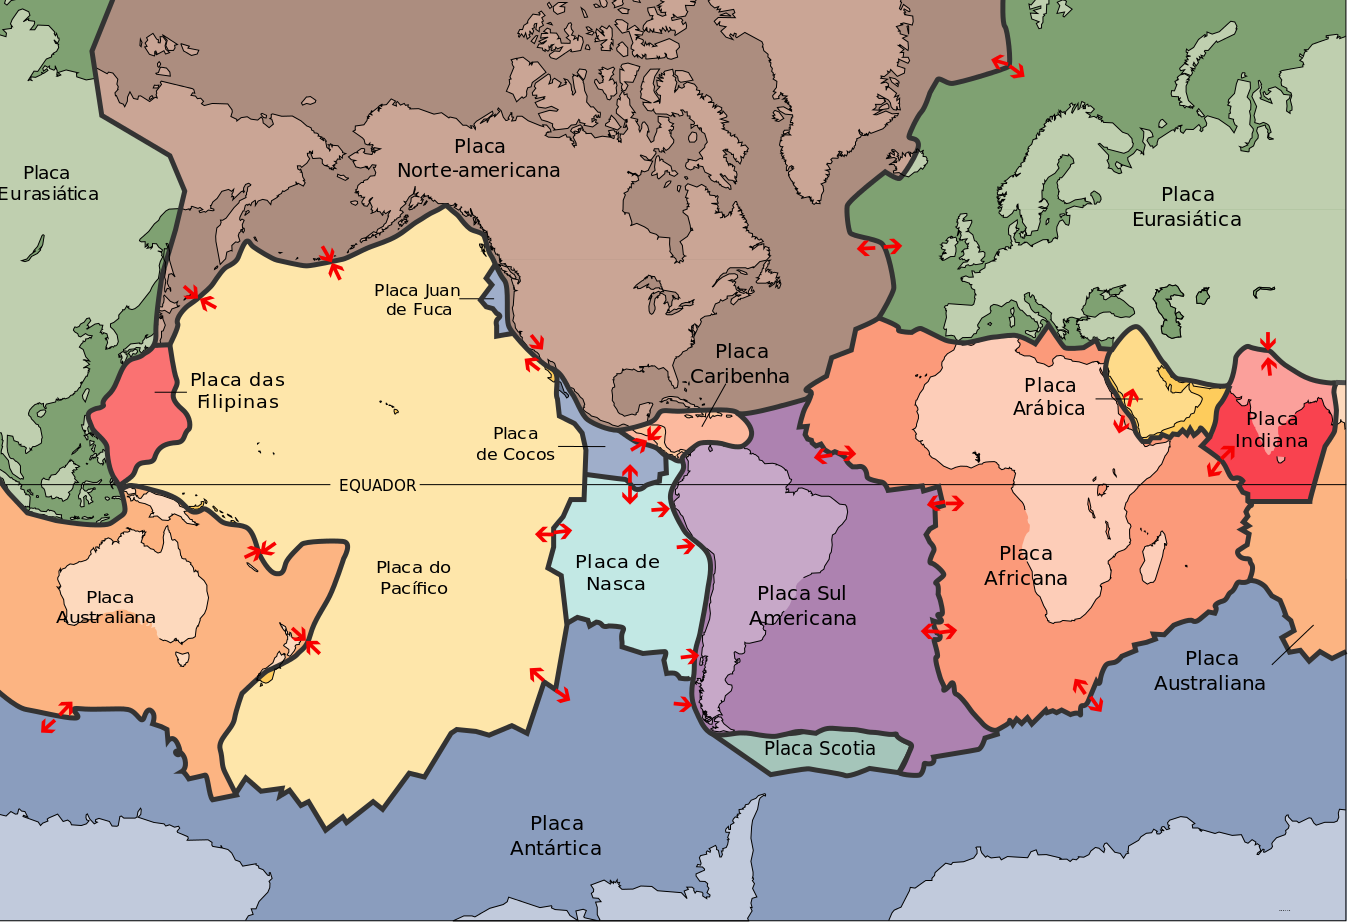
\includegraphics[height=0.95\textheight]{litho_plates_overview}
   \caption[Cartografia das placas litosféricas]
   		   {Cartografia das placas litosféricas - \citet{usgs_plates_1996}} 
   \label{f:plates_overview}
\end{figure} 
\end{frame}



%=============================================================================
\subsection{Sismicidade da América do Sul}
%=============================================================================

%-----------------------------------------------------------------------------
\begin{frame}{Sismicidade da América do Sul}
\begin{figure}[H]
	\centering
	\begin{subfigure}[t]{0.48\textwidth}
	  \centering
	  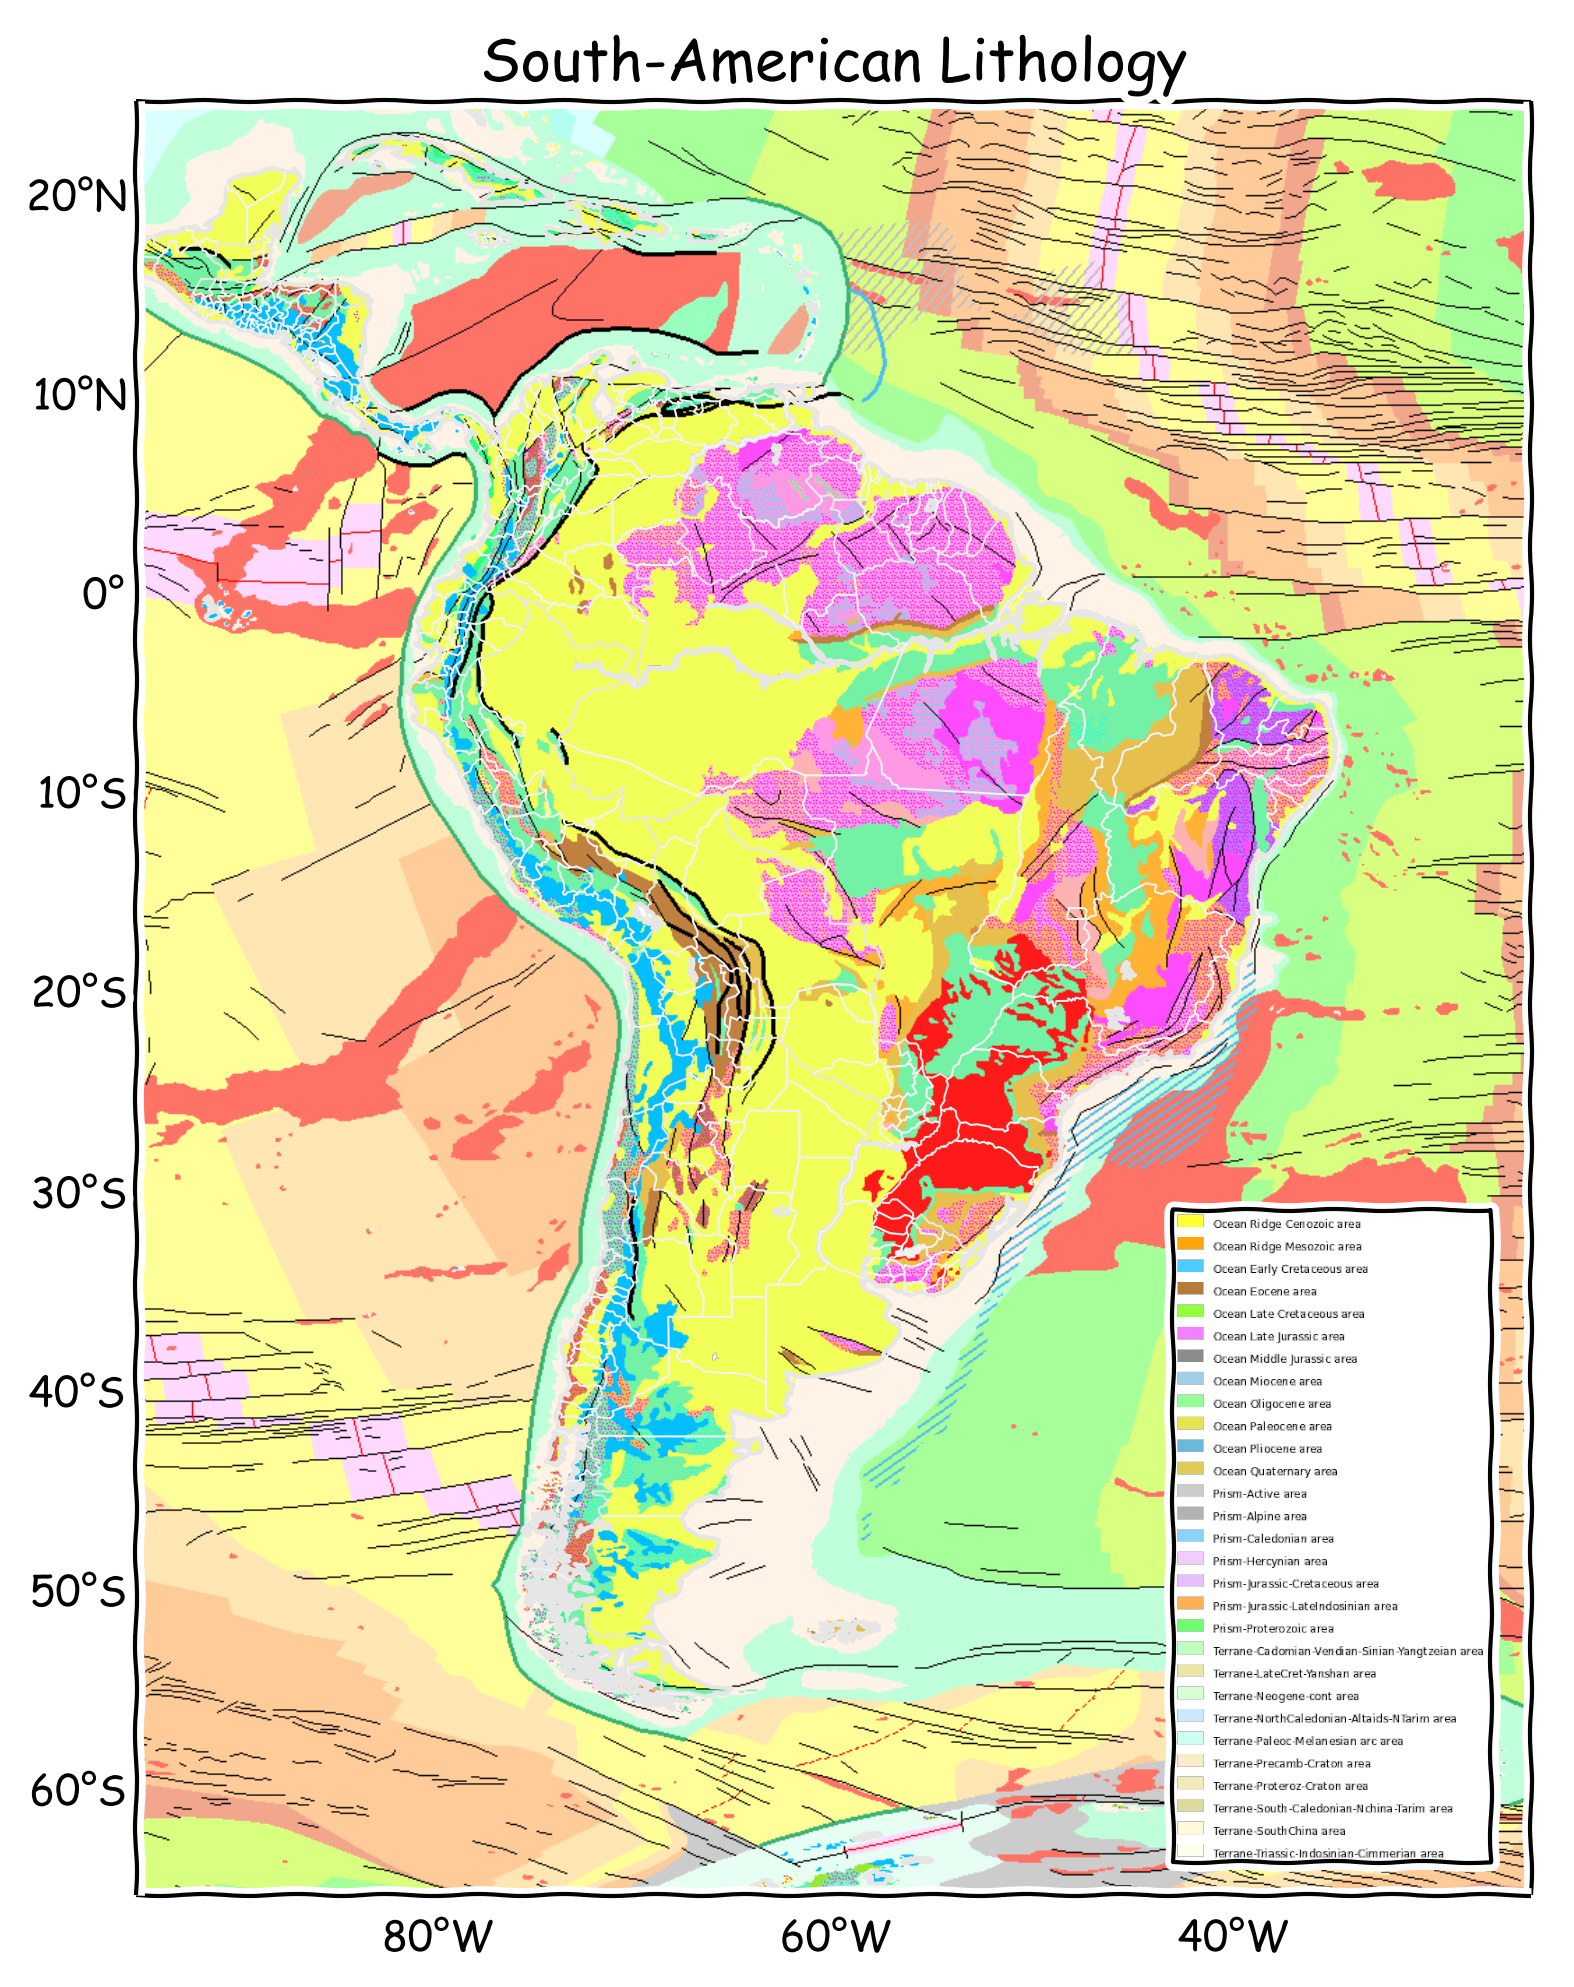
\includegraphics[width=.85\textwidth]{lithology_sa} 
	  \subcaption{Mapa geológico. (\url{http://onegeology.org}).}
	  \label{fig:sa_tec} 
	\end{subfigure}
	\quad %~ %add desired spacing between images, e. g. ~, \quad, \qquad, \hfill etc.
	\begin{subfigure}[t]{0.48\textwidth}
	  \centering
	  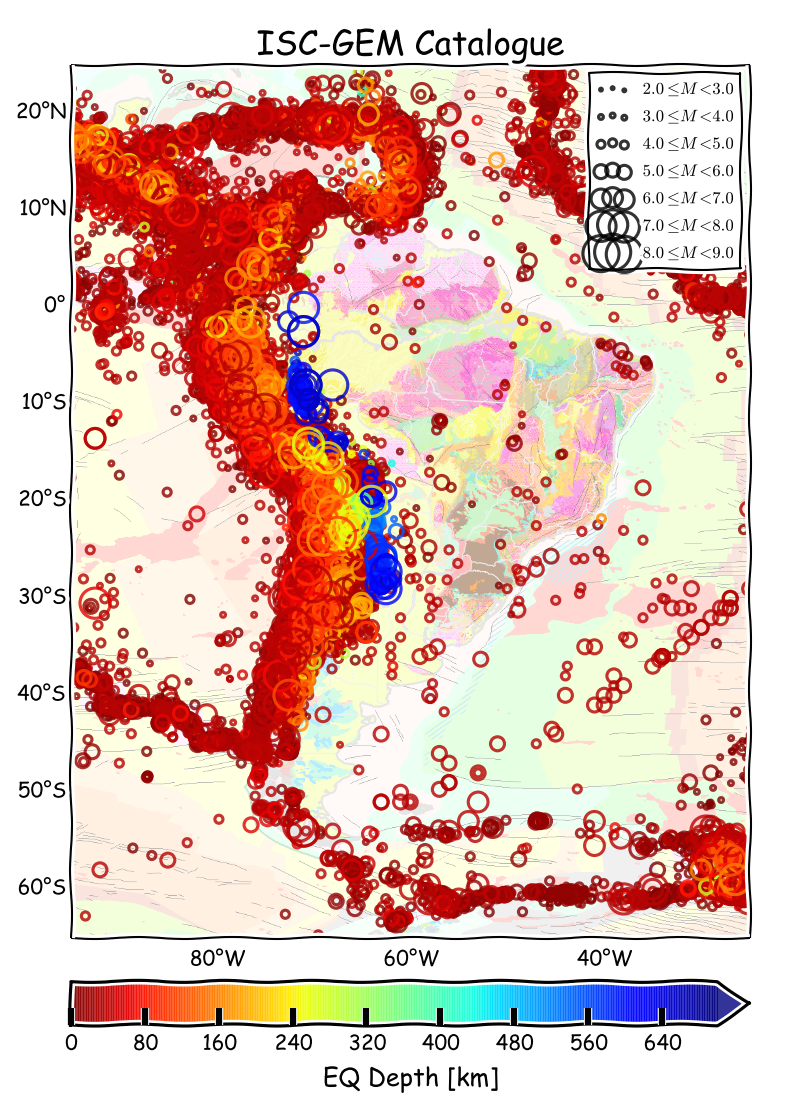
\includegraphics[width=.85\textwidth]{seismicity_sa} 
	  \subcaption{Sismicidade, Catálogo ISC-GEM. 
	  			Geologia: \gls{cgmw} via OneGeology.}
	  \label{fig:sa_seis} 
	\end{subfigure}
	%\caption{Geologia e Sismicidade da América do sul}
	\label{fig:eq_record}
\end{figure}
\end{frame}



%=============================================================================
\subsection{Sismicidade do Brasil}
%=============================================================================

%-----------------------------------------------------------------------------
\begin{frame}{Geologia e Sismicidade do Brasil}
\begin{figure}[H]
	\scriptsize
	\centering
	\begin{subfigure}[t]{0.48\textwidth}
	  \centering
	  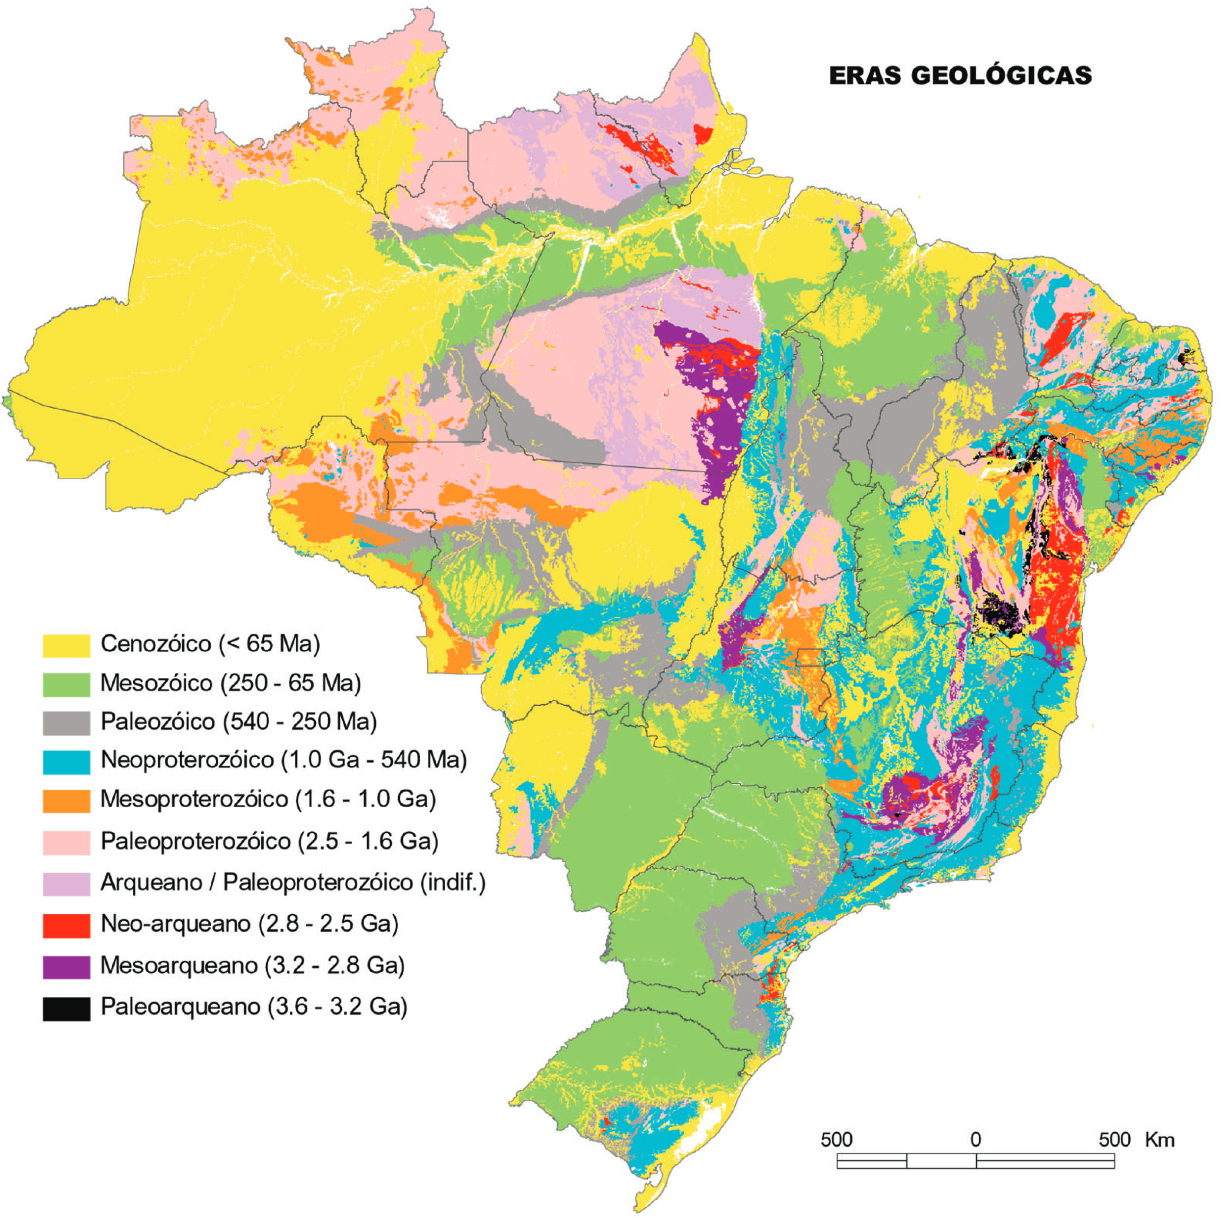
\includegraphics[width=1.0\textwidth]{tectonico_brasil} 
	  \subcaption{Mapa Geológico do Brasil em escala 1:1.000.000.
	  \citet{bizzi_2003}}
	  \label{fig:br_tec} 
	\end{subfigure}
	\begin{subfigure}[t]{0.48\textwidth}
	  \centering
	  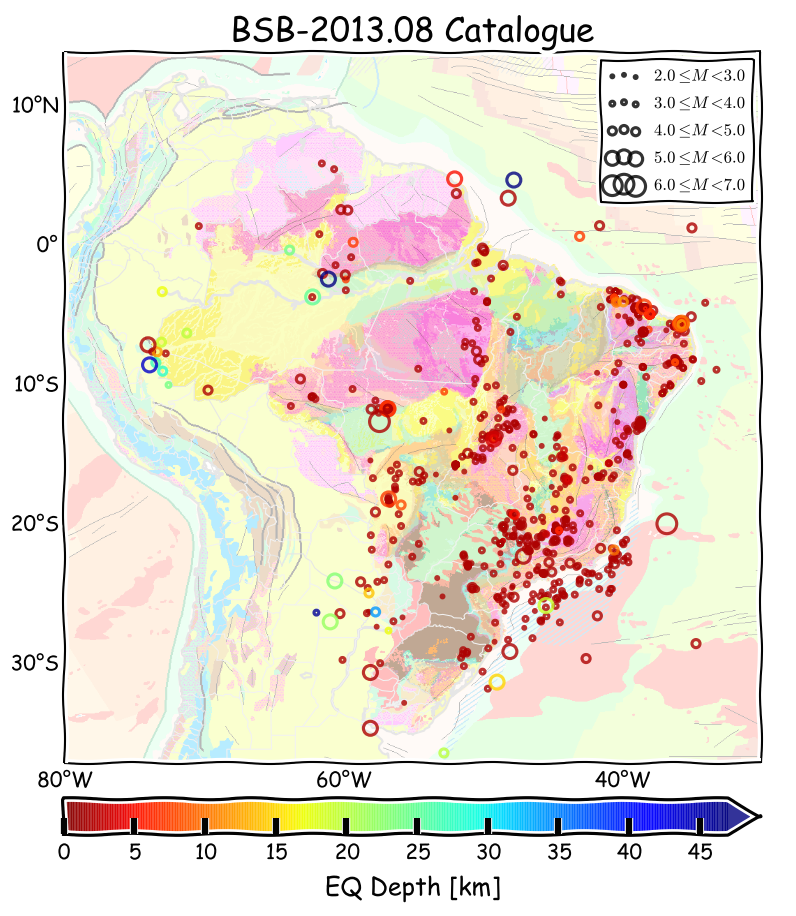
\includegraphics[width=1.0\textwidth]{seismicity_br} 
	  \subcaption{Sismicidade do Brasil. Catálogo \gls{bsb2013}.}
	  \label{fig:br_seis} 
	\end{subfigure}
	%\caption{Geologia e Sismicidade do Brasil}
	\label{fig:eq_record}
\end{figure}
\end{frame}



%=============================================================================
\section{O problema}
%=============================================================================
%=============================================================================
\subsection{Cálculo de ameaça sísmica}
%=============================================================================
%-----------------------------------------------------------------------------
\begin{frame}{Cálculo da ameaça sísmica: fluxo de trabalho}
\begin{figure}[H]
	\centering
	\begin{tabular}{l}
	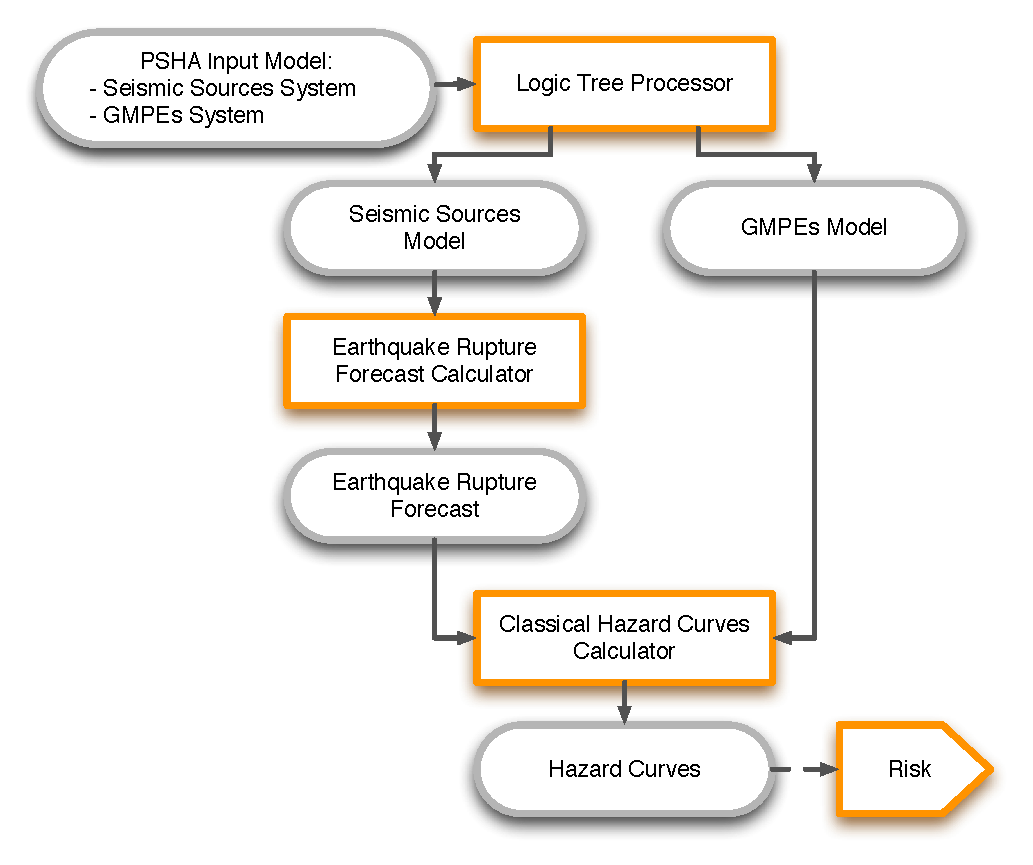
\includegraphics[height=0.90\textheight]{classical_psha_workflow}
	\end{tabular}
	\caption{Fluxo de trabalho clássico para a \gls{psha} \citep{crowley_2013}.}
\label{fig:classical_psha}
\end{figure}
\end{frame}



%=============================================================================
\subsection{Ferramentas}
%=============================================================================
%-----------------------------------------------------------------------------
\begin{frame}{Openquake}
\begin{figure}[!h]
  \centering
  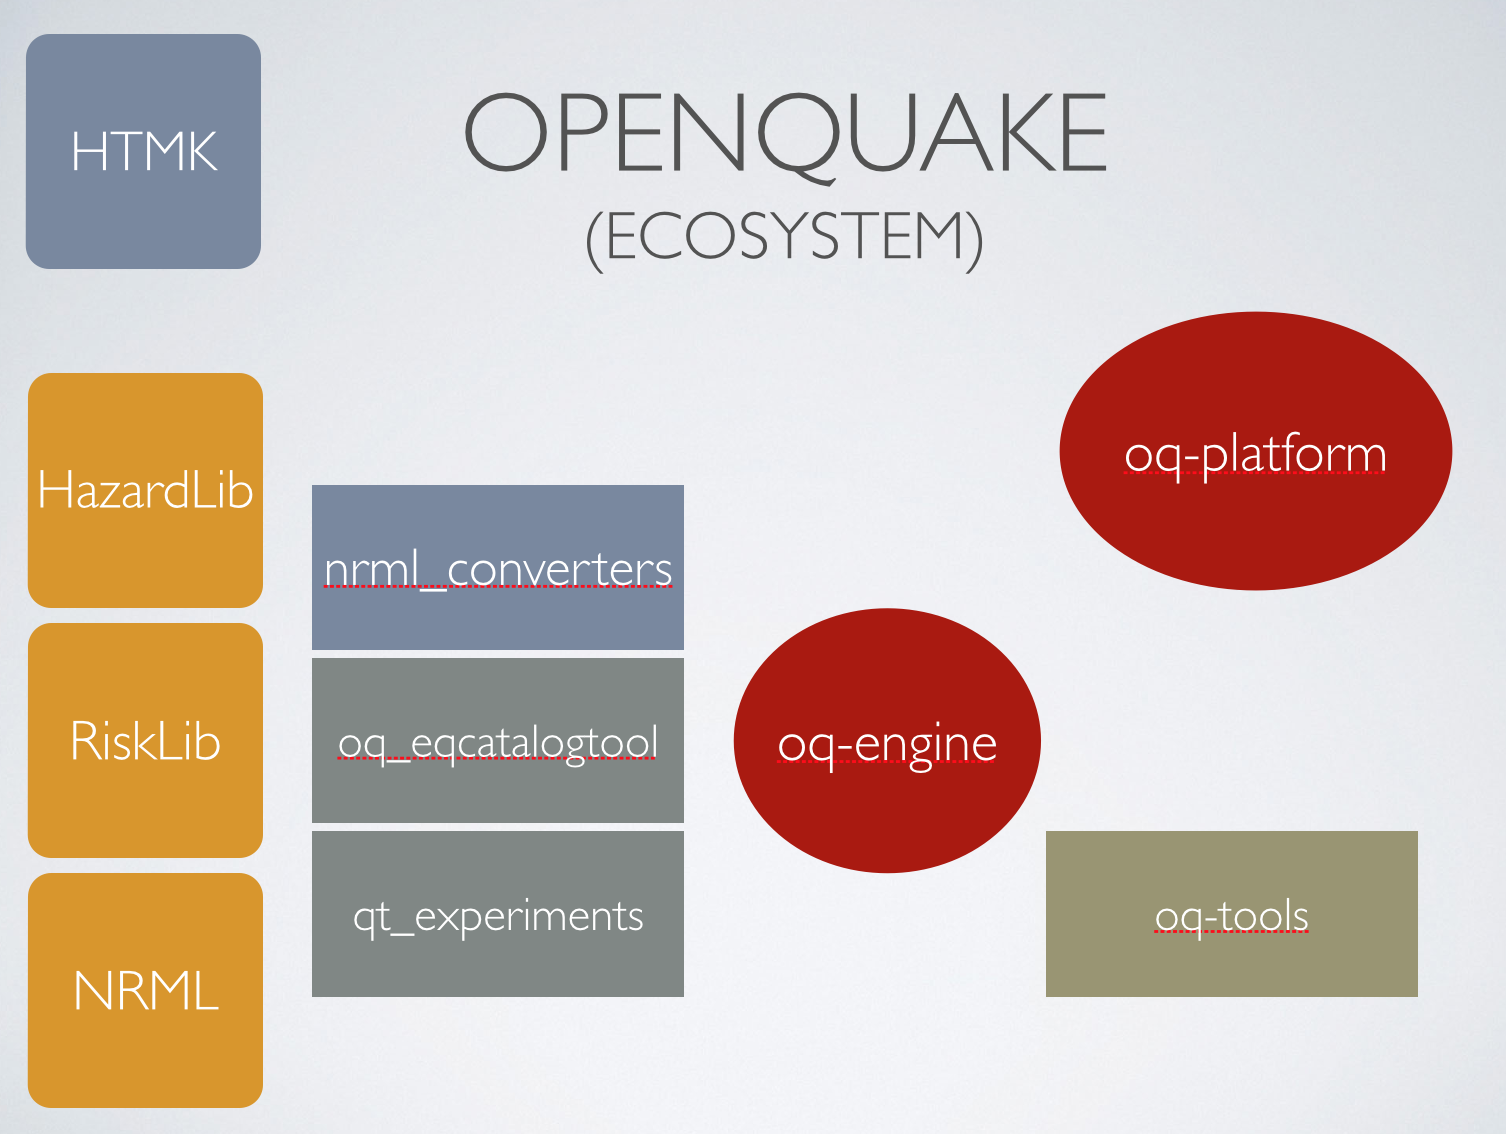
\includegraphics[height=.90\textheight]{oq_ecosystem} 
  \caption{Ecossistema de módulos, bibliotecas e utilitários do OpenQuake}
  \label{fig:oq} 
\end{figure}
\end{frame}



%=============================================================================
\subsection{Resultados Anteriores}
%=============================================================================
%-----------------------------------------------------------------------------
\begin{frame}{GSHAP: Ameaça}
\begin{figure}[H]
  \centering
  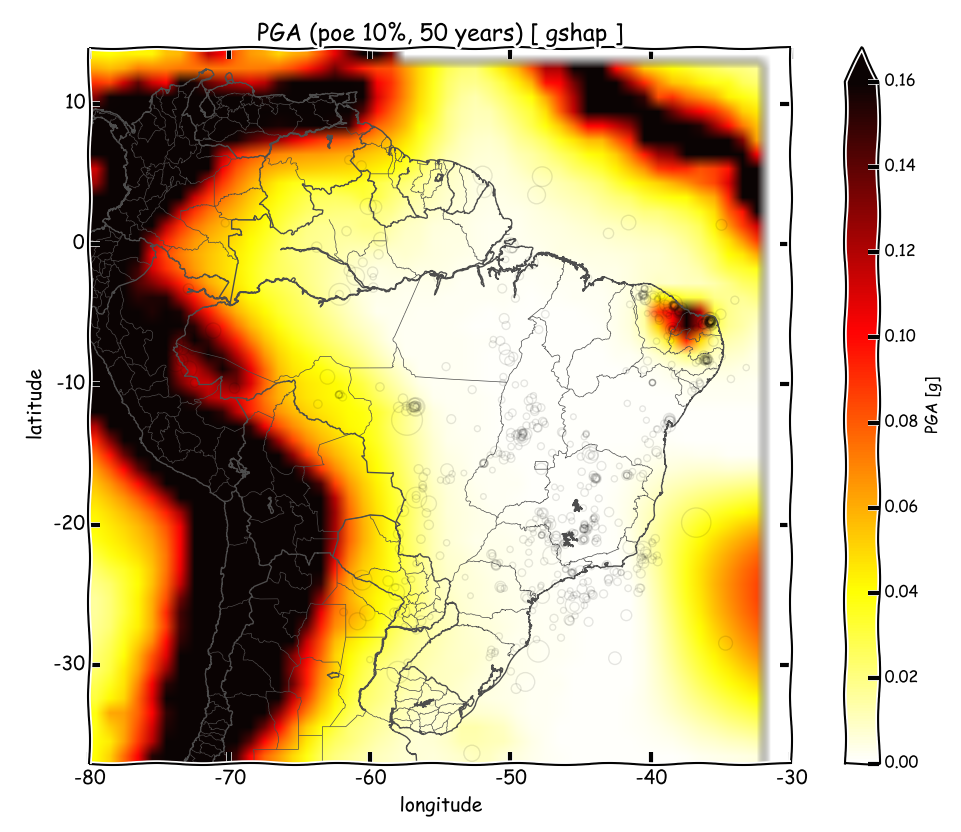
\includegraphics[height=.95\textheight]{pga_gshap} 
  \caption{Resultado do GSHAP para o Brasil: \gls{PGA} (10\%/50anos) em unidades de $g$}
  \label{fig:gshap} 
\end{figure}
\end{frame}


%-----------------------------------------------------------------------------
\begin{frame}{Dourado2014: Zoneamento (Cornell \& McGuire)}
\begin{figure}[H]
  \centering
  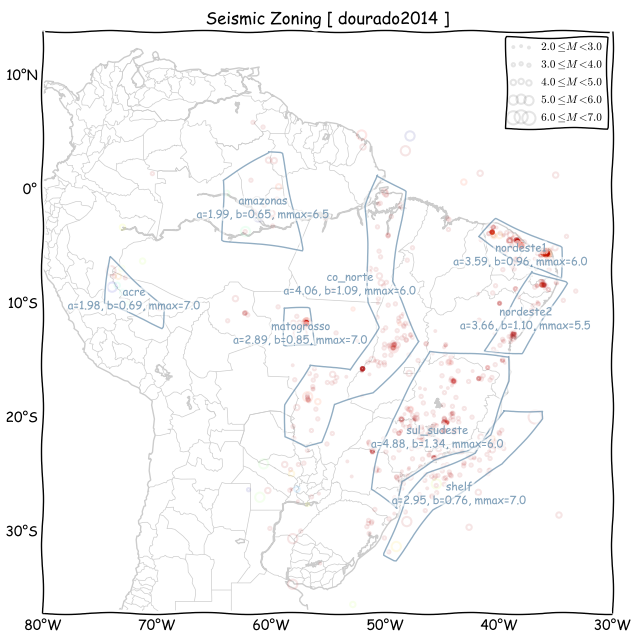
\includegraphics[height=.93\textheight]{a_dourado} 
  \caption{Zoneamento sísmico e caracterização das zonas sísmicas por \citep{dourado_2014}.
  Os valores para a magnitude mínima foram de 3.0}
  \label{fig:a_dourado} 
\end{figure}
\end{frame}


%-----------------------------------------------------------------------------
\begin{frame}{Dourado2014: Ameaça}
\begin{figure}[H]
  \centering
  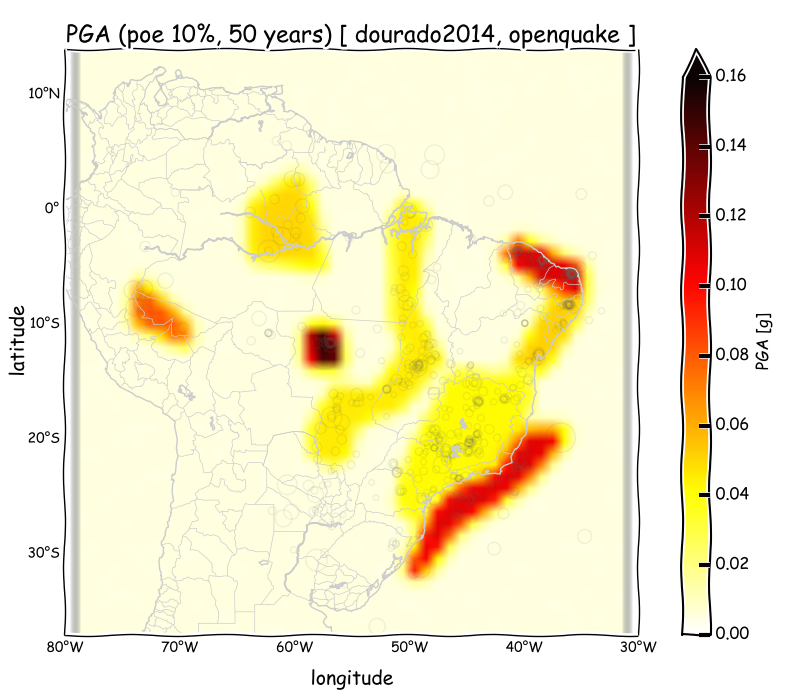
\includegraphics[height=.95\textheight]{pga_dourado_oq} 
  \caption{Mapa de ameaça sísmica, PGA(poe 0.1, 50y)[Dourado, 20014] OpenQuake-Engine }
  \label{fig:pga_dourado_oq} 
\end{figure}
\end{frame}




%=============================================================================
\section{Dados}
%=============================================================================
%=============================================================================
\subsection{Análise exploratória}
%=============================================================================



%-----------------------------------------------------------------------------
\begin{frame}{Distribuições de Frequência e Magnitude}
\begin{figure}[H]
   \centering
   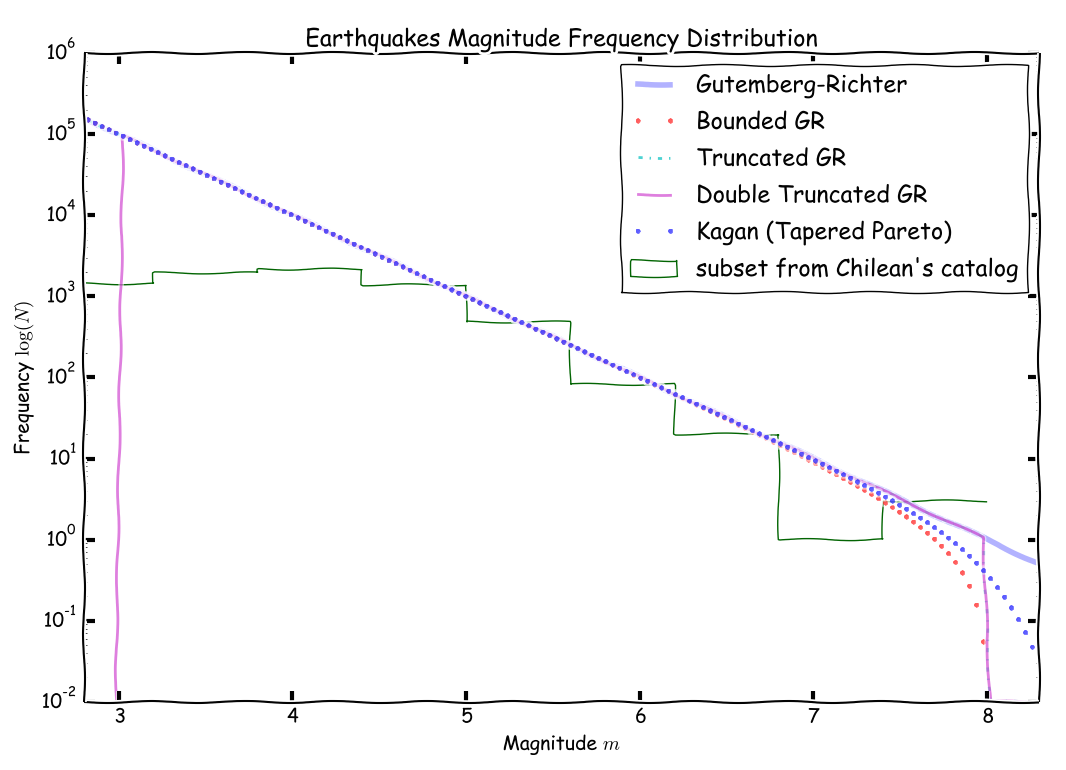
\includegraphics[height=0.90\textheight]{mfd}
   \caption[Distribuições de frequência e magnitude]
   		   {Distribuições de frequência e magnitude} 
   \label{f:mfd}
\end{figure} 
\end{frame}



%-----------------------------------------------------------------------------
\begin{frame}{MFD: ISC-GEM e BSB2013.08}
\begin{figure}[H]
   \centering
   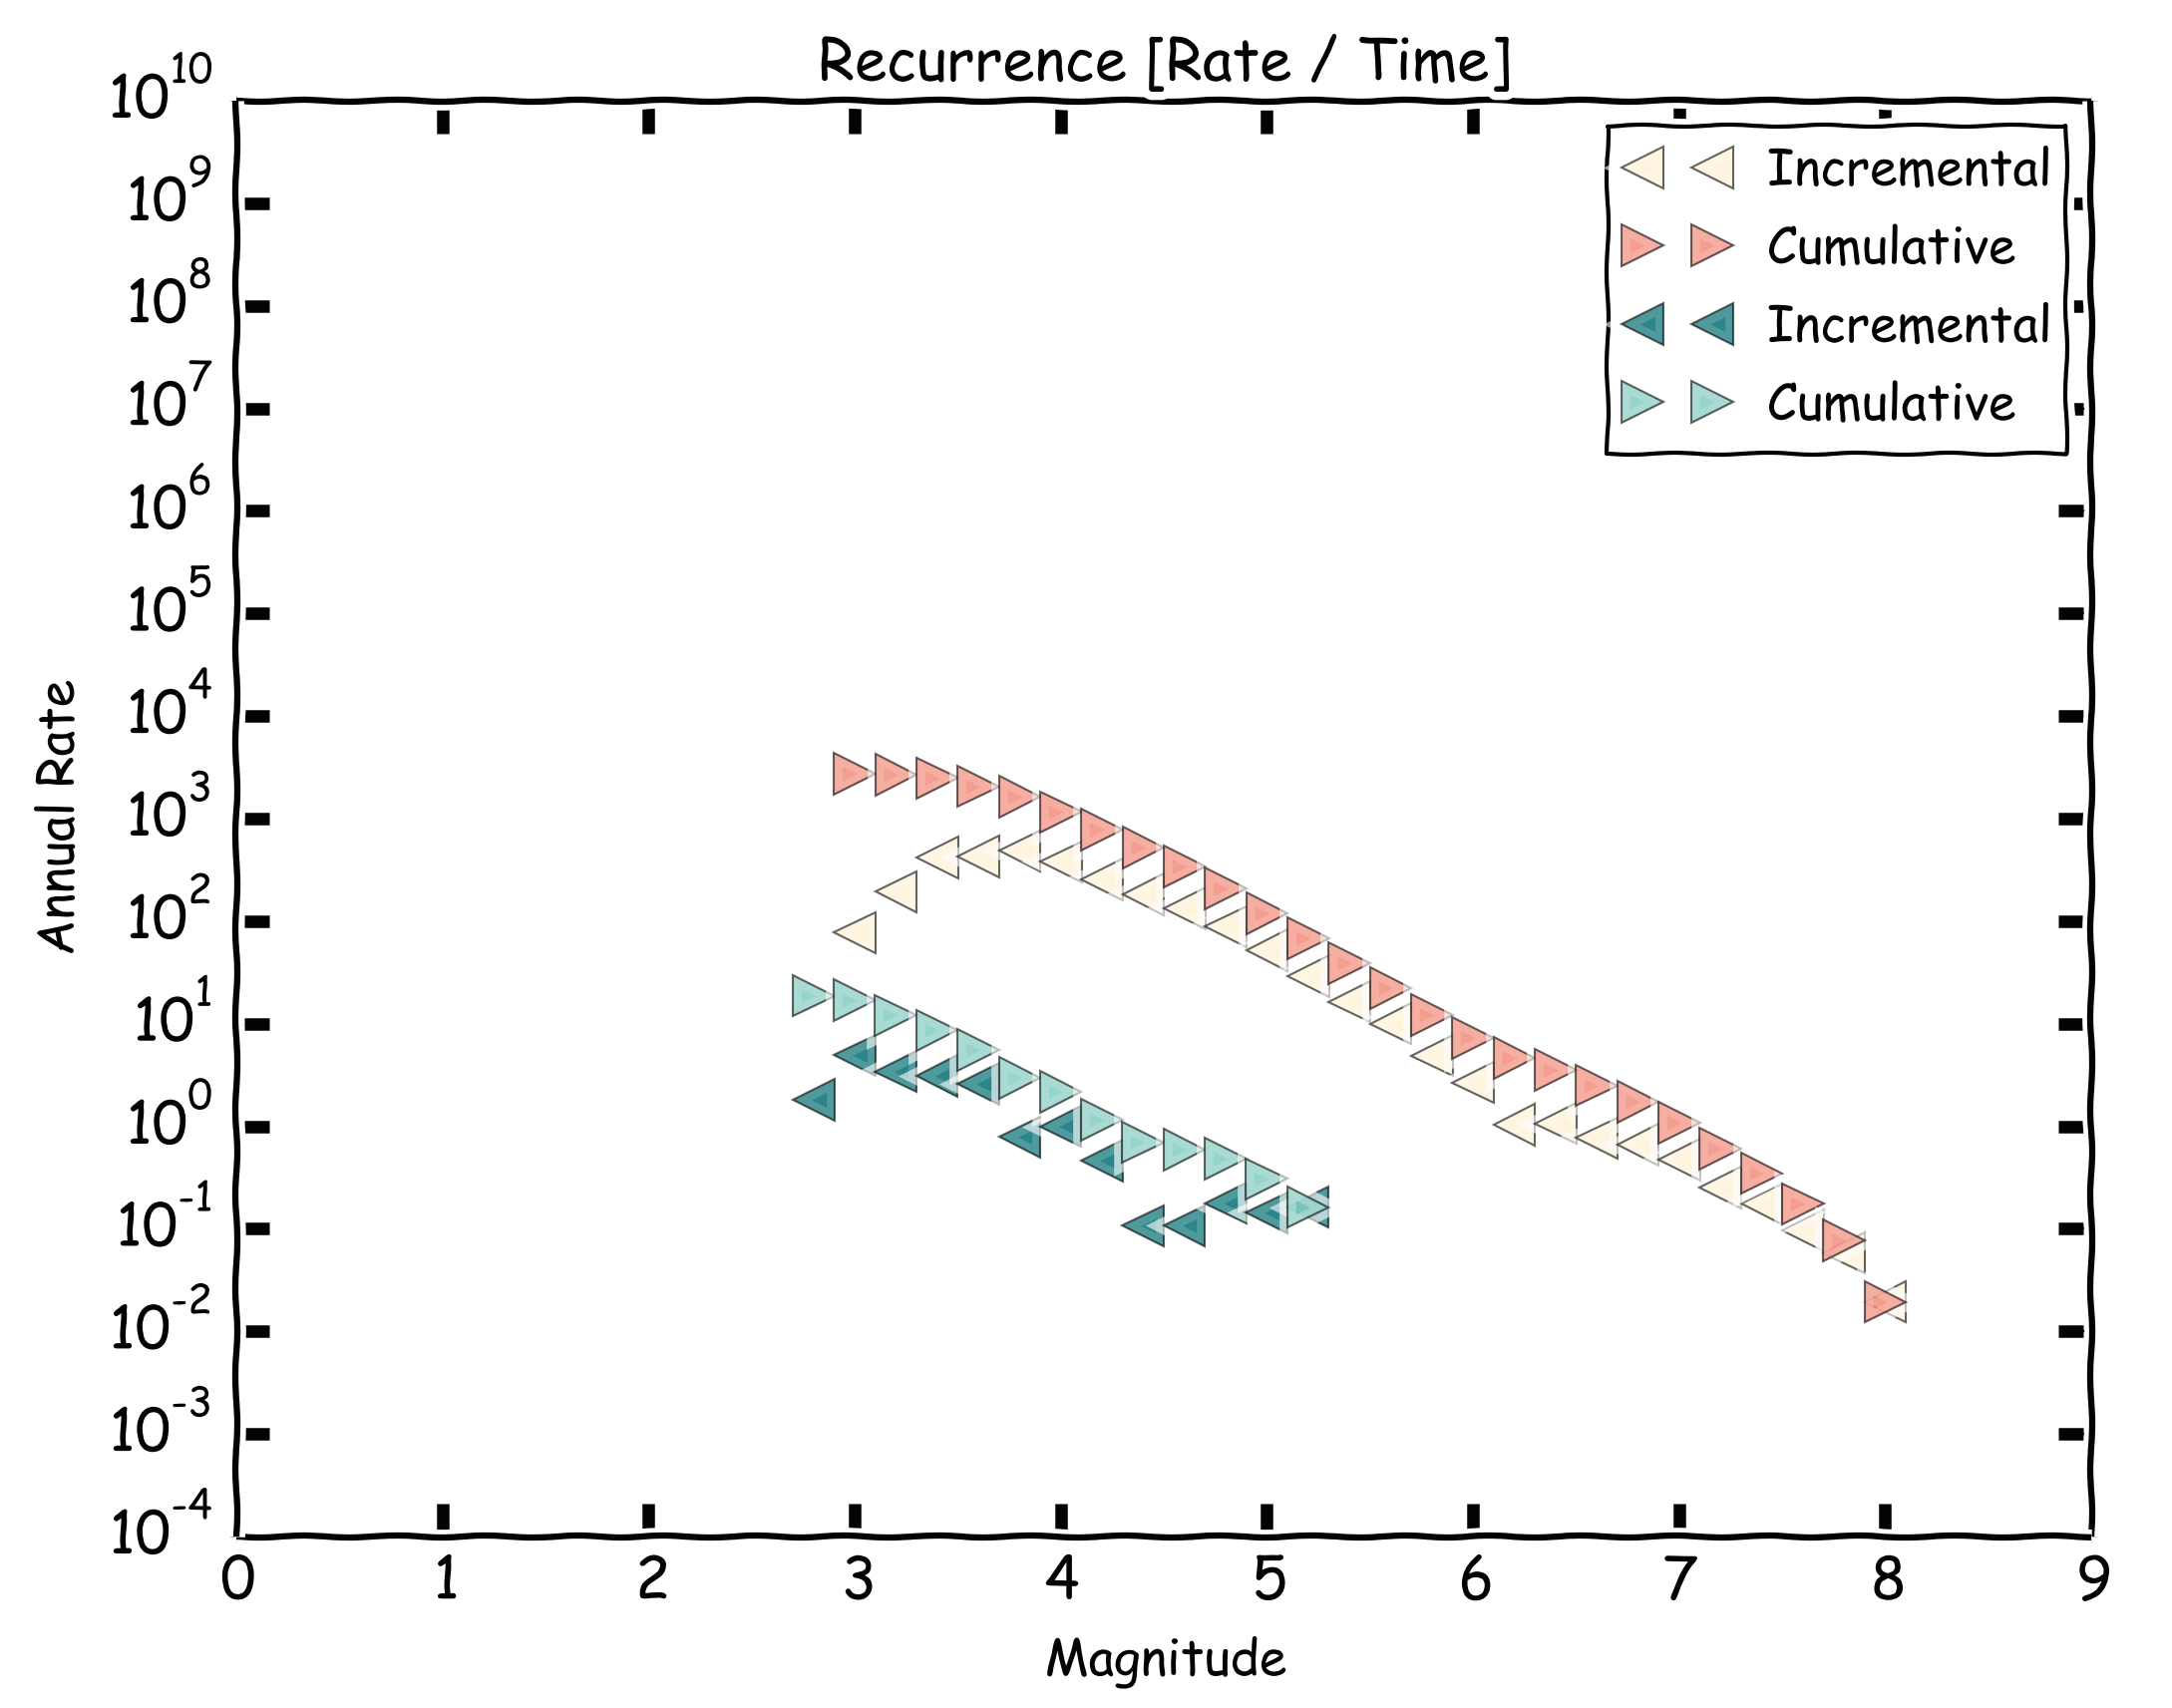
\includegraphics[height=0.90\textheight]{occurrence}
   \caption[Distribuição incremental e cumulativa de frequência e magnitude dos sismos presentes no catálogo ISC-GEM
   para a América do Sul unido com o \gls{bsb2013}]
   {Distribuição incremental e cumulativa de frequência e magnitude dos sismos presentes no catálogo ISC-GEM
   para a América do Sul unido com o \gls{bsb2013}} 
   \label{f:occurrence}
\end{figure} 
\end{frame}



%-----------------------------------------------------------------------------
\begin{frame}{Taxa de sismicidade}
\begin{figure}[H]
	\centering
	\begin{subfigure}[t]{0.48\textwidth}
	  	\centering
		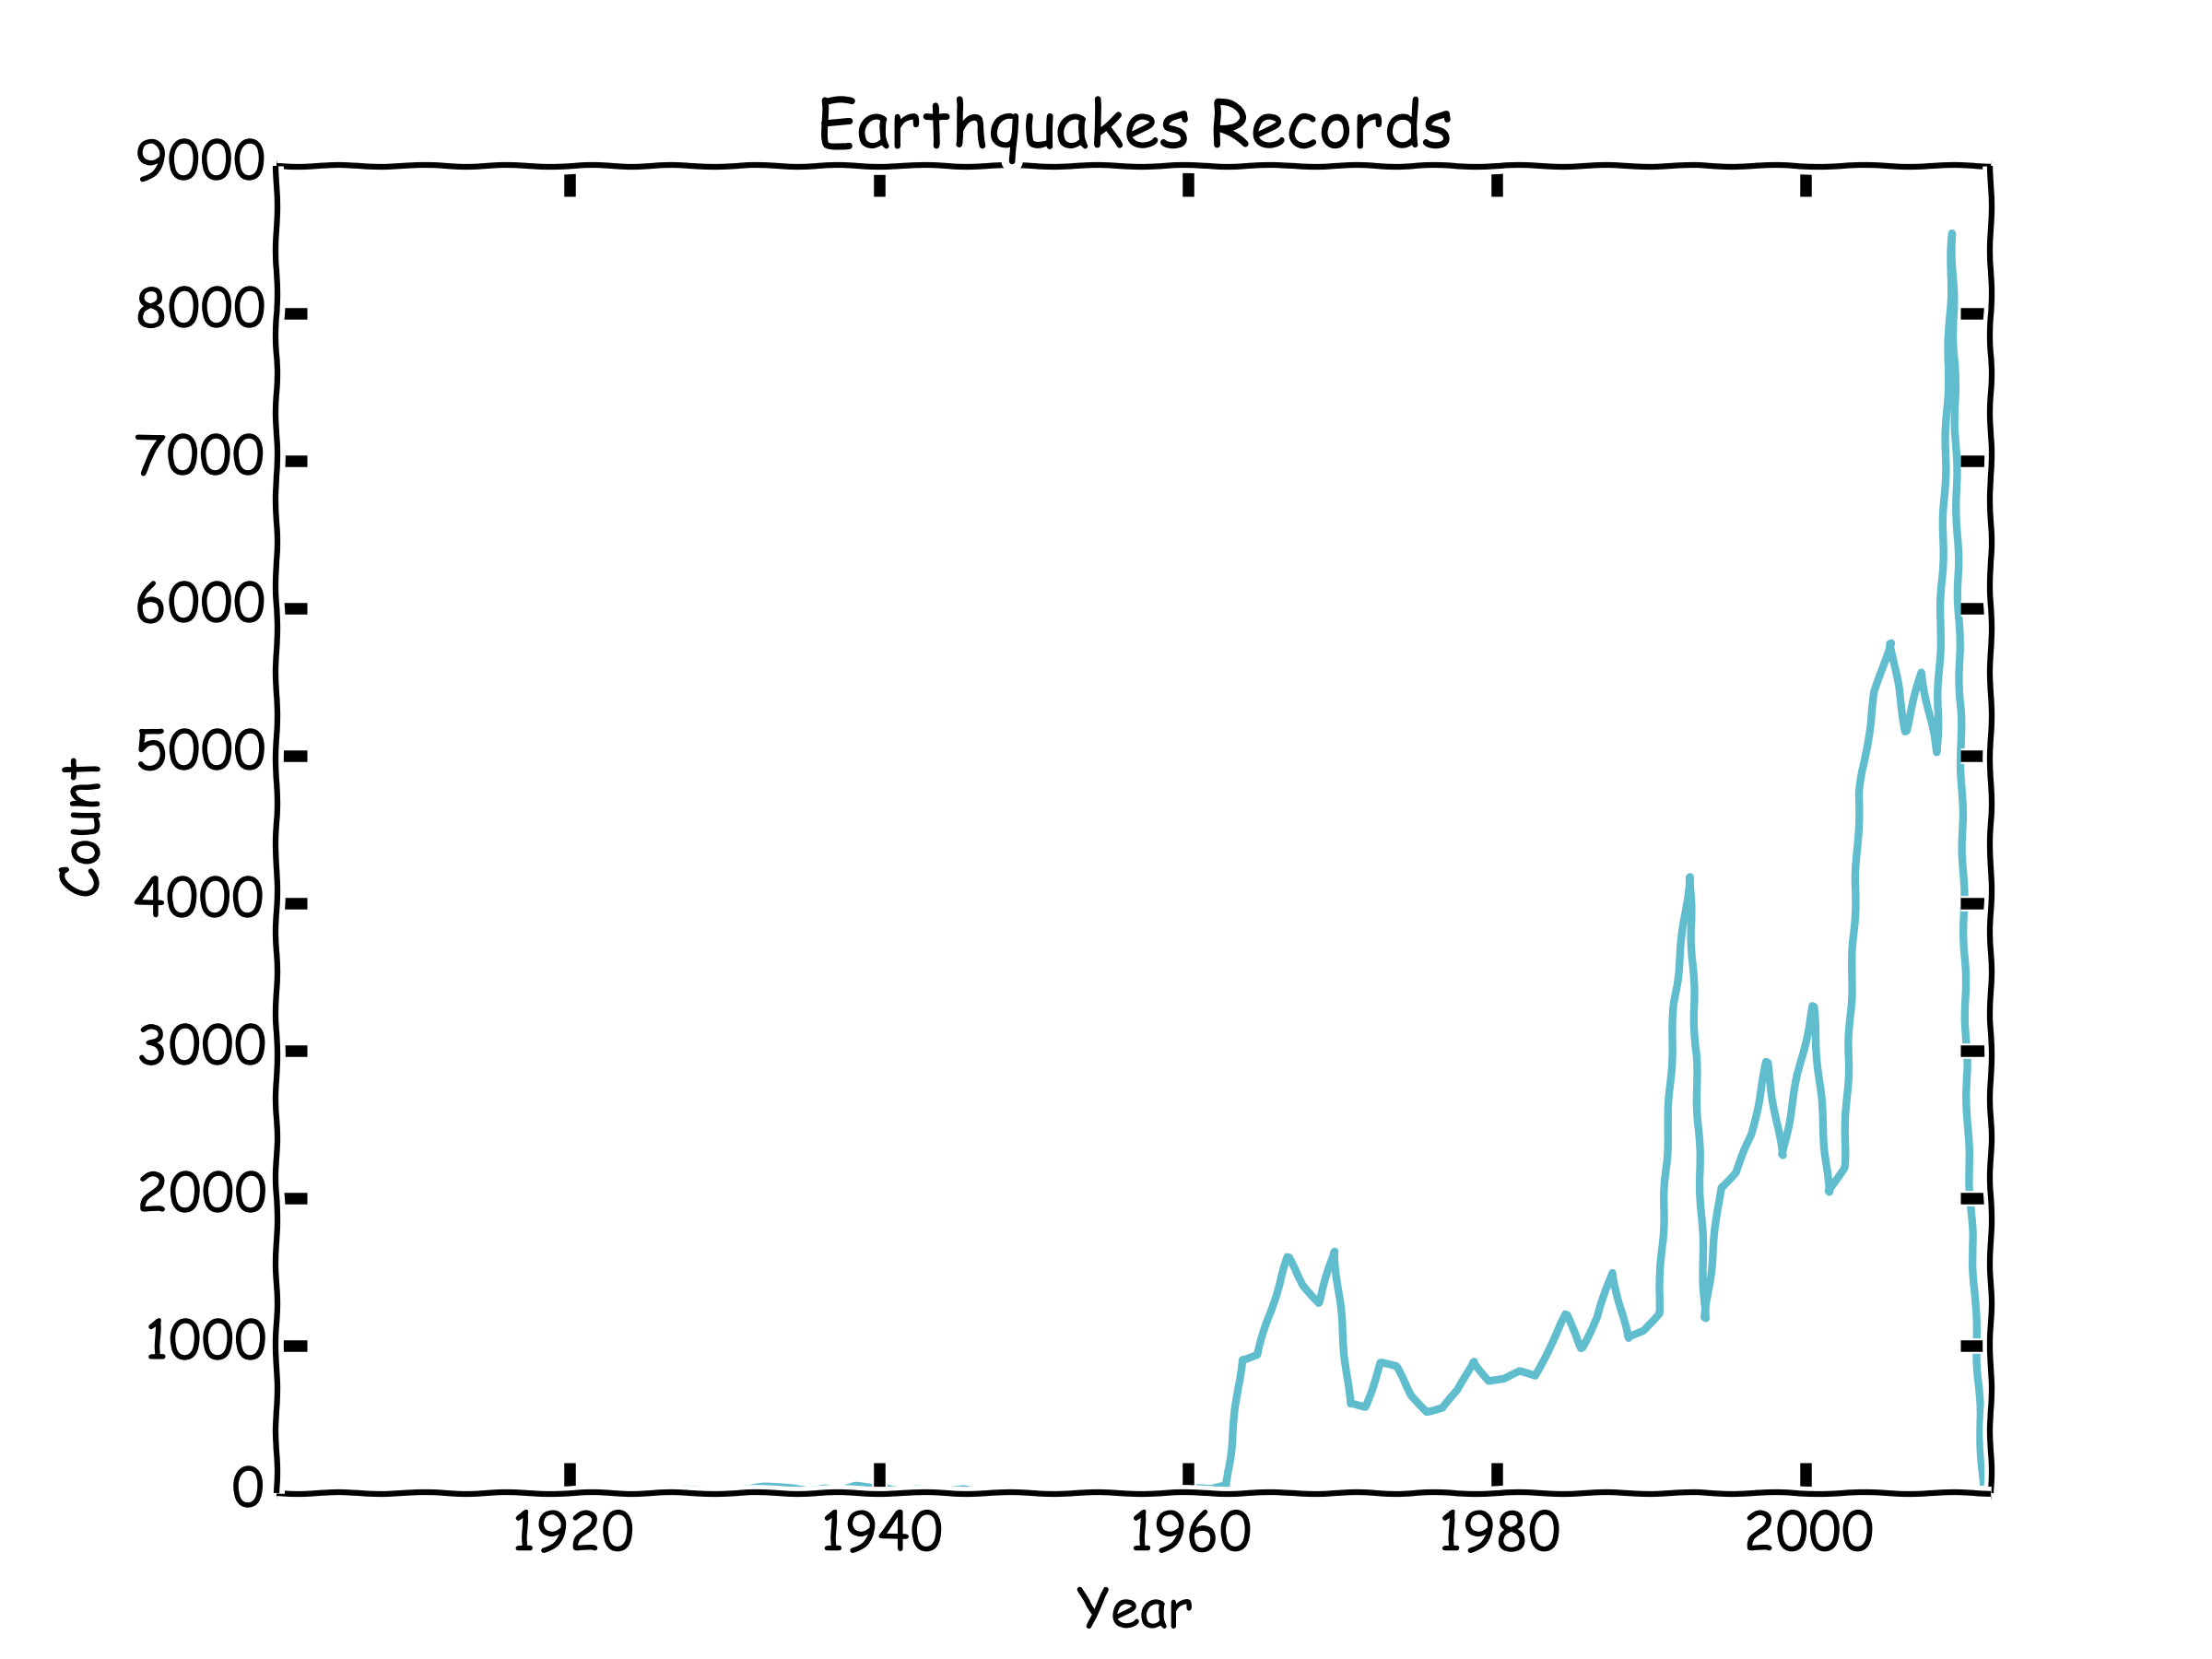
\includegraphics[width=1.0\textwidth]{hmtk_sa3_rate}
		\subcaption{Número de tremores registrados por ano, \gls{iscgem}}
		\label{fig:sa_eq_record}
	\end{subfigure}%
	\quad %~ %add desired spacing between images, e. g. ~, \quad, \qquad, \hfill etc.
	\begin{subfigure}[t]{0.48\textwidth}
	  	\centering
		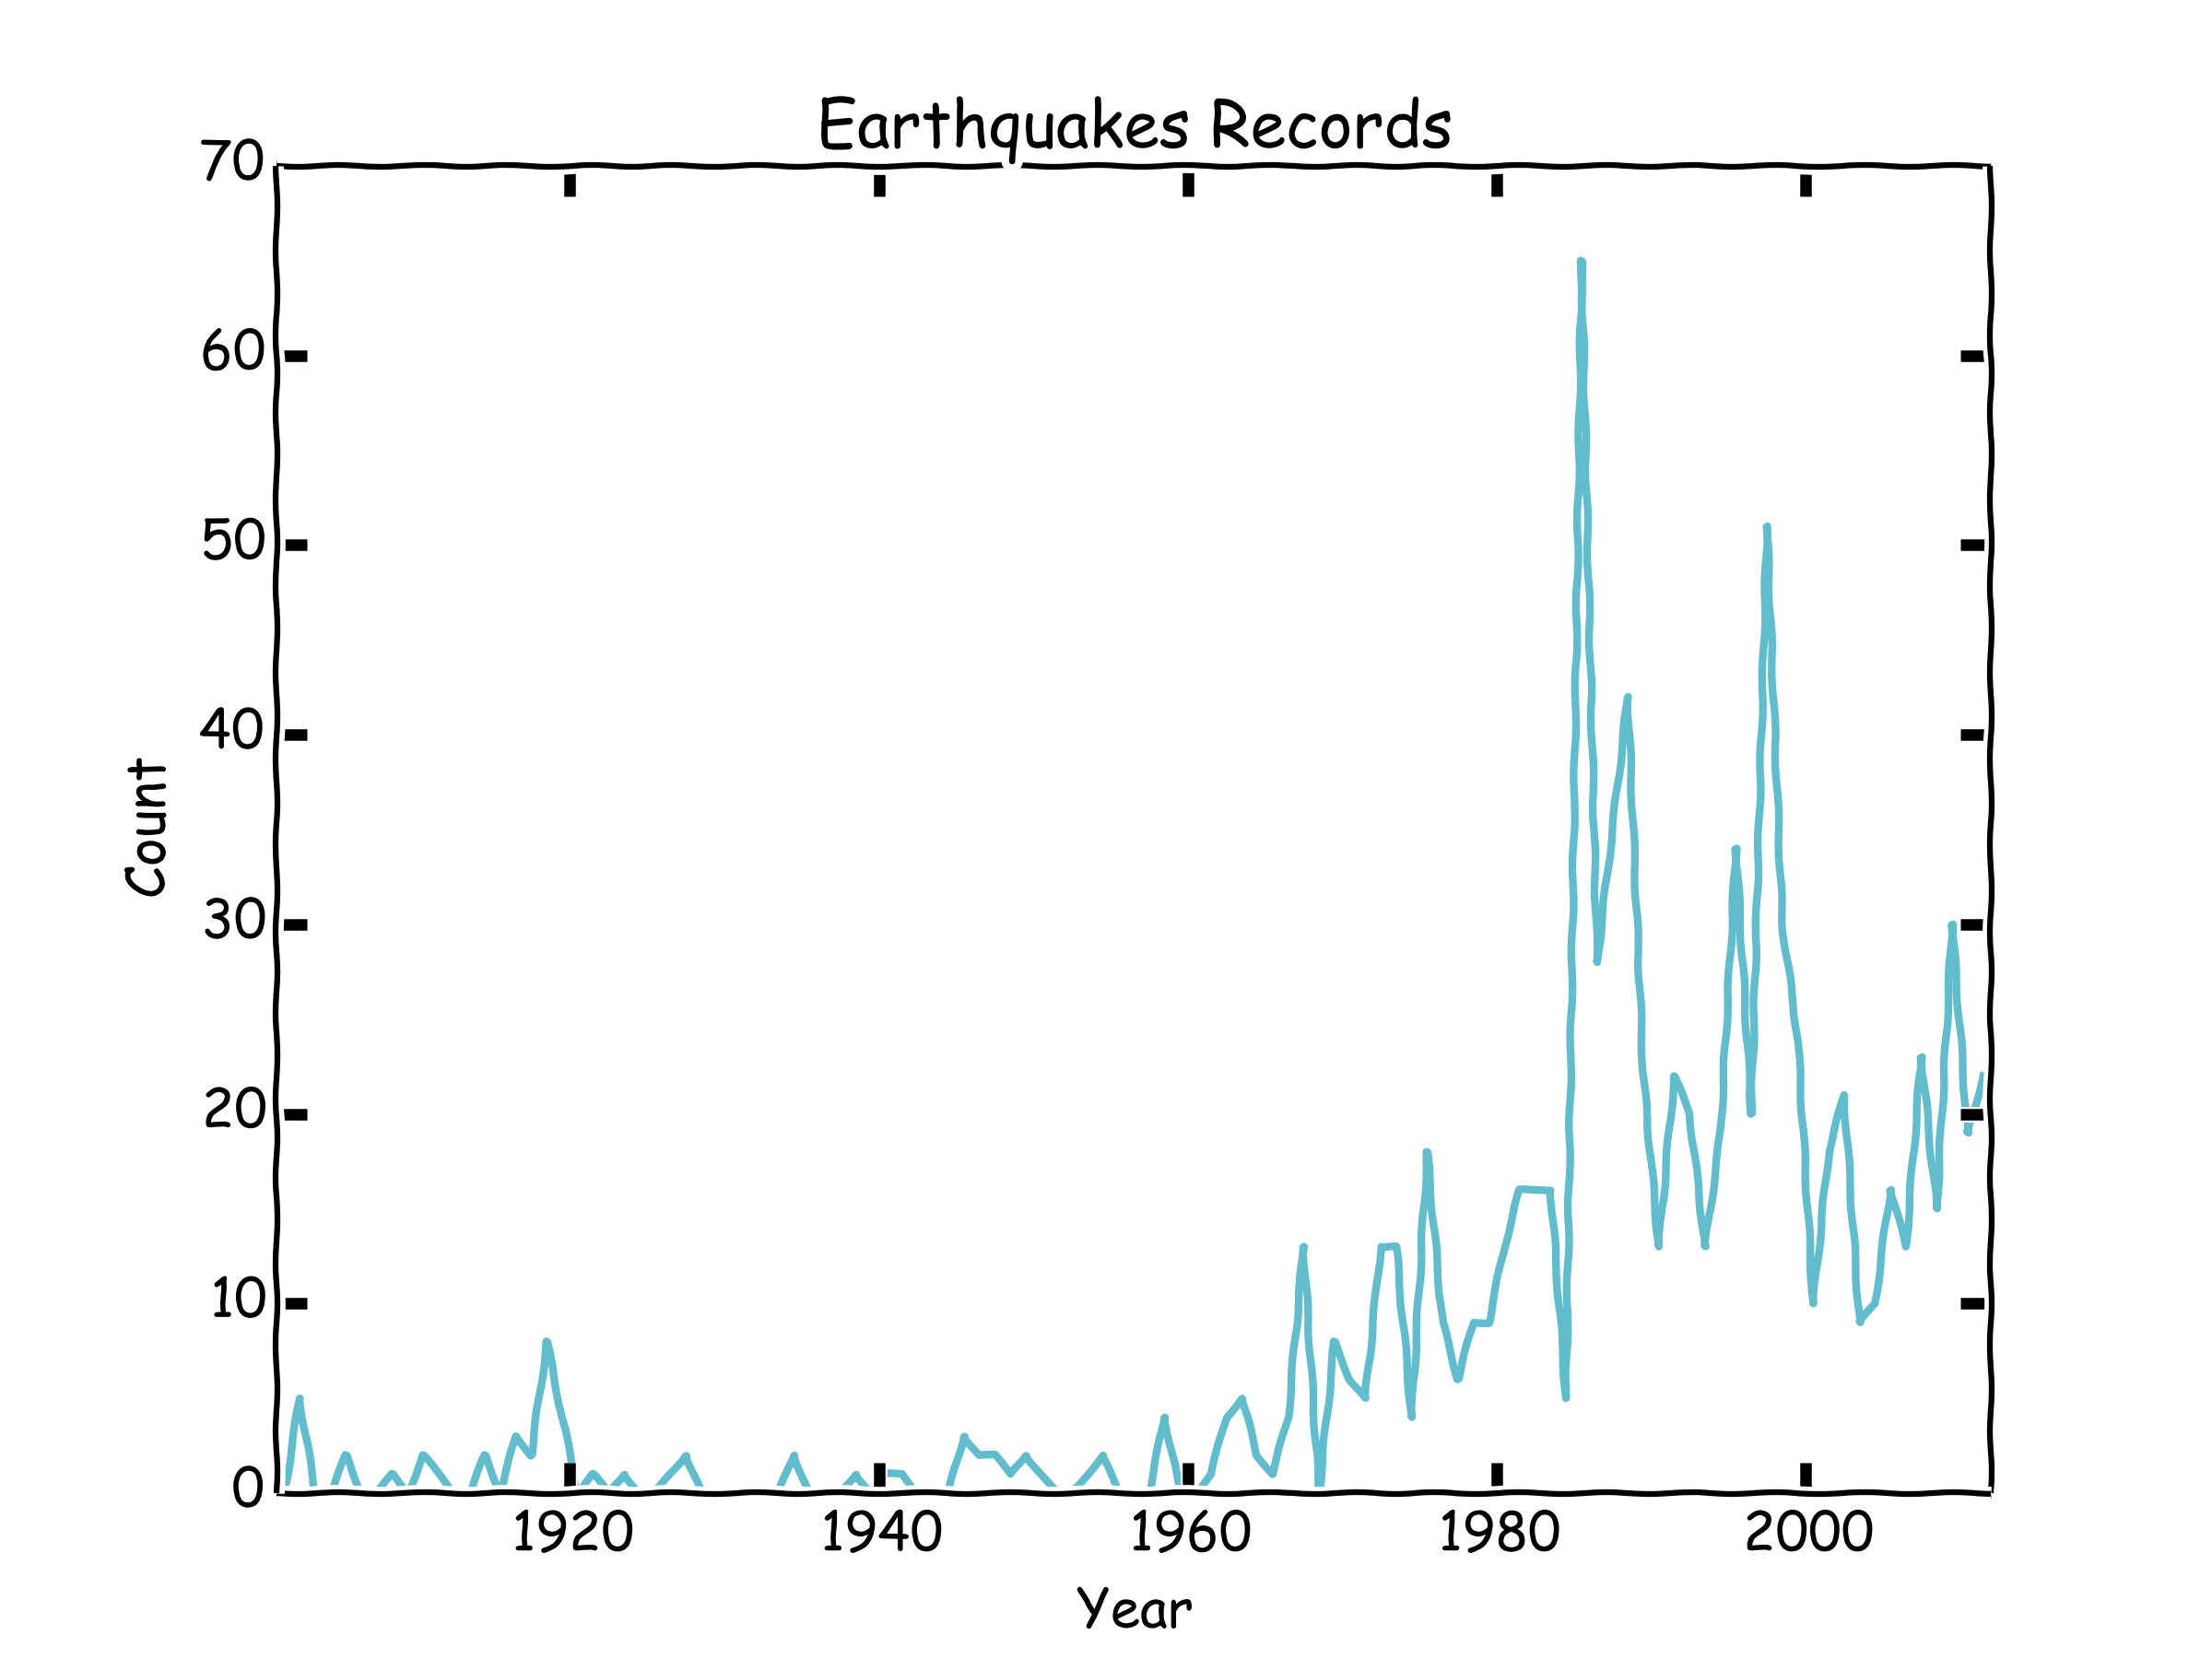
\includegraphics[width=1.0\textwidth]{hmtk_bsb2013_rate}
		\subcaption{Número de tremores registrados por ano, \gls{bsb2013}}
		\label{fig:br_eq_record}
    \end{subfigure}%
	\caption{Número de tremores registrados por ano após 1900}
	\label{fig:eq_record}
\end{figure}
\end{frame}



%-----------------------------------------------------------------------------
\begin{frame}{Distribuição Temporal de Magnitudes: \gls*{iscgem}}
\begin{figure}[H]
	\centering
	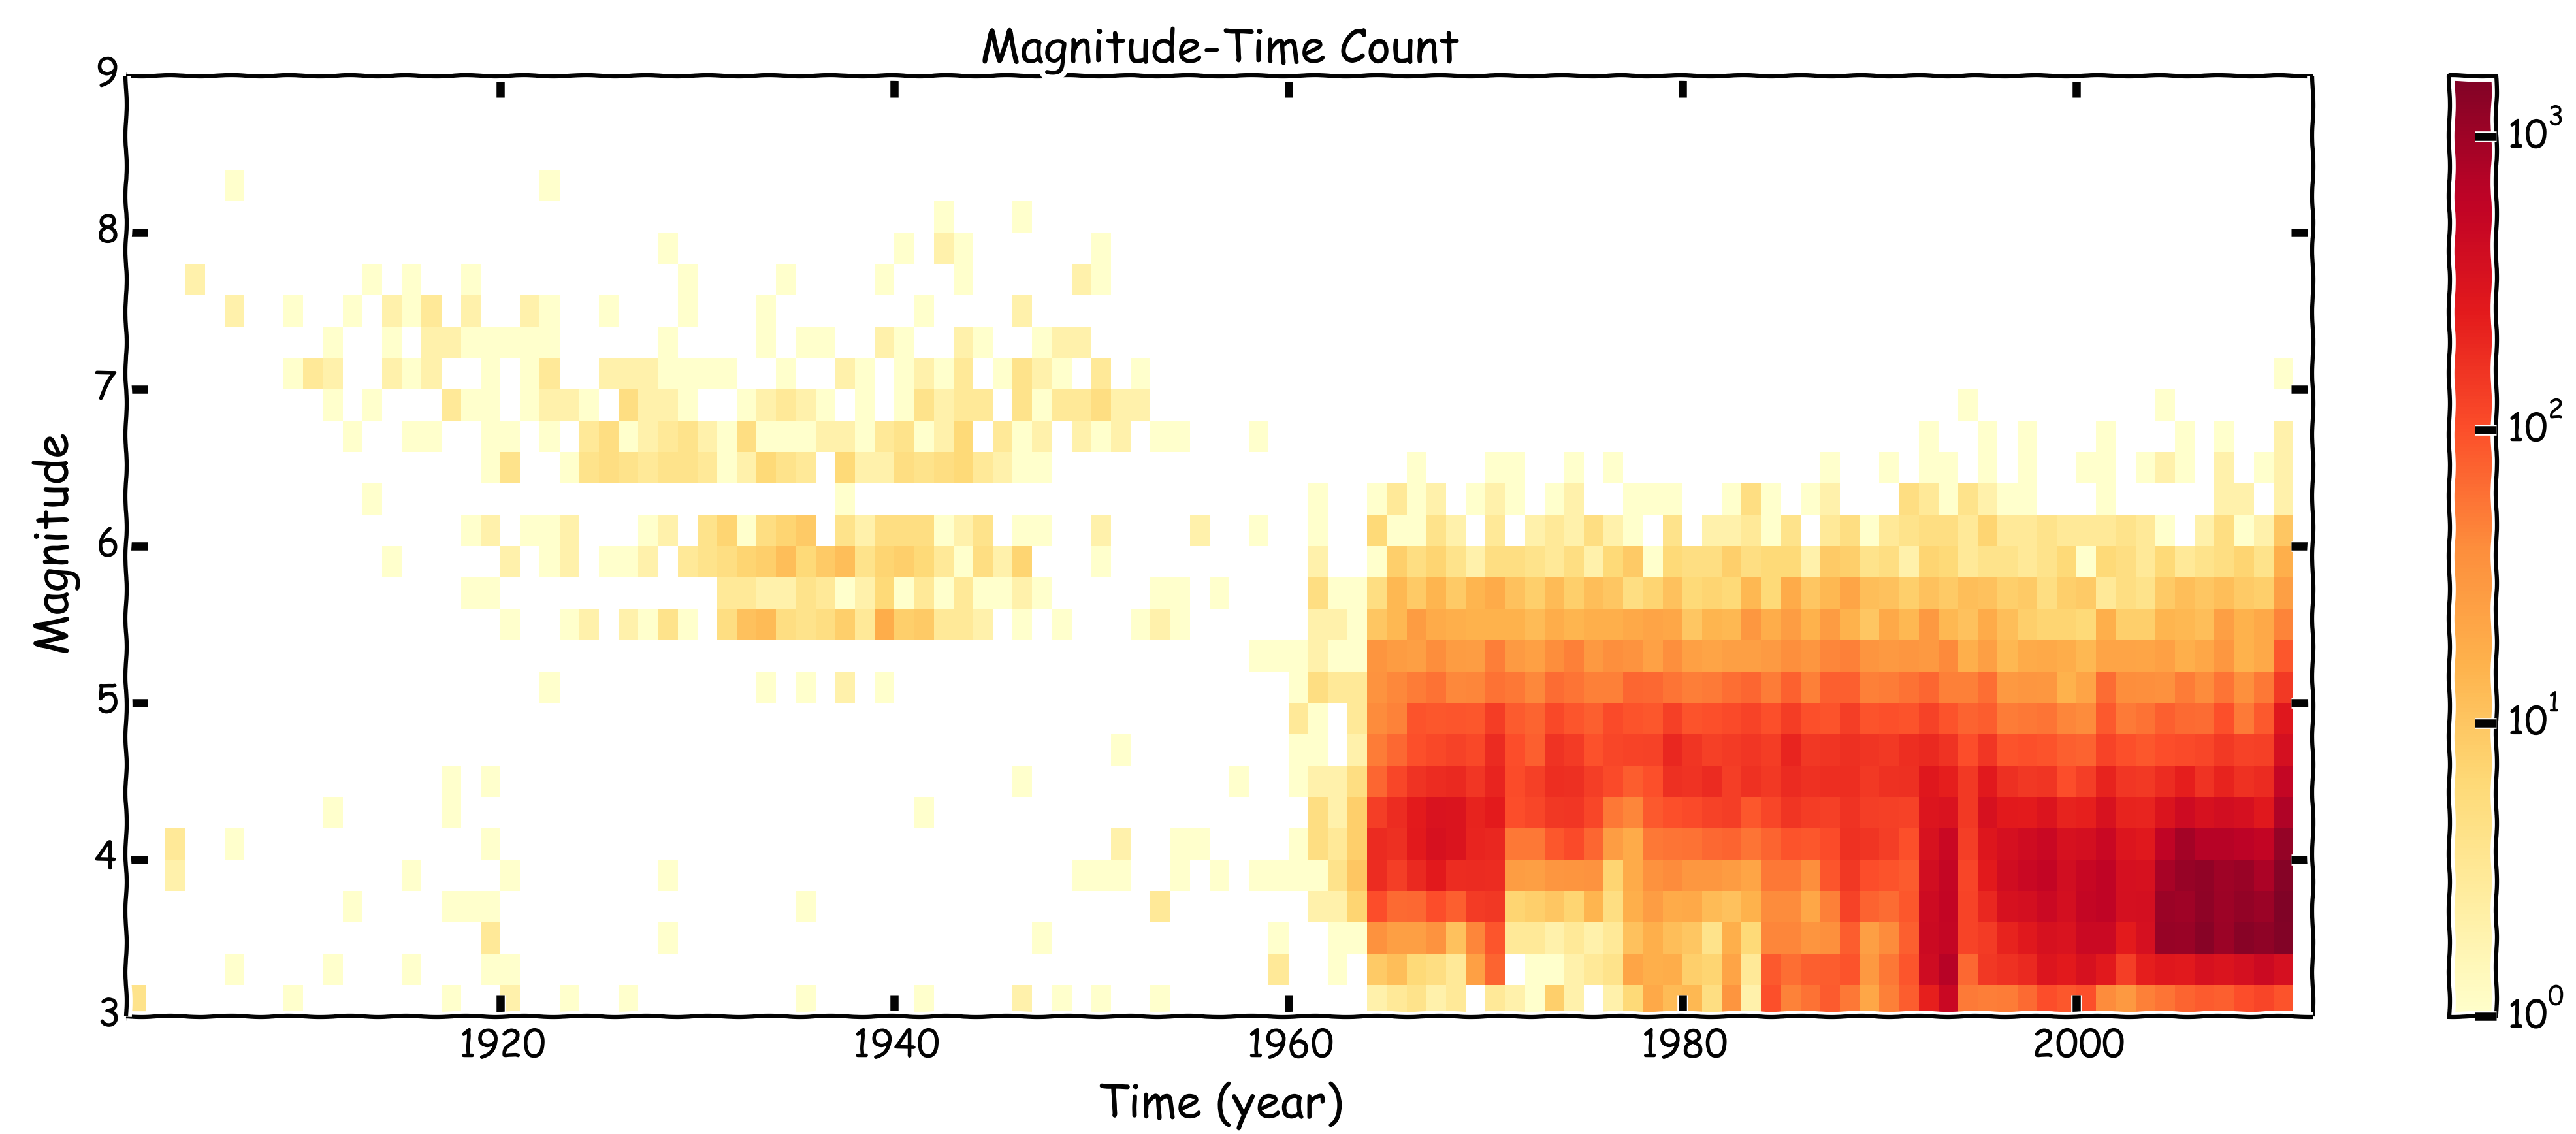
\includegraphics[width=0.95\textwidth]{time_mag_count_sa}
	\caption{Catálogo \gls{iscgem} 1900-2012}
	\label{fig:tmf_sa}
\end{figure}
\end{frame}


%-----------------------------------------------------------------------------
\begin{frame}{Distribuição Temporal de Magnitudes: \gls*{bsb2013}}
\begin{figure}[H]
	\centering
	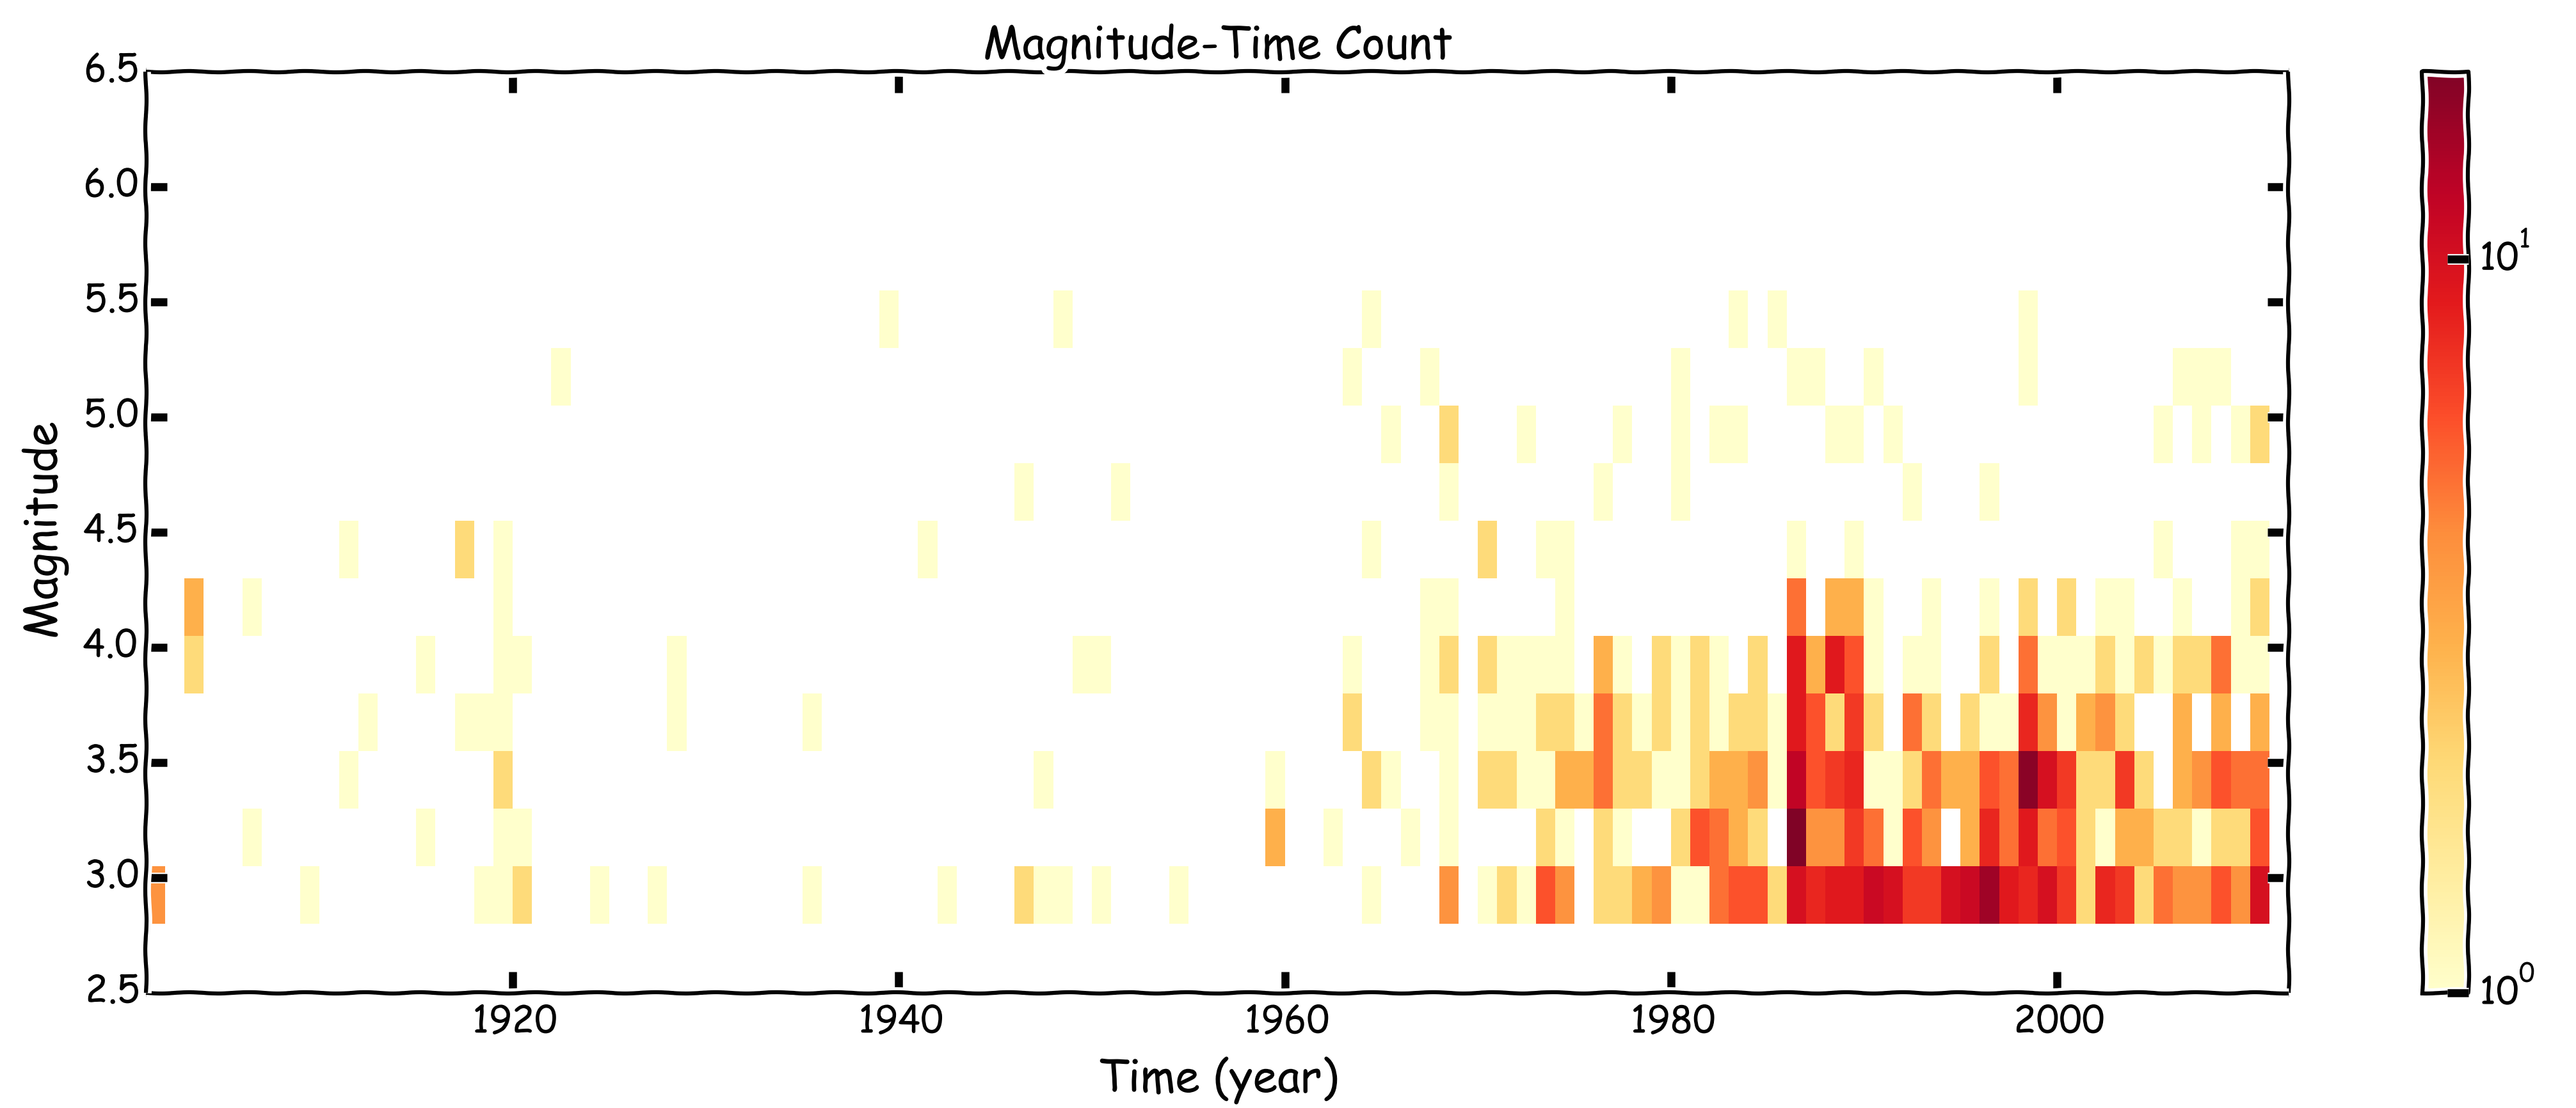
\includegraphics[width=0.95\textwidth]{time_mag_count_br}
	\caption{Catálogo \gls{bsb2013} 1900-2012}
	\label{fig:tmf_br_1960}
\end{figure}%
\end{frame}




%-----------------------------------------------------------------------------
\begin{frame}{Distribuição de Profundidades}
\begin{figure}[H]
	\centering
	\begin{subfigure}[t]{0.45\textwidth}
		  	\centering
			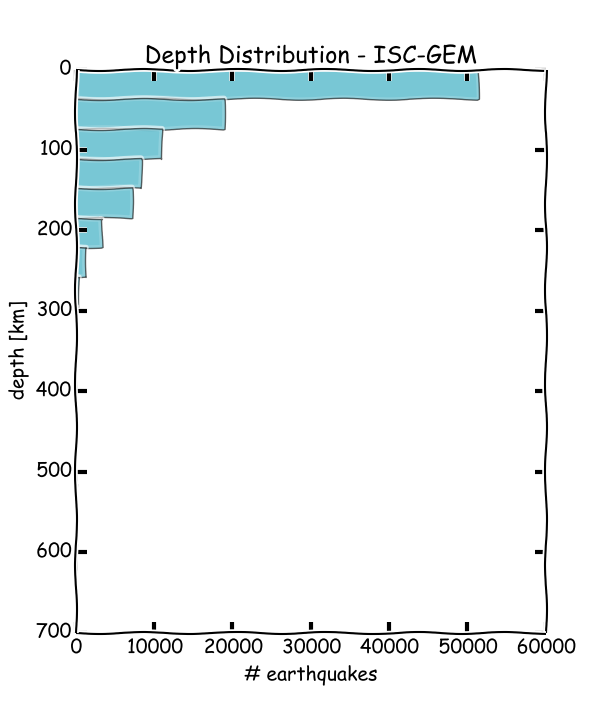
\includegraphics[width=1.00\textwidth]{dep_sa_hist}
			\subcaption{Distribuição da profundidade dos tremores, \gls{iscgem}}
			\label{fig:sa_dep_hist}
	\end{subfigure}%
	\quad %~ %add desired spacing between images, e. g. ~, \quad, \qquad, \hfill etc.
	\begin{subfigure}[t]{0.4\textwidth}
		  	\centering
			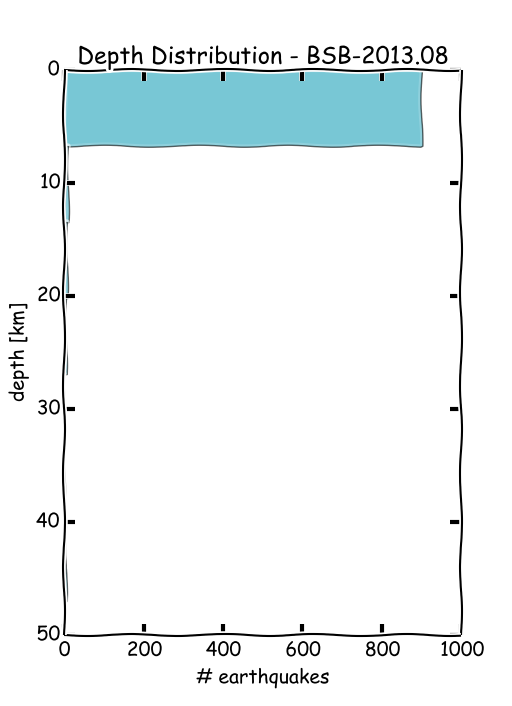
\includegraphics[width=1.00\textwidth]{dep_br_hist}
			\subcaption{Distribuição da profundidade dos tremores, \gls{bsb2013}}
			\label{fig:br_dep_hist}
        \end{subfigure}%
%  \caption{Profundidades.}
  \label{fig:qc_histograms} 
\end{figure}
\end{frame}




%-----------------------------------------------------------------------------
\begin{frame}{Número de sismos por dias da semana}
\begin{figure}[H]
	\centering
	\begin{subfigure}[t]{0.48\textwidth}
		  	\centering
			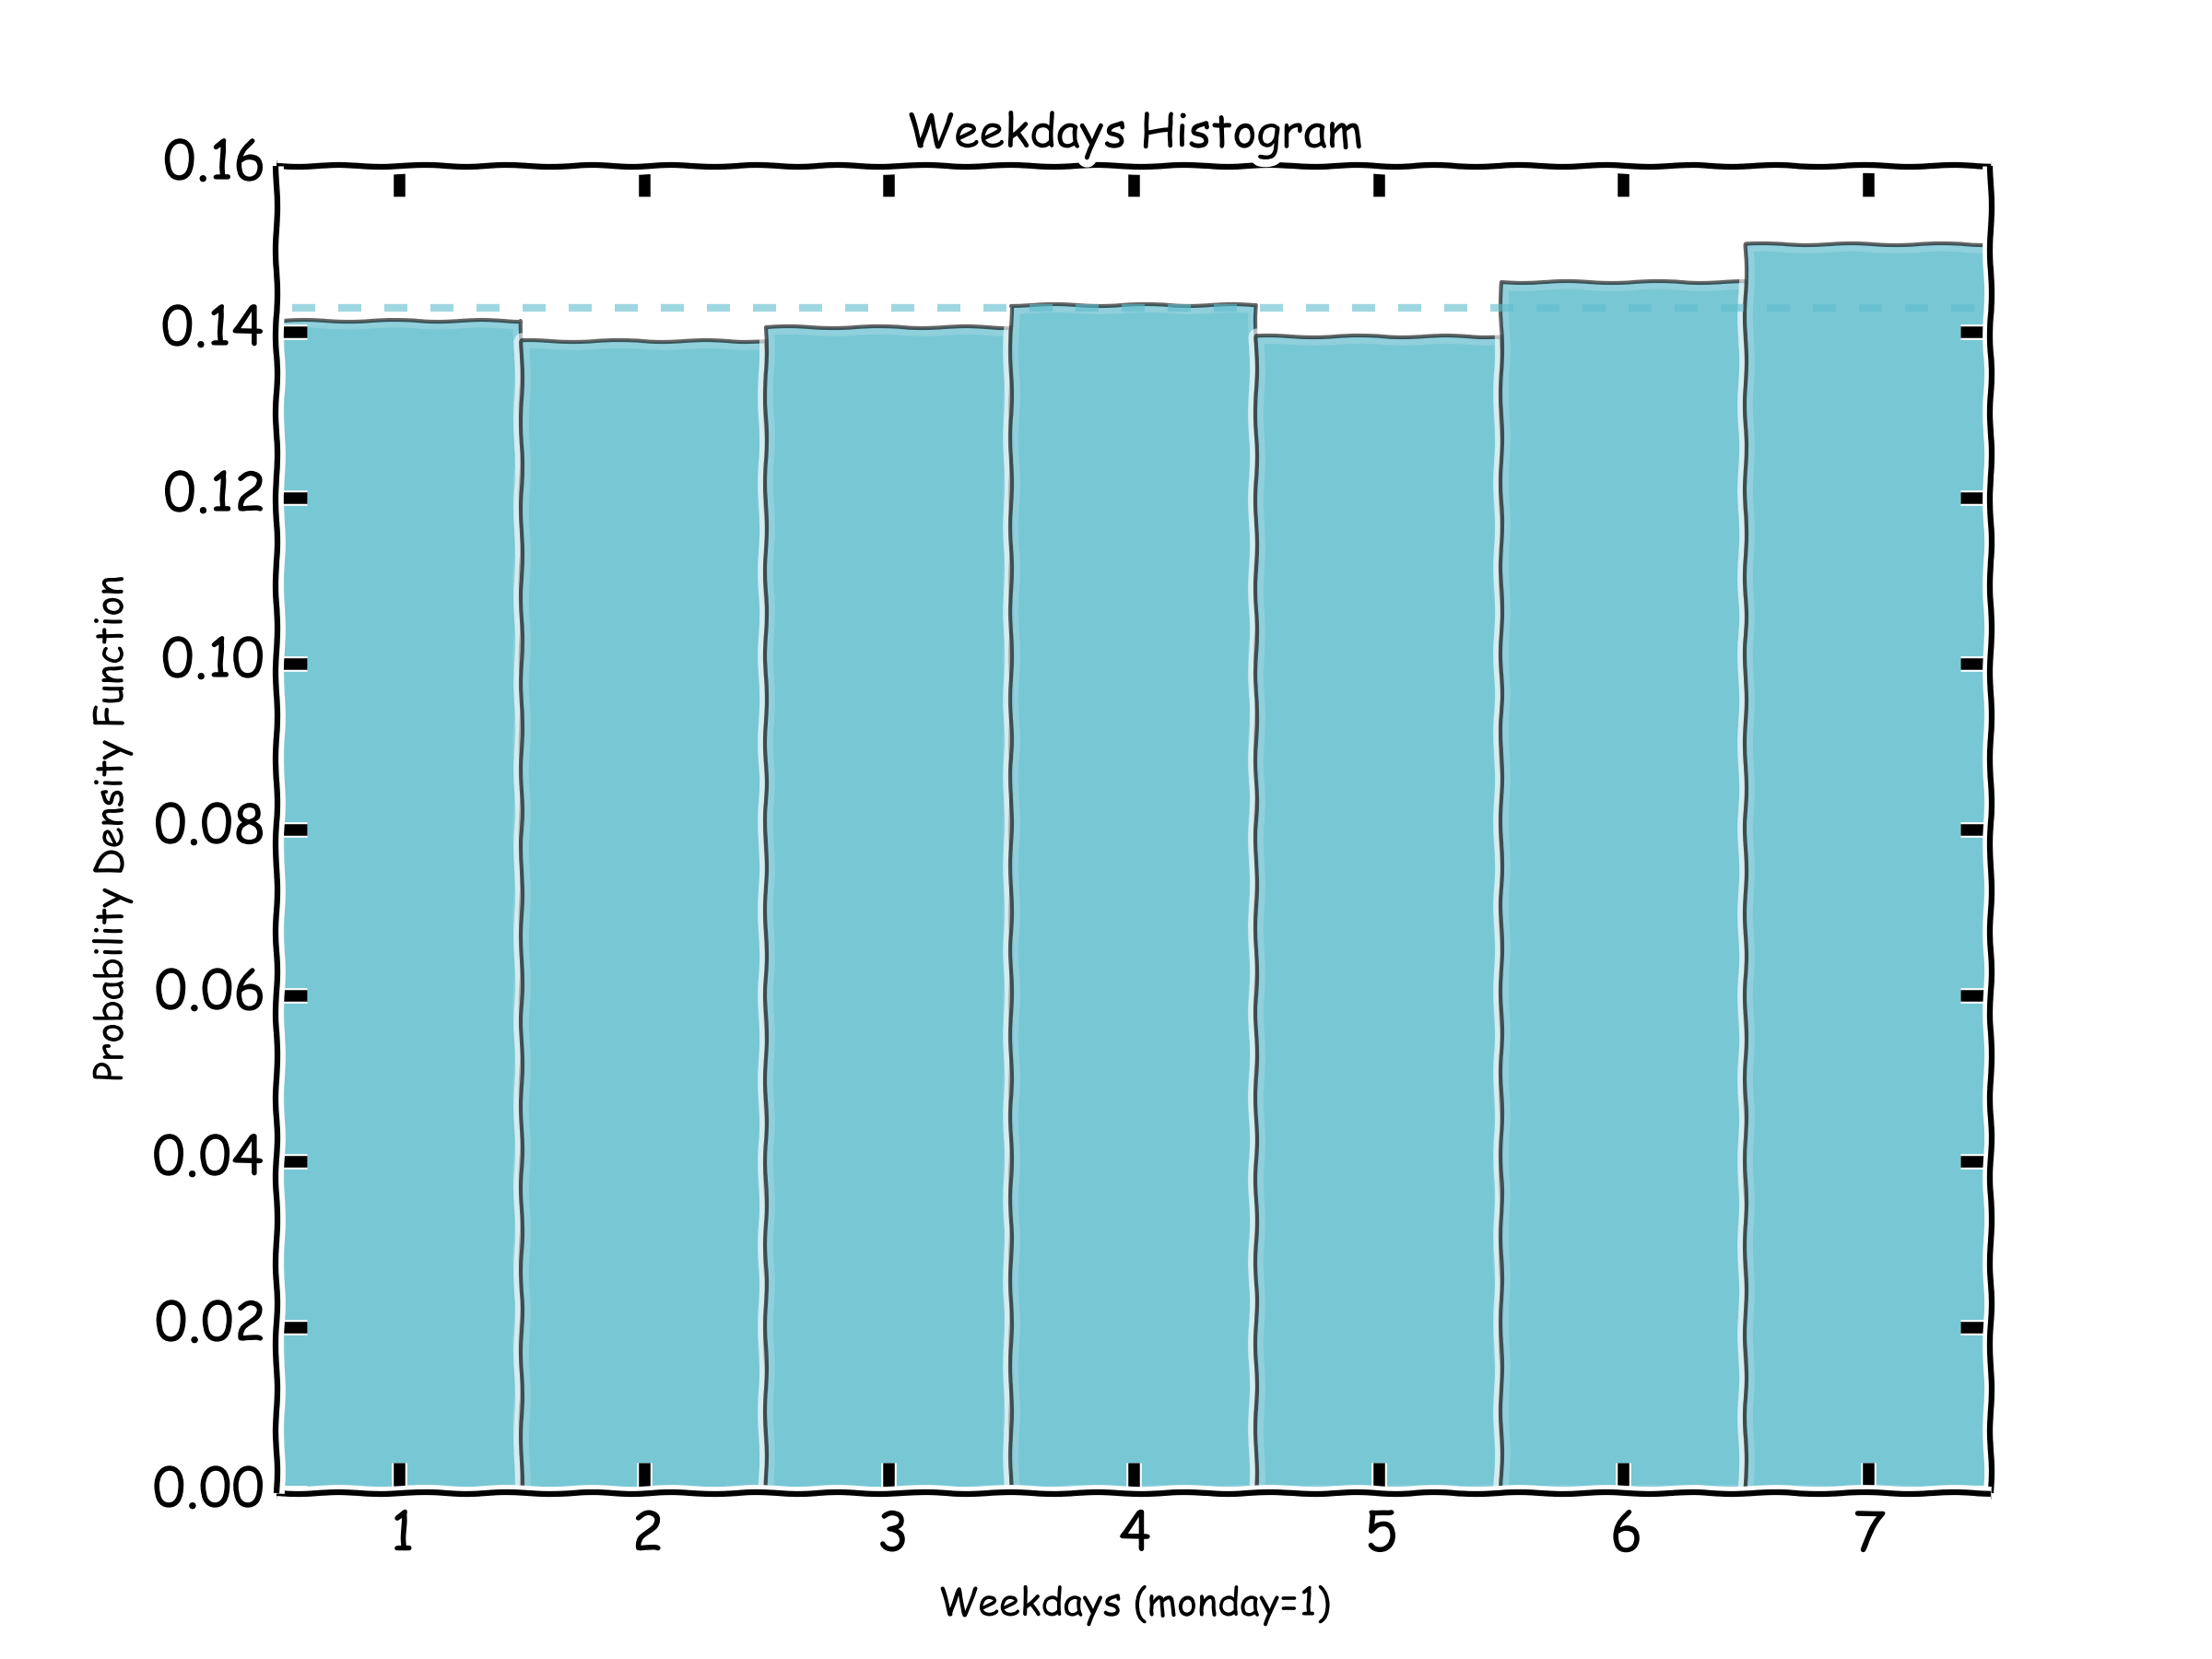
\includegraphics[width=1.0\textwidth]{hmtk_sa3_weekday}
			\subcaption{Distribuição dos tremores nos dias da semana, \gls{iscgem}}
			\label{fig:sa_week_hist}
	\end{subfigure}%
	\quad %~ %add desired spacing between images, e. g. ~, \quad, \qquad, \hfill etc.
	\begin{subfigure}[t]{0.48\textwidth}
		  	\centering
			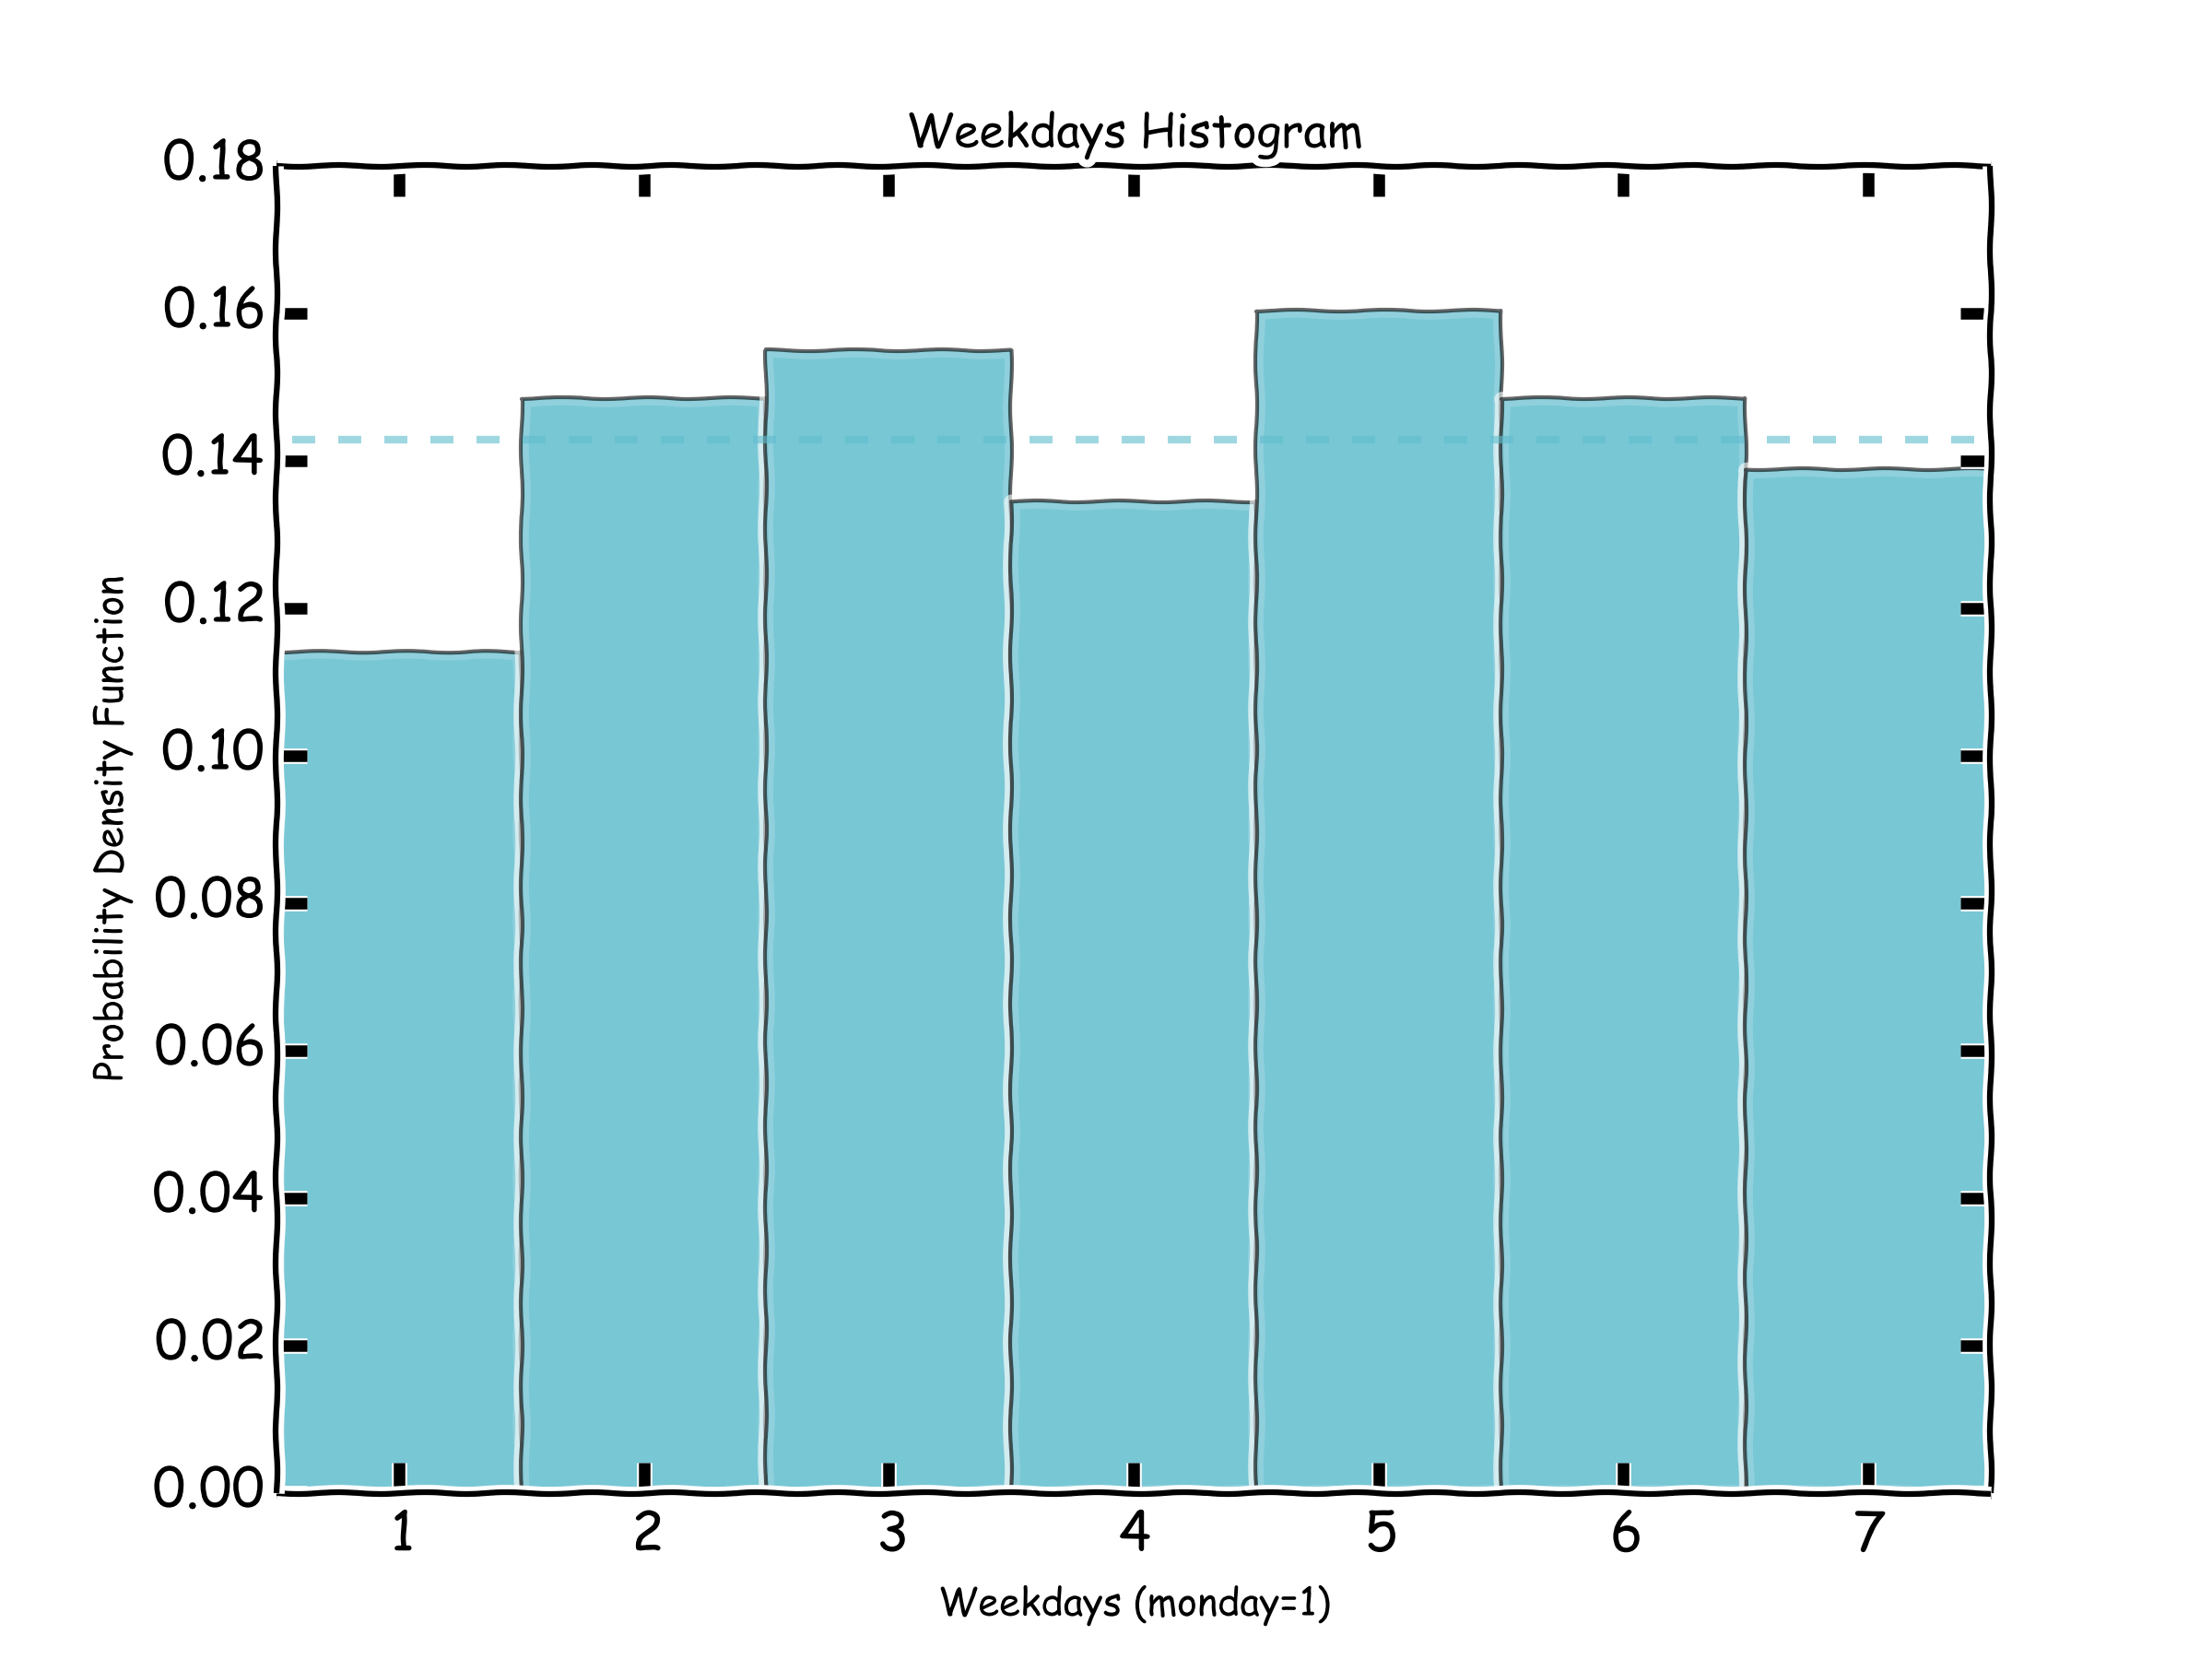
\includegraphics[width=1.0\textwidth]{hmtk_bsb2013_weekday}
			\subcaption{Distribuição dos tremores nos dias da semana, \gls{bsb2013}}
			\label{fig:br_week_hist}
    \end{subfigure}%
  %\caption{Checagem de qualidade.}
  \label{fig:qc_histograms} 
\end{figure}
\end{frame}



%-----------------------------------------------------------------------------
\begin{frame}{Distribuição da hora de ocorrência}
\begin{figure}[H]
	\centering
 	\begin{subfigure}[t]{0.45\textwidth}
		  	\centering
			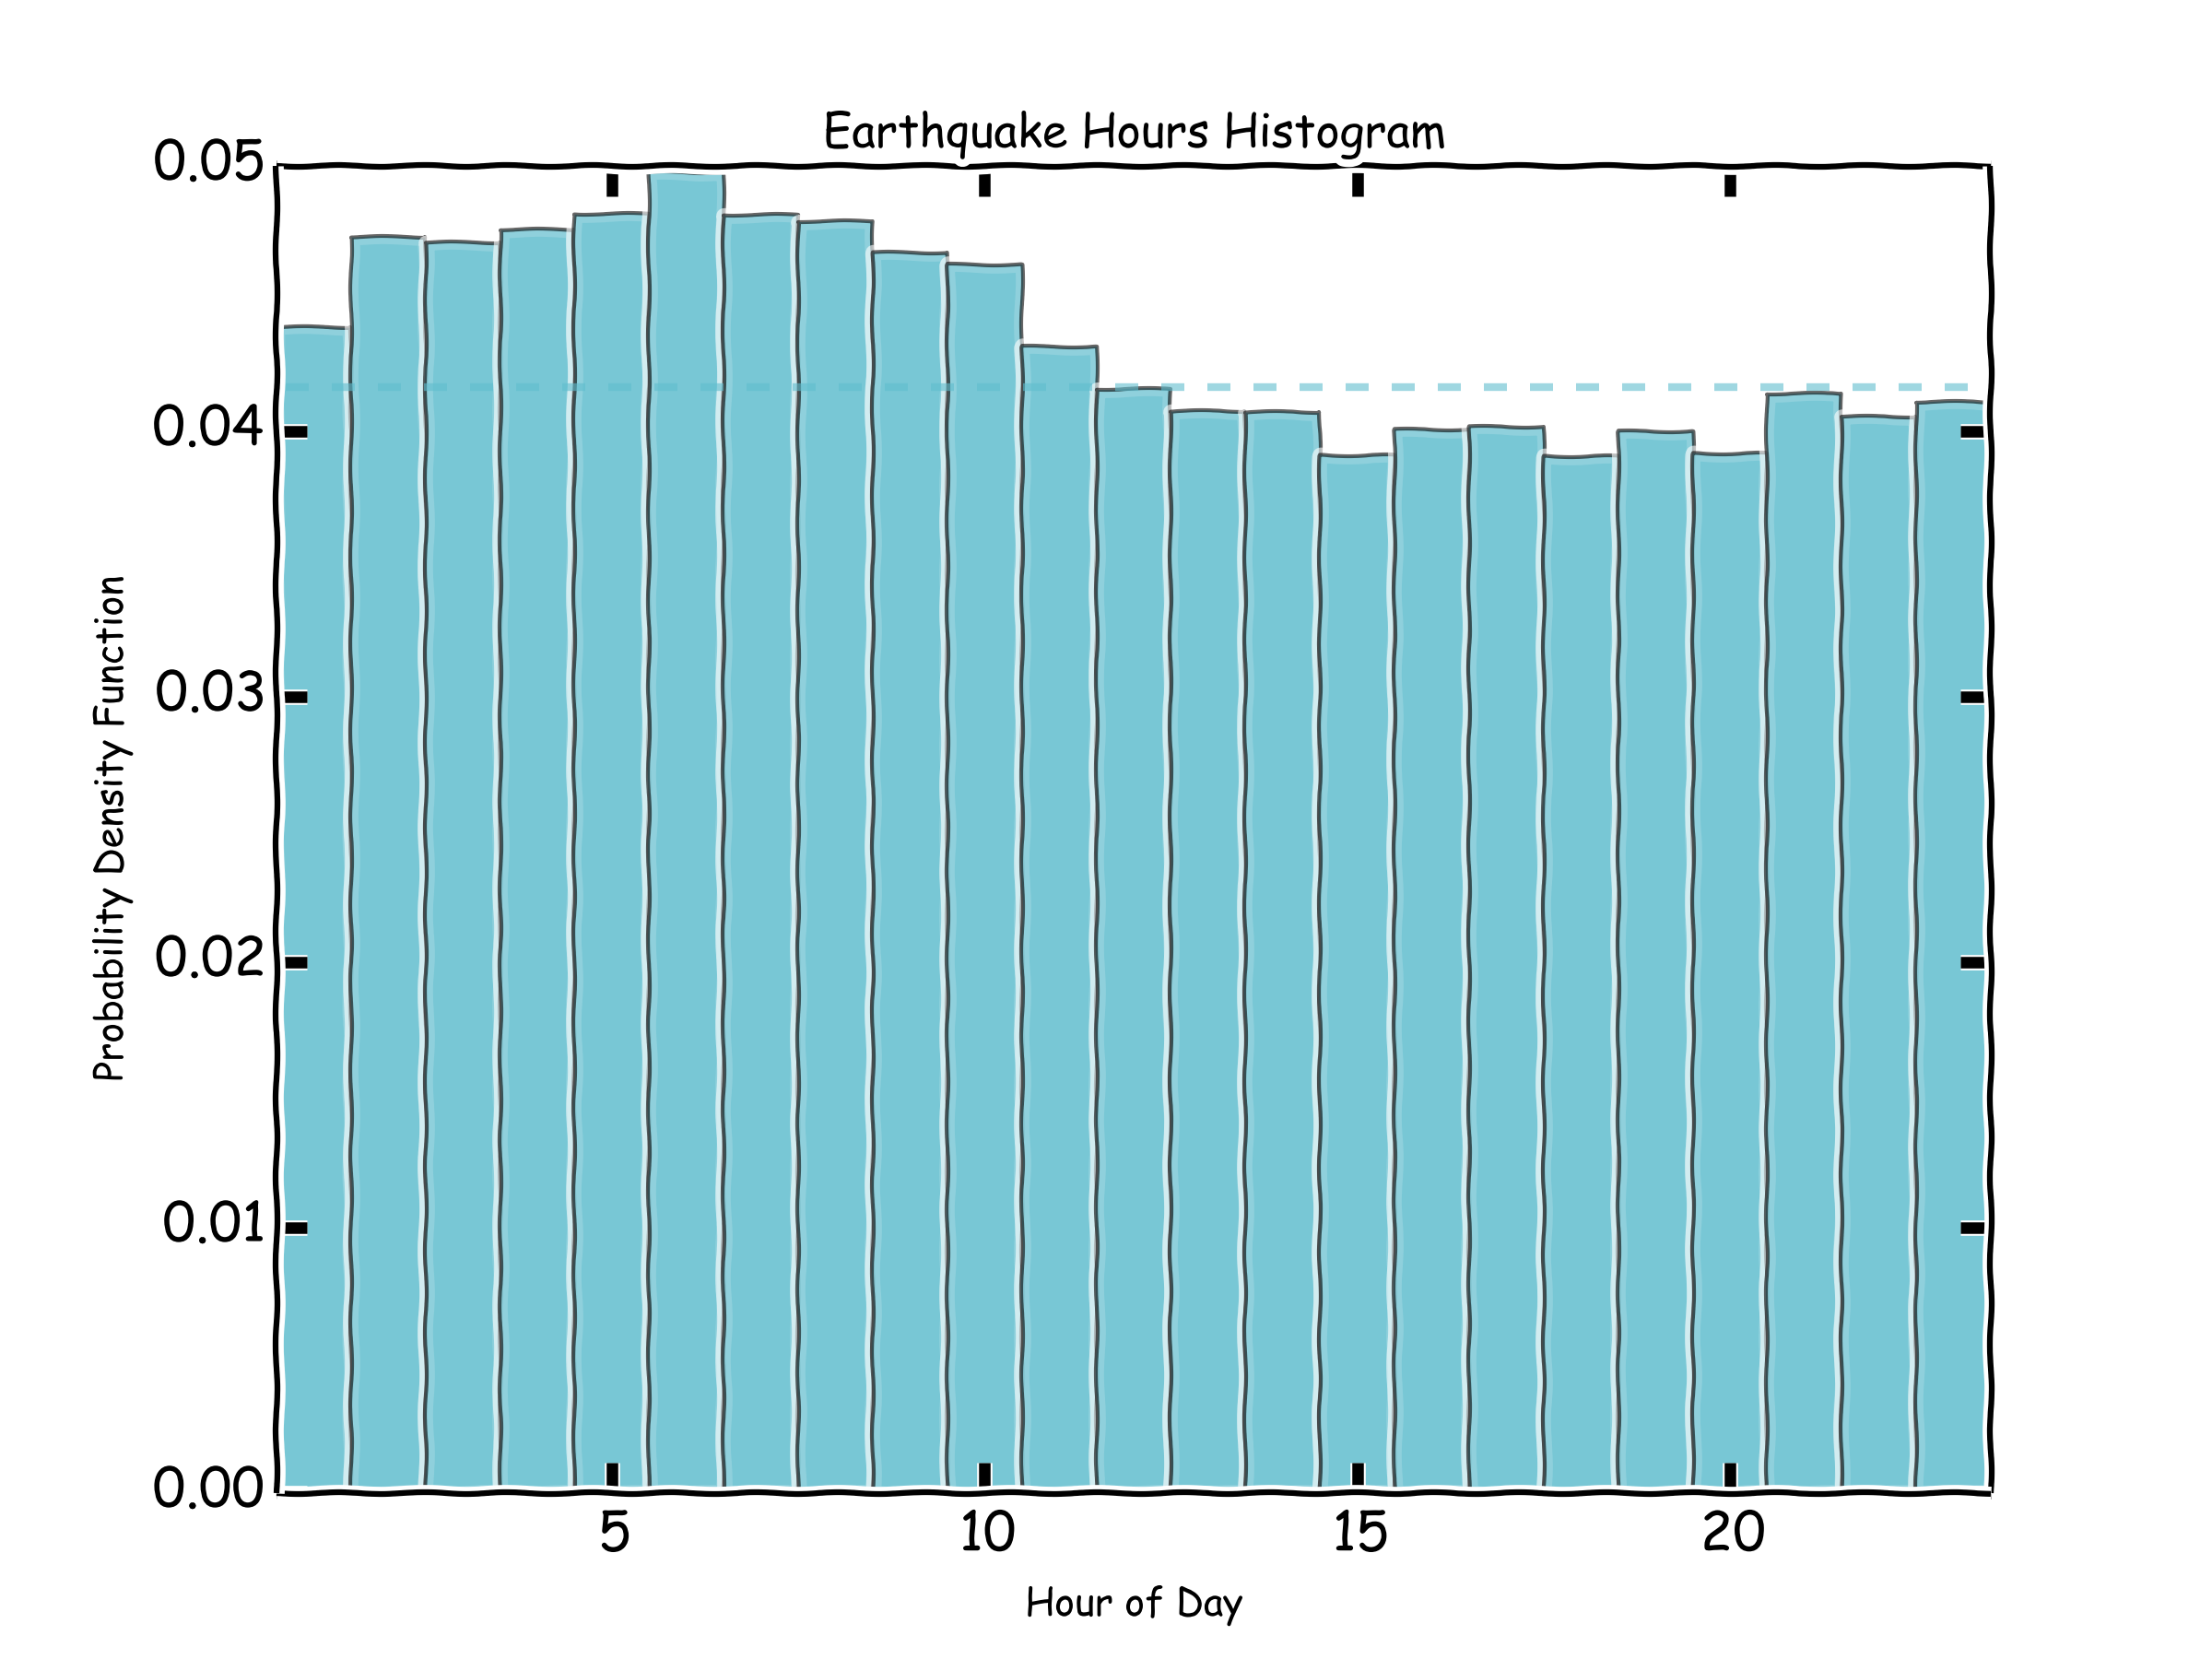
\includegraphics[width=1.00\textwidth]{hmtk_sa3_hour}
			\subcaption{Distribuição do horário de ocorrência dos tremores, \gls{iscgem}}
			\label{fig:sa_hour_hist}
	\end{subfigure}%
	\quad %~ %add desired spacing between images, e. g. ~, \quad, \qquad, \hfill etc.
	\begin{subfigure}[t]{0.45\textwidth}
		  	\centering
			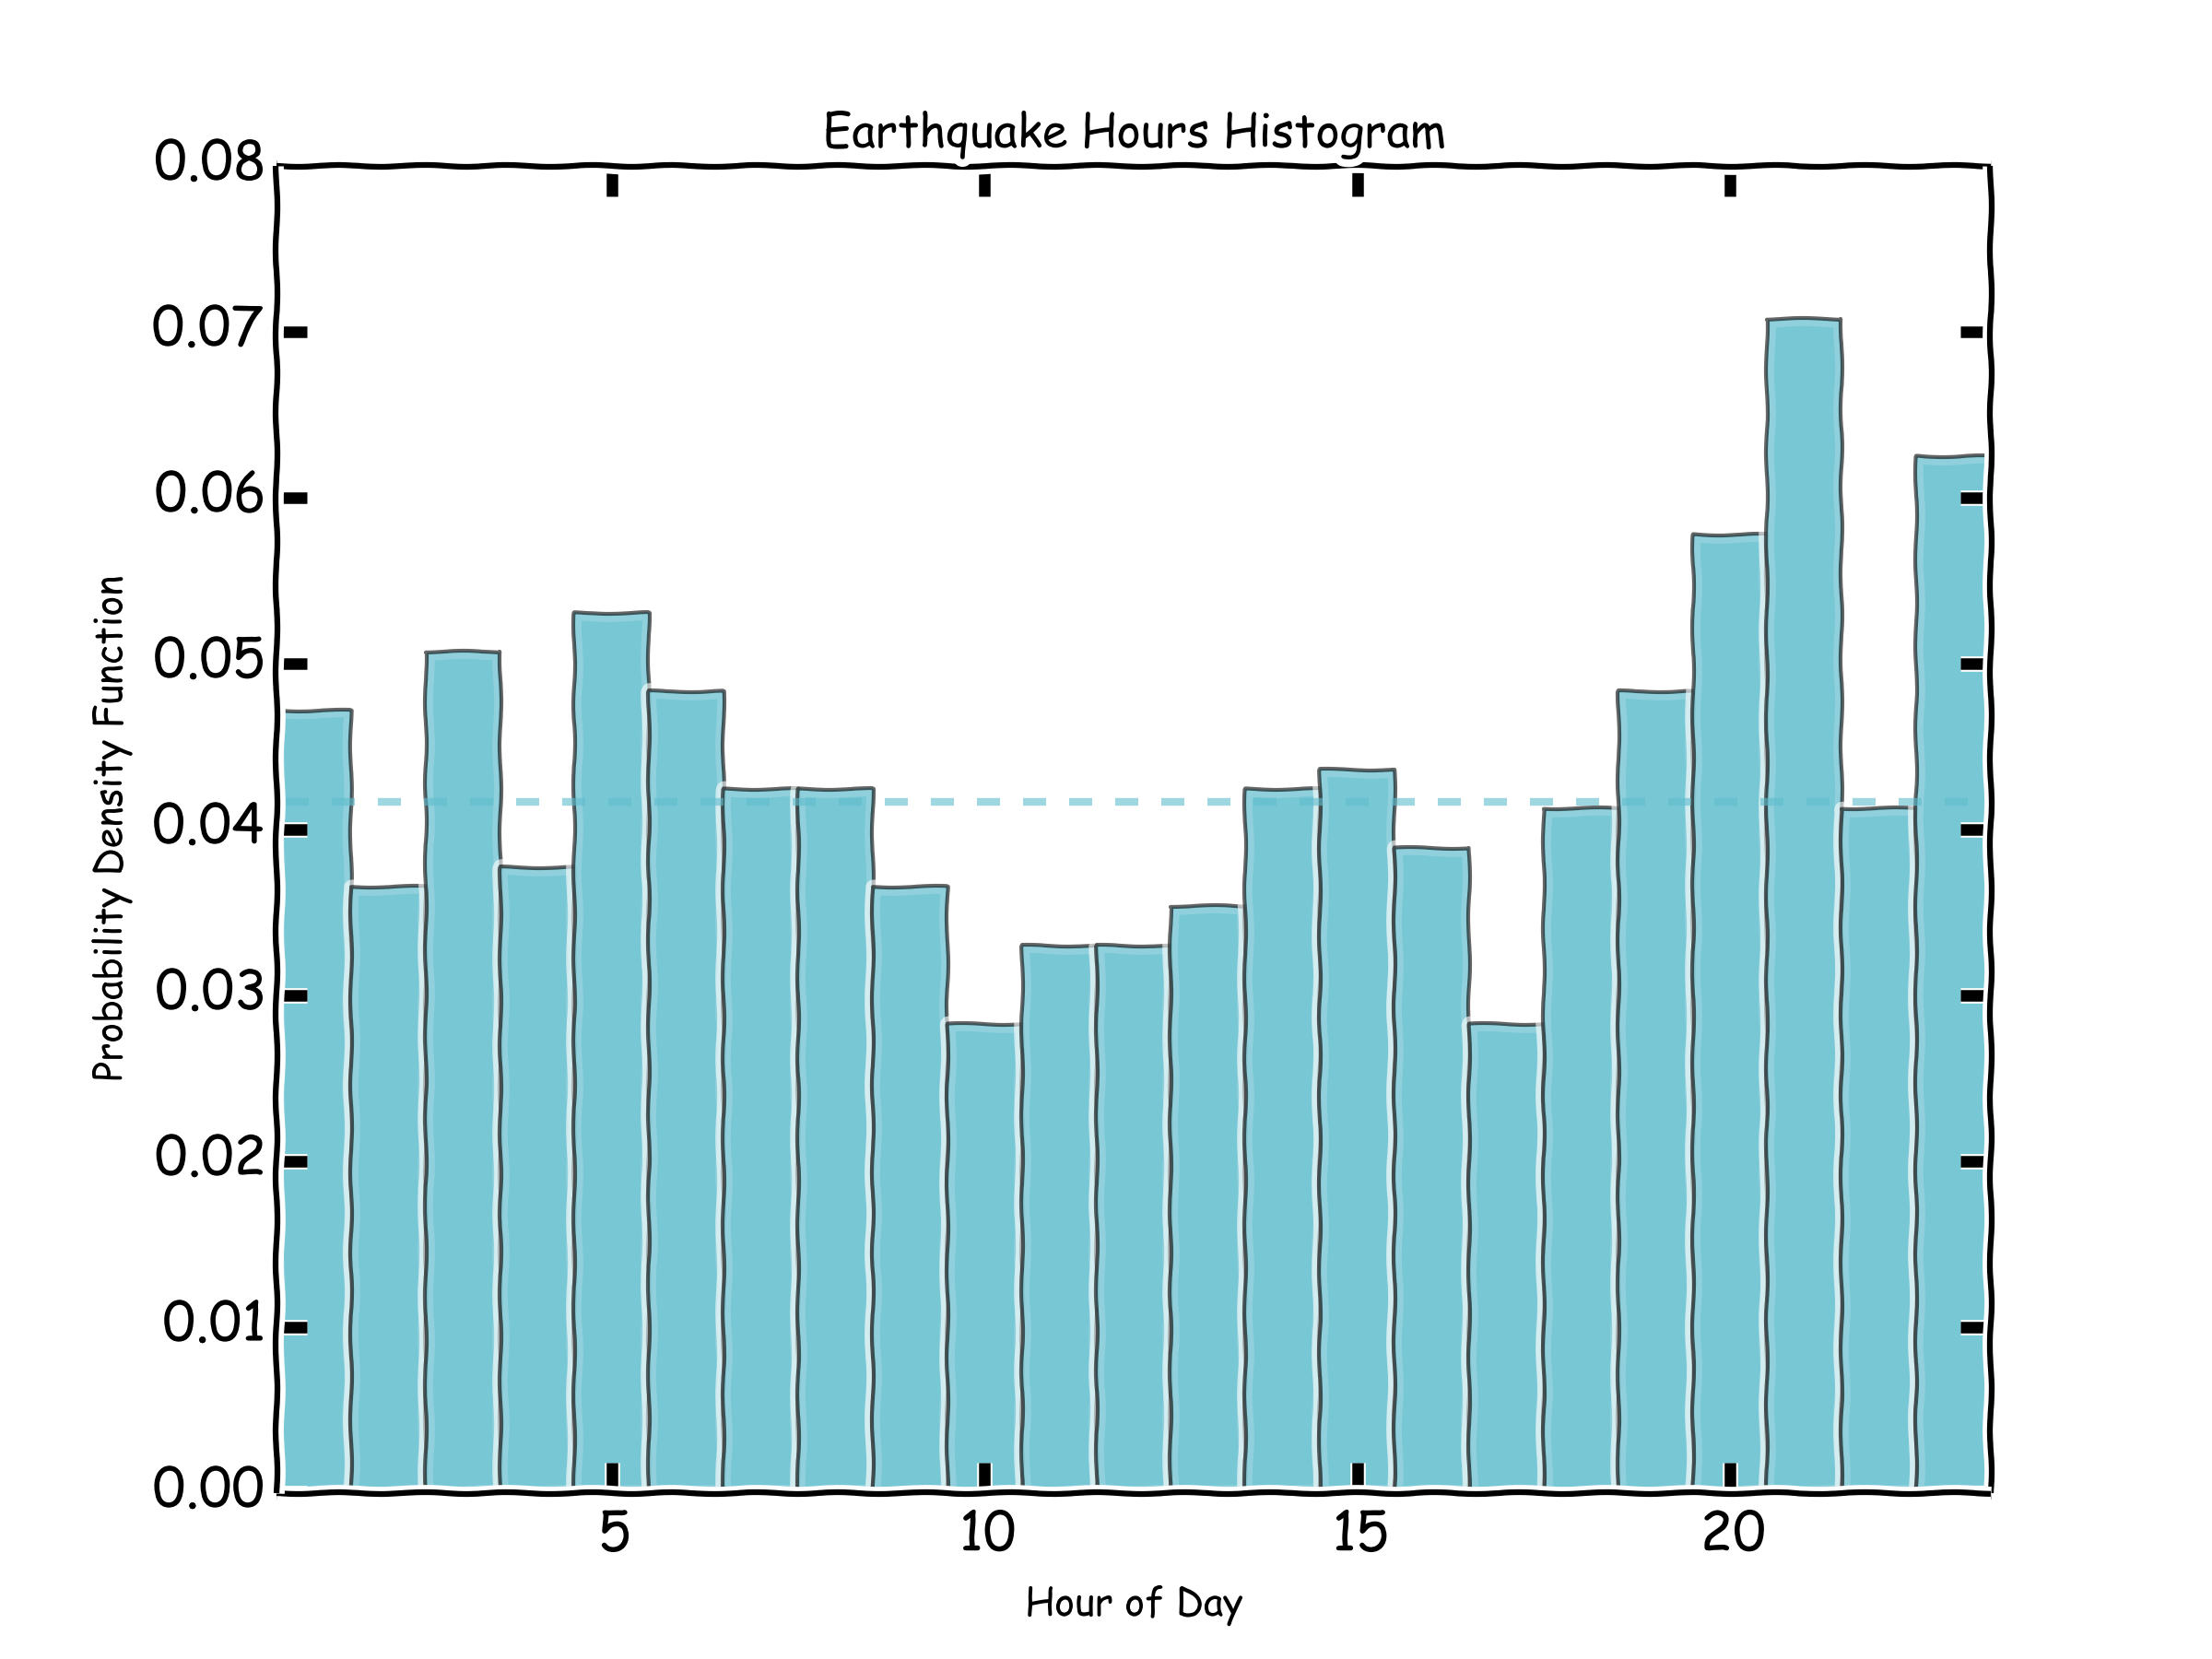
\includegraphics[width=1.00\textwidth]{hmtk_bsb2013_hour}
			\subcaption{Distribuição do horário de ocorrência dos tremores, \gls{bsb2013}}
			\label{fig:br_hour_hist}
    \end{subfigure}%
  %\caption{Checagem de qualidade.}
  \label{fig:qc_histograms} 
\end{figure}
\end{frame}




%=============================================================================
\subsection{Pré-processamento}
%=============================================================================

\subsubsection{Agrupamentos}

%-----------------------------------------------------------------------------
\begin{frame}{Remoção de Agrupamentos: \gls{bsb2013}}
\begin{figure}[H]
	\centering
	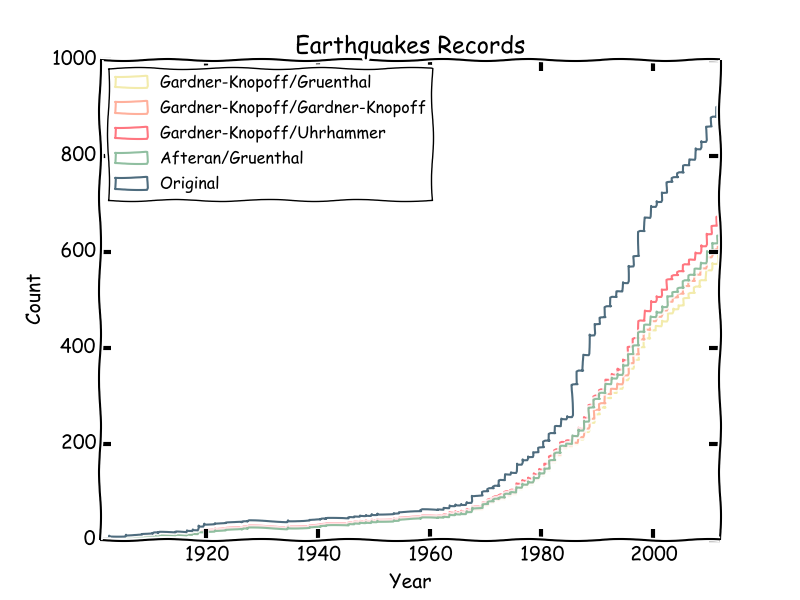
\includegraphics[height=0.90\textheight]{decluster_br}
	\caption{Número cumulativo de tremores registrados por ano para o \gls{bsb2013}
	original e para diferentes métodos/janelas de remoção de agrupamentos.}
	\label{fig:br_eq_record}
\end{figure}
\end{frame}


%-----------------------------------------------------------------------------
\begin{frame}{Remoção de Agrupamentos: \gls{iscgem}}
\begin{figure}[H]
	\centering
	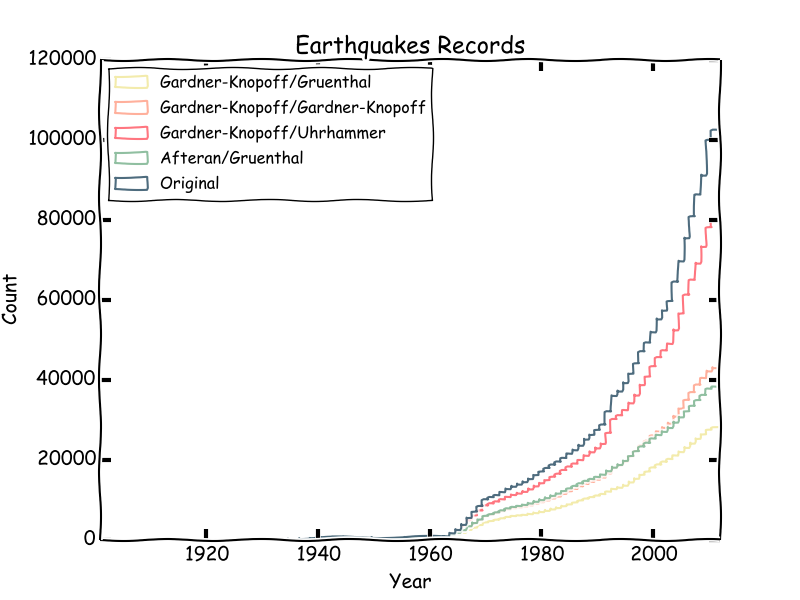
\includegraphics[height=0.90\textheight]{decluster_sa}
	\caption{Número cumulativo de tremores registrados por ano para o \gls{iscgem}
	original e para diferentes métodos/janelas de remoção de agrupamentos.}
	\label{fig:sa_eq_record}
	\end{figure}%
\end{frame}



%-----------------------------------------------------------------------------
\begin{frame}{Agrupamentos}
\begin{figure}[H]
	\centering
	\begin{subfigure}[t]{0.46\textwidth}
		  	\centering
			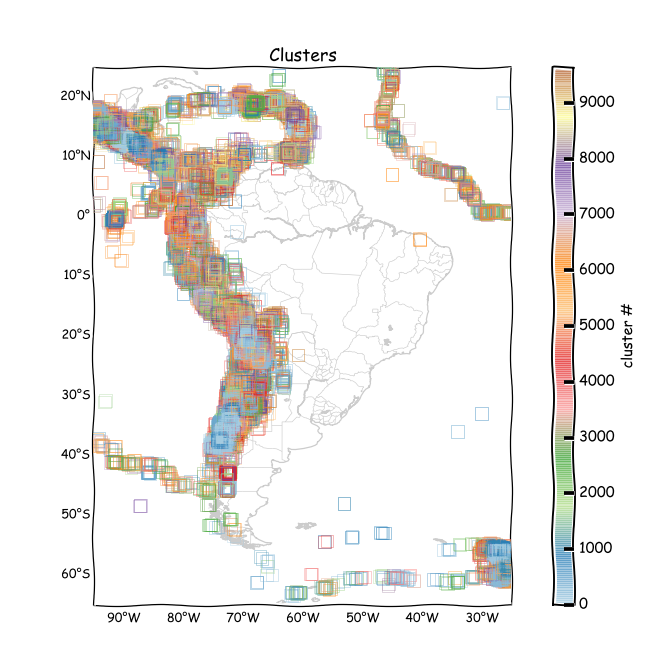
\includegraphics[width=1.00\textwidth]{hmtk_sa3_pp_decluster}
			\subcaption{Número de tremores registrados por ano, \gls{iscgem}}
			\label{fig:sa_decluster}
	\end{subfigure}%
	\quad %~ %add desired spacing between images, e. g. ~, \quad, \qquad, \hfill etc.
	\begin{subfigure}[t]{0.50\textwidth}
		  	\centering
			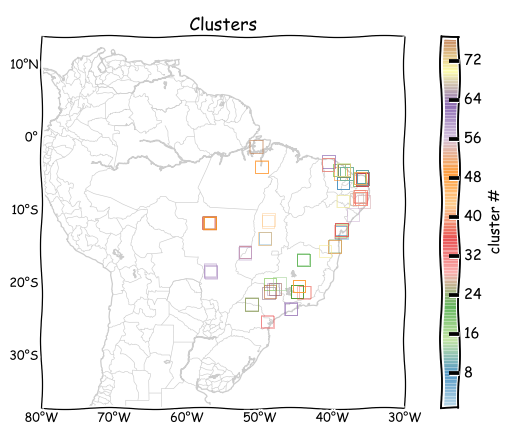
\includegraphics[width=1.00\textwidth]{hmtk_bsb2013_pp_decluster}
			\subcaption{Número de tremores registrados por ano, \gls{bsb2013}}
			\label{fig:br_decluster}
    \end{subfigure}%
	%\caption{Número de tremores registrados por ano após 1900}
	\label{fig:eq_decluster}
\end{figure}
\end{frame}


\subsubsection{Magnitude de Completude}



%-----------------------------------------------------------------------------
\begin{frame}{Método de Stepp: \gls{iscgem}}
\begin{figure}[H]
	\centering
	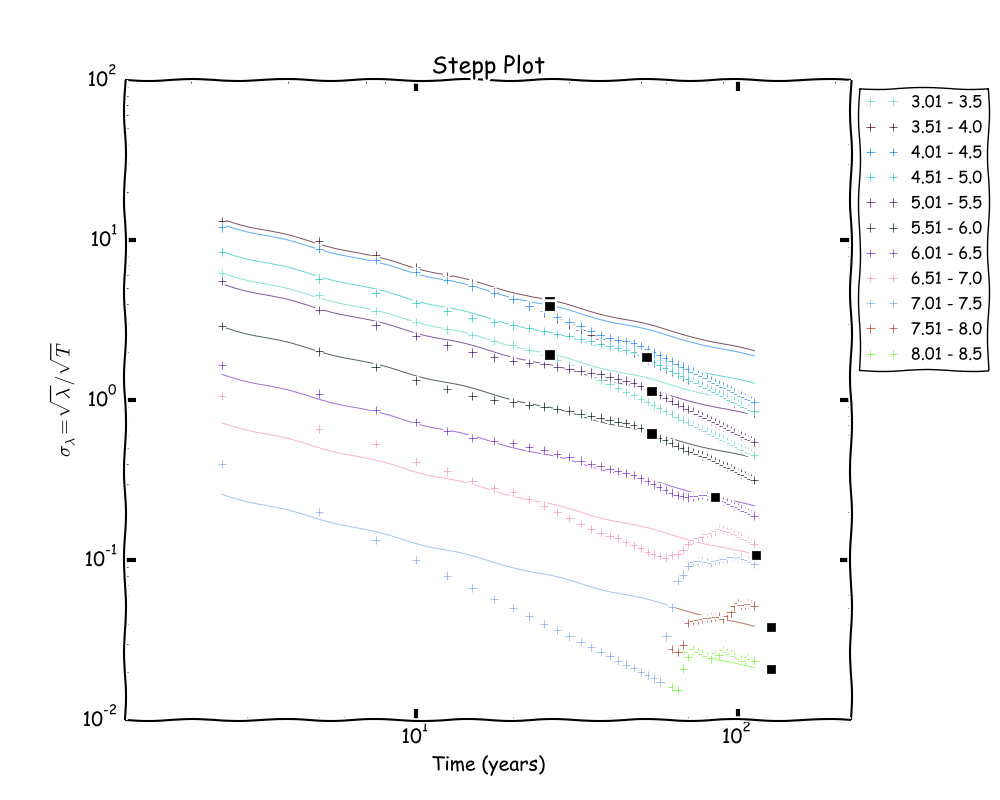
\includegraphics[height=0.90\textheight]{stepp_sa}
	\caption{Diagrama de Stepp para o \gls{iscgem} (\emph{declustered})}
	\label{fig:sa_stepp}
\end{figure}
\end{frame}


%-----------------------------------------------------------------------------
\begin{frame}{Método de Stepp: \gls{bsb2013}}
\begin{figure}[H]
	\centering
	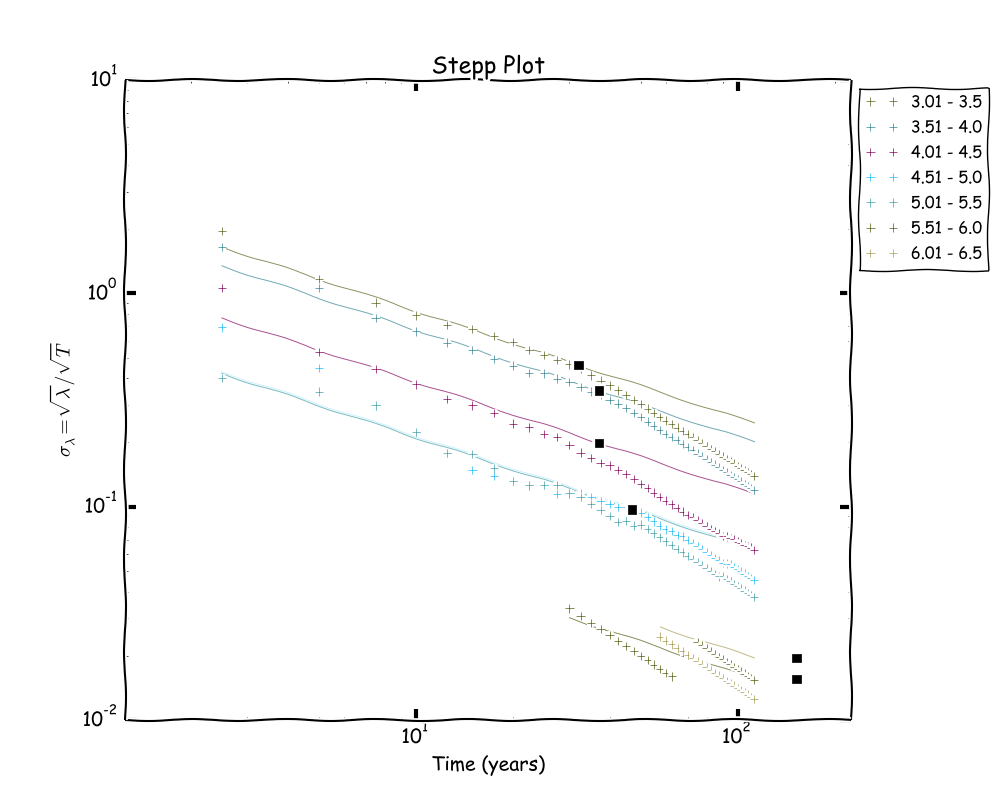
\includegraphics[height=0.90\textheight]{stepp_br}
	\caption{Diagrama de Stepp para o \gls{bsb2013} (\emph{declustered})}
	\label{fig:br_stepp}
\end{figure}
\end{frame}



%-----------------------------------------------------------------------------
\begin{frame}[c]{Magnitudes de Completude}
	\begin{table}[h]
	  	\centering
	  	\footnotesize
		\begin{tabular}{l|*{11}{c}}
		$M_c$ & 3.0  & 3.5  & 4.0  & 4.5  & 5.0  & 5.5  & 6.0  & 6.5  & 7.0  & 7.5  & 8 \\  \hline
		Ano   & 1986 & 1986 & 1986 & 1960 & 1958 & 1958 & 1927 & 1898 & 1885 & 1885 & 1885   \\
		\end{tabular}
		\caption{Magnitude de completude, \gls{iscgem}}
		\label{tab:mc_sa}
	\end{table} \\
	\quad		\\
	\quad		\\
	\begin{table}[h]
	  	\centering
	  	\footnotesize
		\begin{tabular}{l|*{7}{c}}
		$M_c$ & 3.0  & 3.5  & 4.0  & 4.5  & 5.0  & 5.5  & 6.0  \\  \hline
		Ano   & 1980 & 1975 & 1975 & 1965 & 1965 & 1860 & 1860 \\
		\end{tabular}
		\caption{Magnitude de completude, \gls{bsb2013}}
		\label{tab:mc_br}
	\end{table}
\end{frame}



%=============================================================================
\section{Técnicas de Suavização}
%=============================================================================

%=============================================================================
\subsection{Frankel, 1995}
%=============================================================================

%-----------------------------------------------------------------------------
\begin{frame}{Frankel1995: Taxa de Sismicidade (\gls{bsb2013})}
\begin{figure}[H]
  \centering
  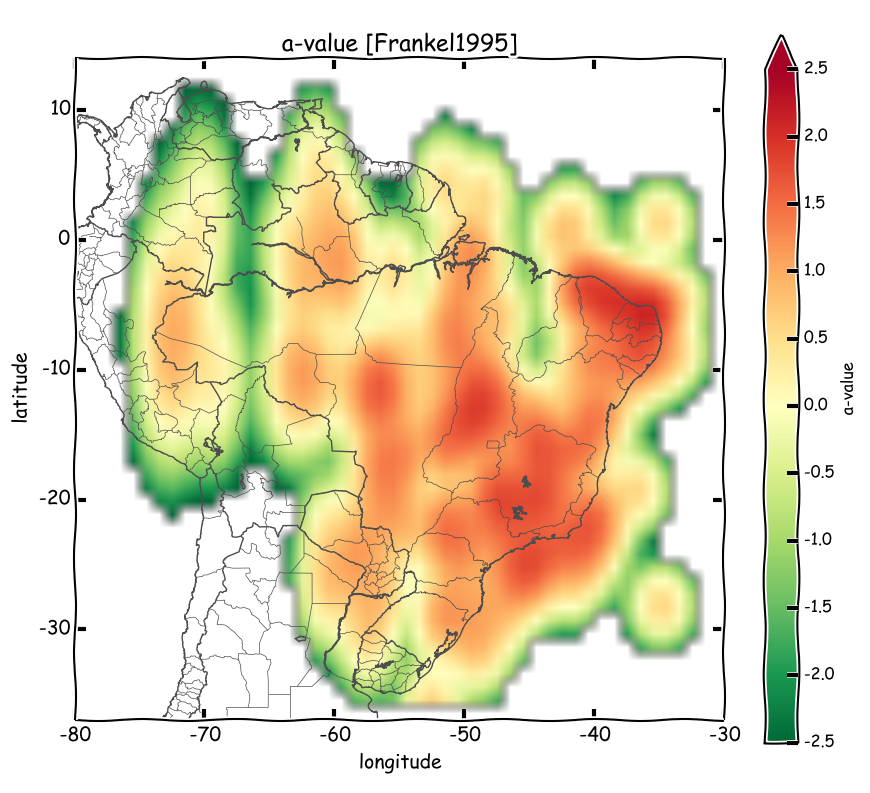
\includegraphics[height=.95\textheight]{a_frankel_br} 
  \caption{Mapa do valor-a, usando o catálogo \gls{bsb2013} calculado pelo método de Frankel, 1995 }
  \label{fig:a_fran_br} 
\end{figure}
\end{frame}



%-----------------------------------------------------------------------------
\begin{frame}{Frankel1995: Taxa de Sismicidade (\gls{iscgem})}
\begin{figure}[H]
  \centering
  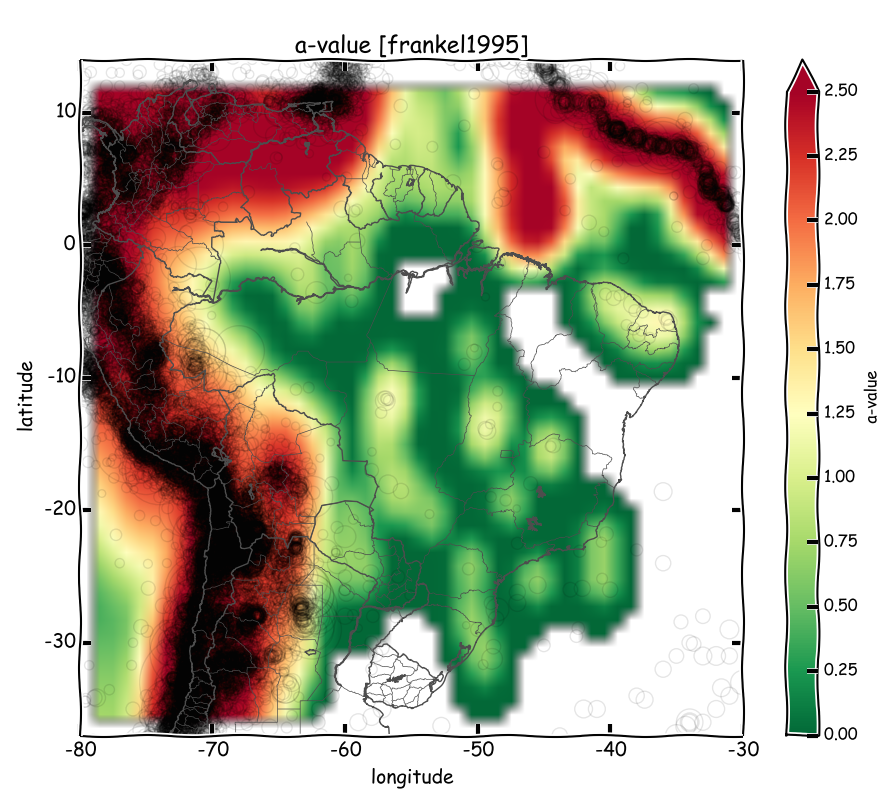
\includegraphics[height=.95\textheight]{a_frankel_sa} 
  \caption{Mapa do valor-a, catálogo \gls{iscgem} [Frankel, 1995] }
  \label{fig:a_fran_sa} 
\end{figure}
\end{frame}


%-----------------------------------------------------------------------------
\begin{frame}{Frankel1995: Ameaça}
\begin{figure}[H]
  \centering
  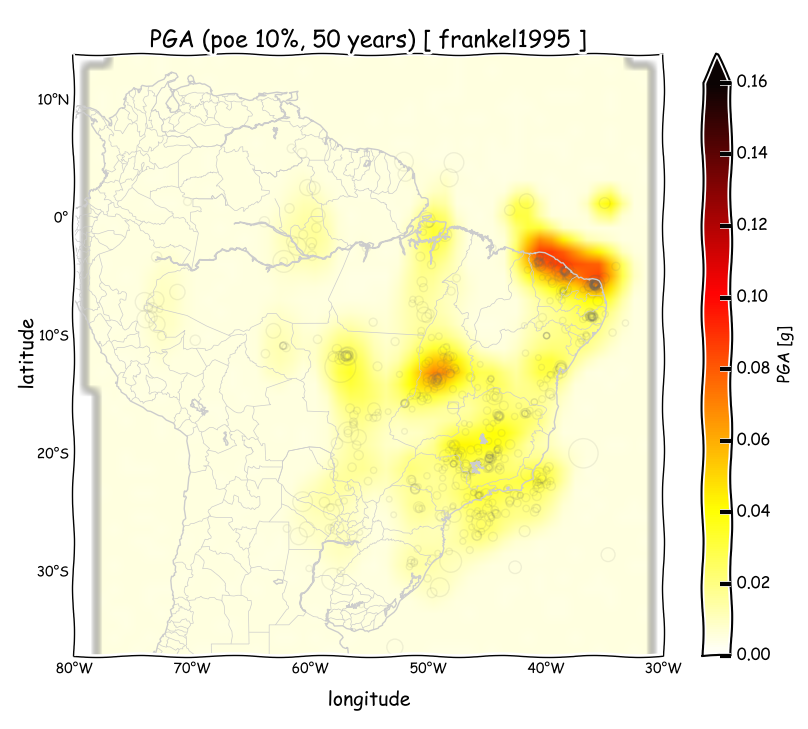
\includegraphics[height=.95\textheight]{pga_frankel} 
  \caption{Mapa de ameaça sísmica, PGA (poe 10\%, 50y) [Frankel, 1995] }
  \label{fig:pga_fran} 
\end{figure}
\end{frame}





%=============================================================================
\subsection{Woo, 1996}
%=============================================================================


%-----------------------------------------------------------------------------
\begin{frame}{Woo1996: Ajuste da largura de banda}
\begin{figure}[H]
  \centering
  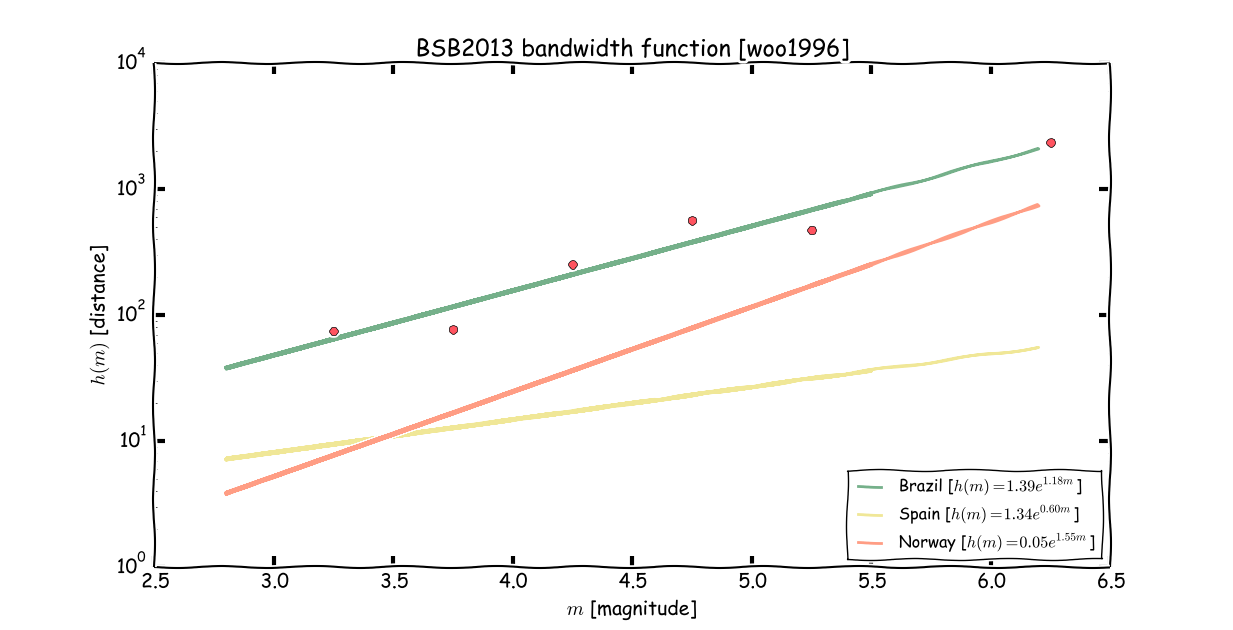
\includegraphics[width=.90\textwidth]{woo_bandwidth} 
  \caption{Ajuste da largura de banda para o método de Woo1996}
  \label{fig:woo_b} 
\end{figure}
\end{frame}


%-----------------------------------------------------------------------------
\begin{frame}{Woo1996: Taxa de Sismicidade (\gls{bsb2013})}

\begin{figure}[H]
  \centering
  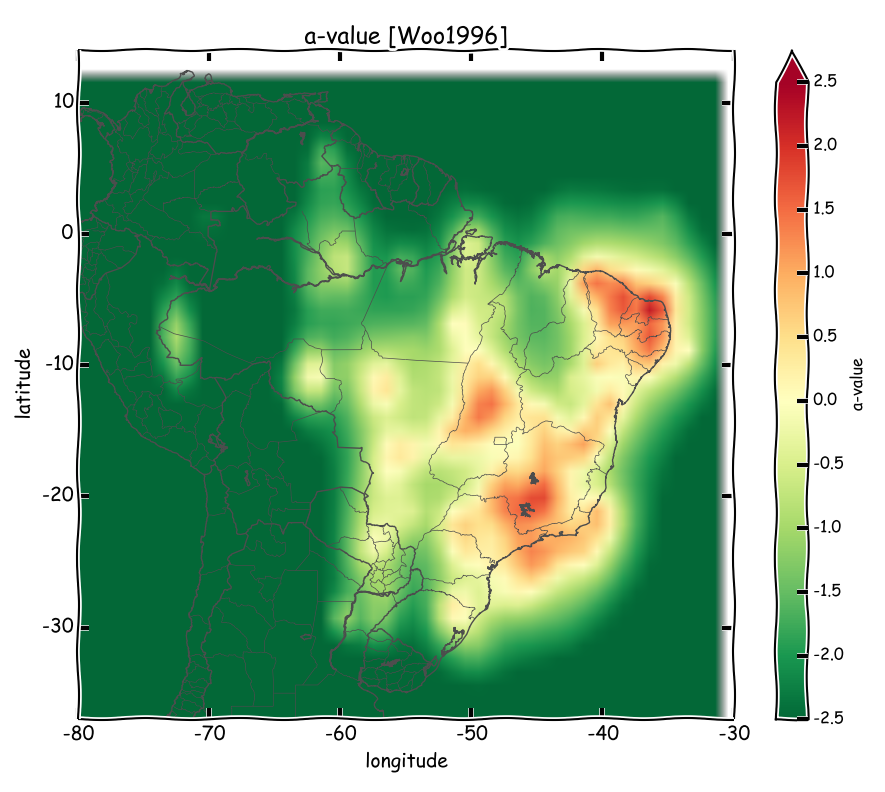
\includegraphics[height=.95\textheight]{a_woo} 
  \caption{Mapa do valor-a, usando o catálogo \gls{bsb2013} calculado pelo método de Woo, 1996 }
  \label{fig:a_woo} 
\end{figure}

\end{frame}



%-----------------------------------------------------------------------------
\begin{frame}{Woo1996: Ameaça (MFD discreta e incremental)}
\begin{figure}[H]
  \centering
  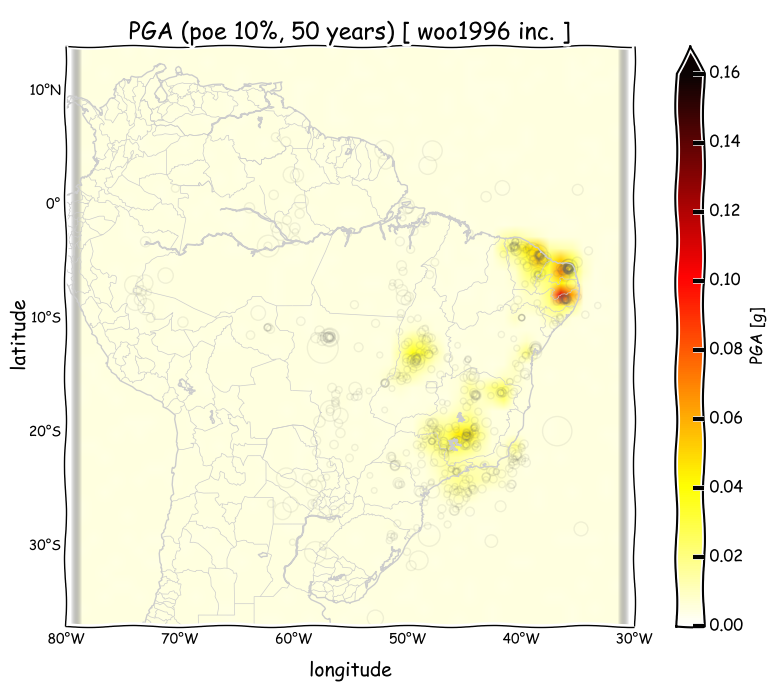
\includegraphics[height=.95\textheight]{pga_woo_inc} 
  \caption{Mapa de ameaça sísmica, PGA (poe 10\%, 50y).}
  \label{fig:pga_woo_inc} 
\end{figure}
\end{frame}



%-----------------------------------------------------------------------------
\begin{frame}{Woo1996: Ameaça (MFD truncada)}
\begin{figure}[H]
	\centering
	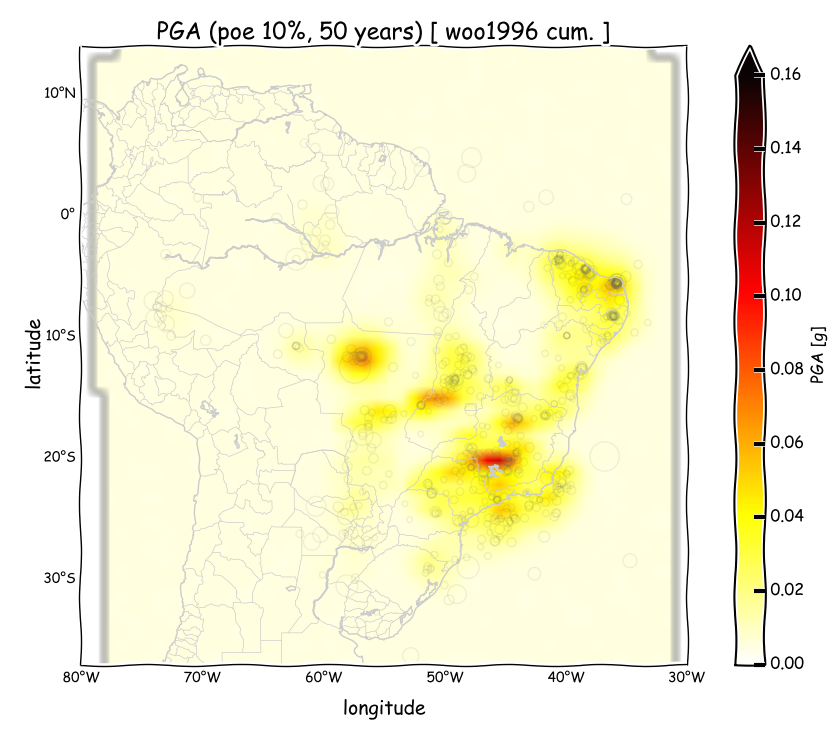
\includegraphics[height=0.95\textheight]{pga_woo_cum} 
	\caption{Mapa de ameaça sísmica, PGA (poe 10\%, 50y).}
	\label{fig:pga_woo_cum} 
\end{figure}
\end{frame}



%-----------------------------------------------------------------------------
\begin{frame}{Woo1996: Ameaça (diferença)}
\begin{figure}[H]
	\centering
		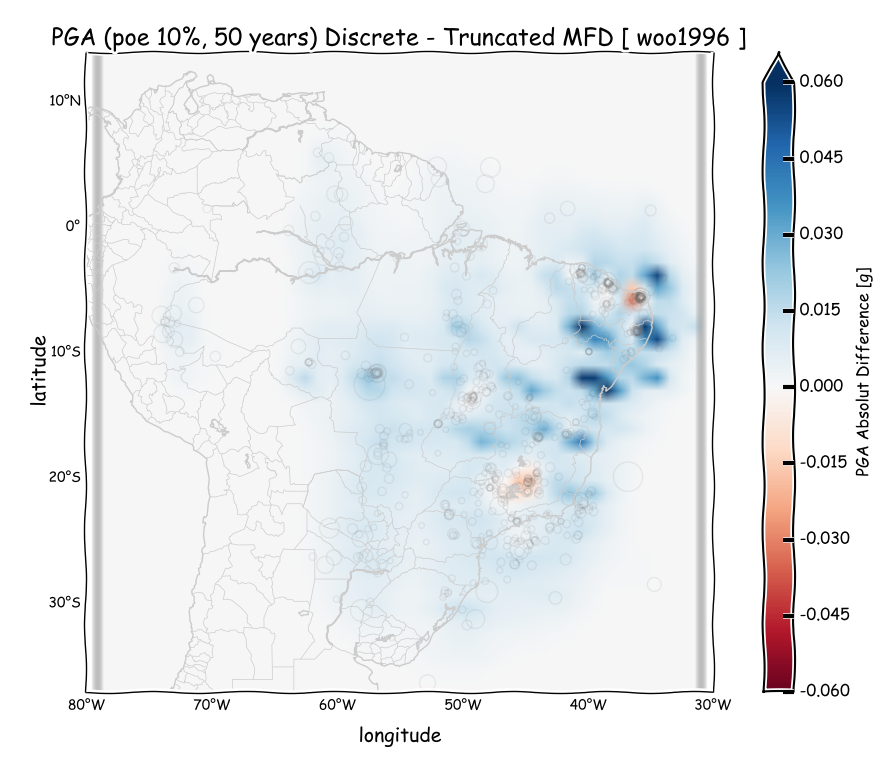
\includegraphics[height=0.95\textheight]{pga_woo_dif} 
		\caption{Mapa diferencial de ameaça, PGA (poe 10\%, 50y)
		   entre os mapas das figuras 
		   \ref{fig:pga_woo_inc} e \ref{fig:pga_woo_cum}.}
		\label{fig:pga_woo_dif} 
\end{figure}
\end{frame}



%=============================================================================
\subsection{Helmstetter, 2012}
%=============================================================================


%-----------------------------------------------------------------------------
\begin{frame}{Helmstetter2012: Catálogos de treinamento e de teste}
\begin{figure}[H]
  \centering
  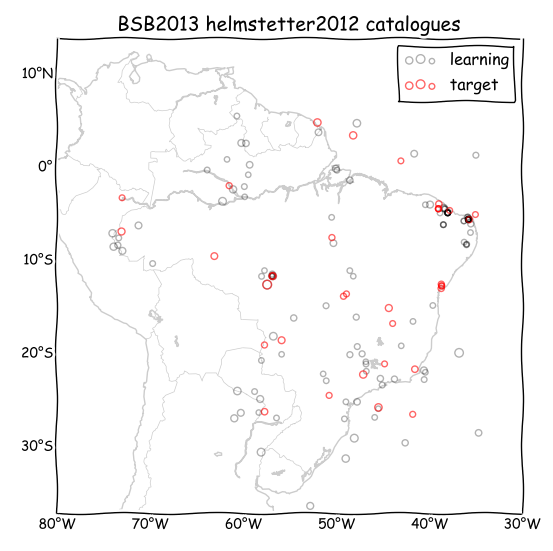
\includegraphics[height=.90\textheight]{helmstetter_catalogues} 
  \caption{Catálogos de aprendizado e de teste para o método de \citet{helmstetter_2012}}
  \label{fig:h_catalogue} 
\end{figure}
\end{frame}



%-----------------------------------------------------------------------------
\begin{frame}{Helmstetter2012: Larguras de banda}
\begin{figure}[H]
  \centering
  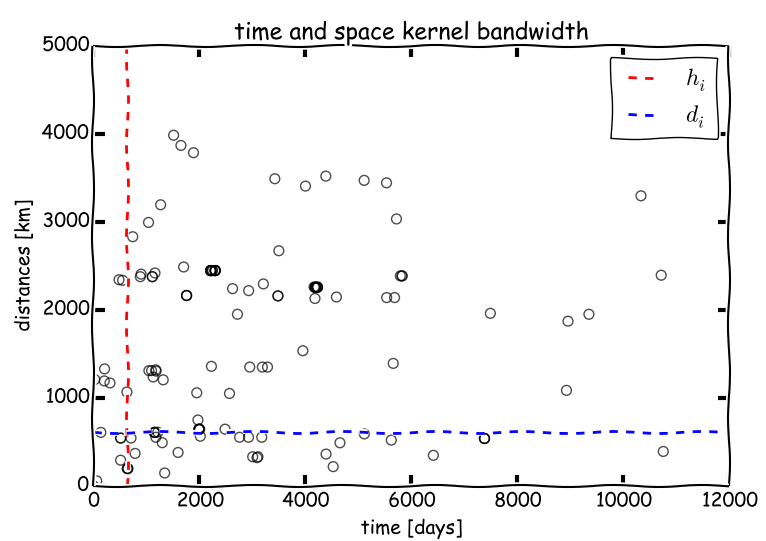
\includegraphics[height=.90\textheight]{helmstetter_hidi} 
  \caption{Exemplo da largura de banda para um determinado evento para o método de Helmstetter, com $k_{cnn} = 5$ e
  $a_{cnn} = 100$}
  \label{fig:h_hidi} 
\end{figure}
\end{frame}



%-----------------------------------------------------------------------------
\begin{frame}{Helmstetter2012: Taxa estacionária de sismicidade}
\begin{figure}[H]
  \centering
  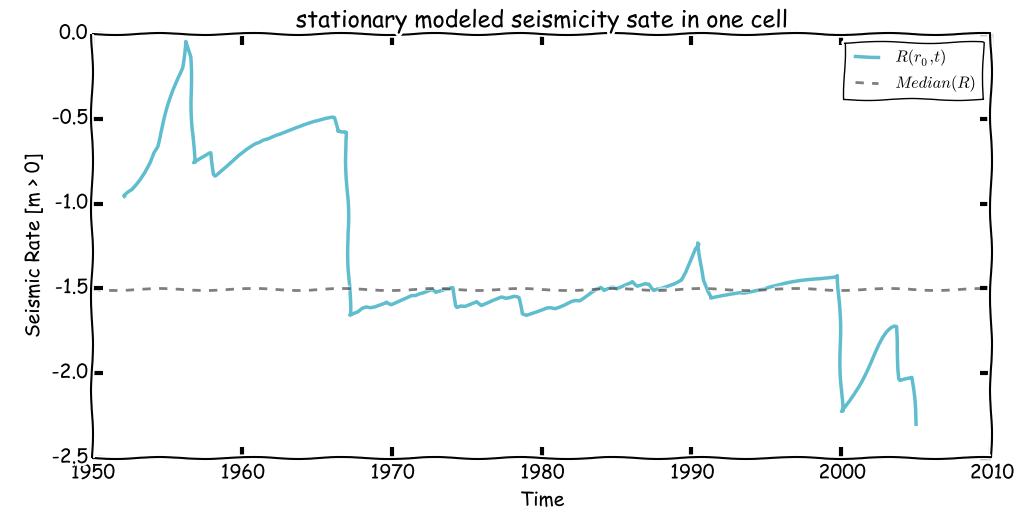
\includegraphics[width=.90\textwidth]{helmstetter_stationary_a} 
  \caption{Taxa de sismicidade estacionaria calculada a partir da mediana da
  taxa de sismicidade modelada pelo método de Helmstetter2012 para uma determinada célula $r_0$}
  \label{fig:h_stationary} 
\end{figure}
\end{frame}



%-----------------------------------------------------------------------------
\begin{frame}{Helmstetter2012: Parâmetros otimizados}
\begin{table}[H]
	\centering
	\begin{tabular}{c|c}
		Parâmetro & Valor \\ \hline
		$R_{min}$ & $0.1\times10^{-13}$ \\
		$a_{cnn}$ & 325 \\
		$k_{cnn}$ & 1 \\
	\end{tabular}
	\caption{Parâmetros otimizados para o modelo de Helmstetter a partir do catálogo \gls{bsb2013}}
	\label{tab:hemlstetter}
\end{table}
\end{frame}


%-----------------------------------------------------------------------------
\begin{frame}{Helmstetter2012: Taxa de sismicidade}
\begin{figure}[H]
  \centering
  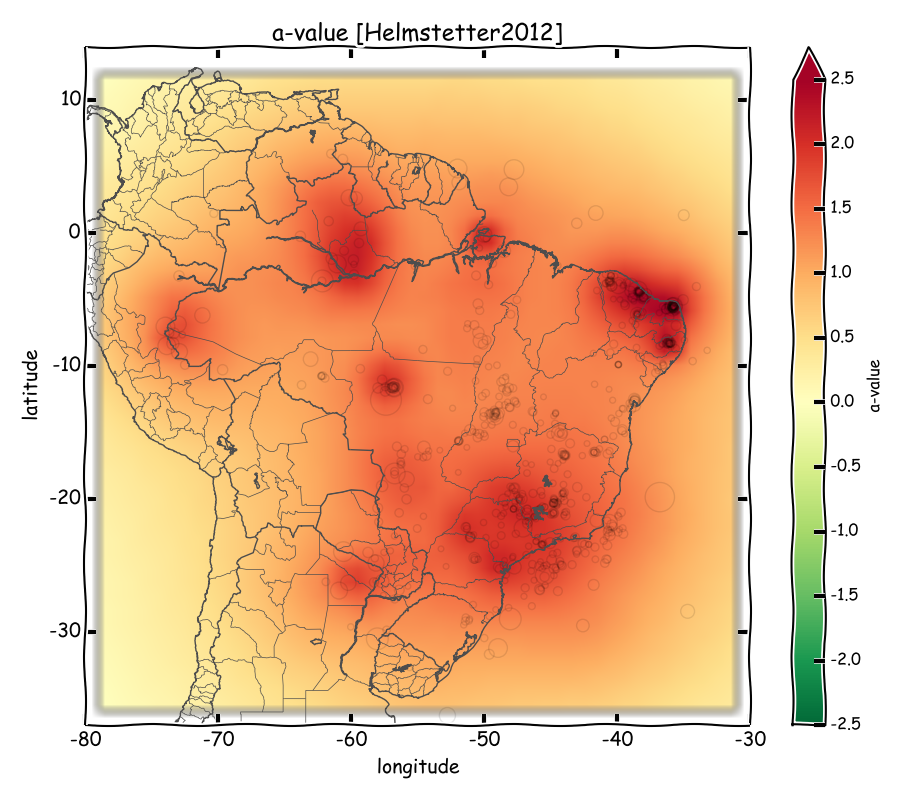
\includegraphics[height=.95\textheight]{a_helmstetter} 
  \caption{Mapa do valor-a, usando o catálogo \gls{bsb2013} calculado pelo método de Helmstetter, 2012 }
  \label{fig:helm_r} 
\end{figure}
\end{frame}


%-----------------------------------------------------------------------------
\begin{frame}{Helmstetter2012: Ameaça}
\begin{figure}[H]
  \centering
  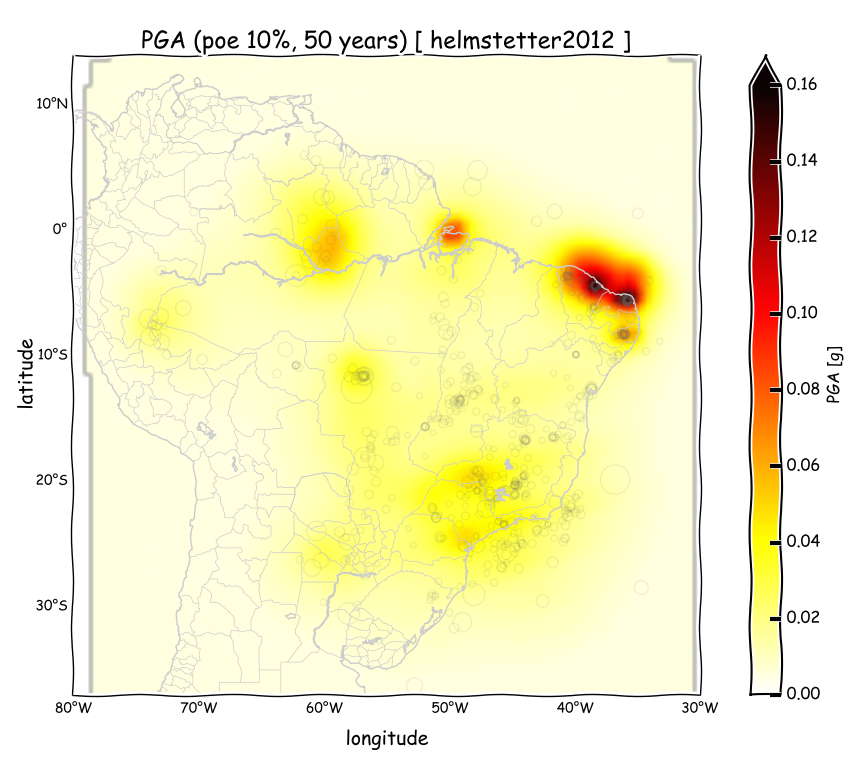
\includegraphics[height=.93\textheight]{pga_helmstetter} 
  \caption{Mapa de ameaça sísmica, PGA (poe 10\%, 50y), 
  		   calculado com o OpenQuake a partir das fontes sísmicas
  		   determinas pelo método de Helmstetter,2012 }
  \label{fig:helm_h} 
\end{figure}
\end{frame}




%=============================================================================
\section{Discussão}
%=============================================================================
%-----------------------------------------------------------------------------
\begin{frame}{slide}




\end{frame}




%=============================================================================
\subsection{Contribuições}
%=============================================================================
%-----------------------------------------------------------------------------
\begin{frame}{slide}


\end{frame}



%=============================================================================
\subsection{Melhorias futuras}
%=============================================================================
%-----------------------------------------------------------------------------
\begin{frame}{slide}


\end{frame}



%-----------------------------------------------------------------------------
\begin{frame}{slide}


\end{frame}



%-----------------------------------------------------------------------------
\begin{frame}{slide}


\end{frame}



%-----------------------------------------------------------------------------
\begin{frame}{slide}


\end{frame}



%-----------------------------------------------------------------------------
\begin{frame}{slide}


\end{frame}



%-----------------------------------------------------------------------------
\begin{frame}{slide}


\end{frame}



%-----------------------------------------------------------------------------
\begin{frame}{slide}


\end{frame}



%-----------------------------------------------------------------------------
\begin{frame}{slide}


\end{frame}



%-----------------------------------------------------------------------------
\begin{frame}{slide}


\end{frame}




\begin{frame}{Make Titles Informative. Use Uppercase Letters. Long Titles are Split Automatically.}{Subtitles are optional.}
  % - A title should summarize the slide in an understandable fashion
  %   for anyone how does not follow everything on the slide itself.

	\begin{figure}[H]
	  \centering
	  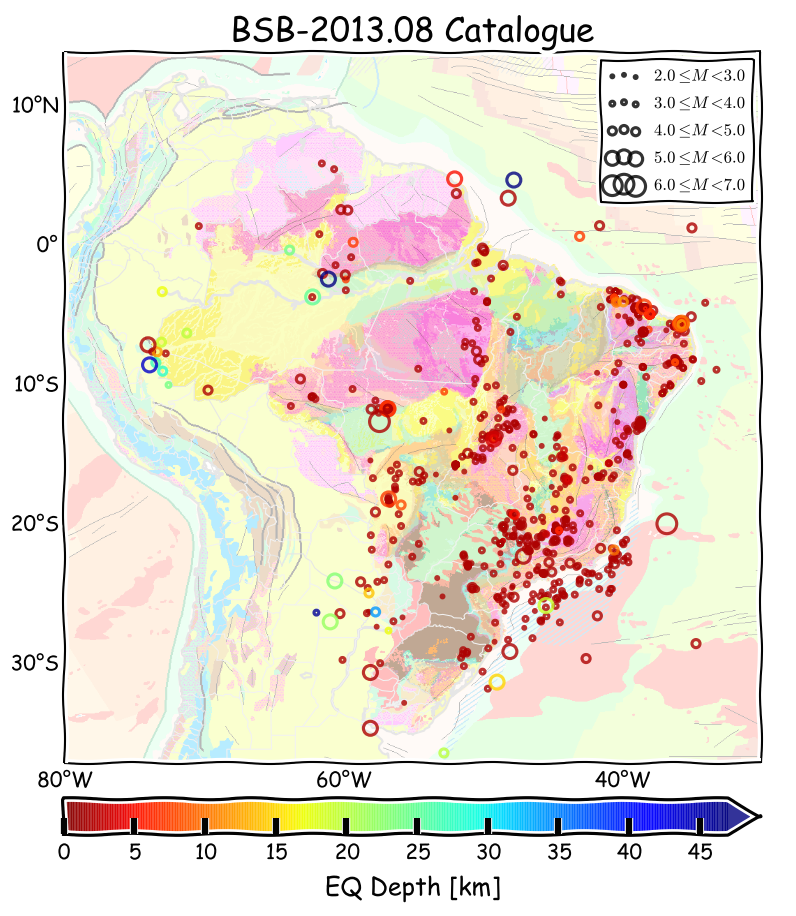
\includegraphics[height=.90\textheight]{seismicity_br} 
	  \caption{Sismicidade do Brasil. Catálogo \gls{bsb2013}.}
	  \label{fig:br_seis} 
	\end{figure}


\end{frame}


\begin{frame}{Figura teste}
explicar algum item por exemplo
	\begin{itemize}
		\item algum argumento pra dar
	\end{itemize}
	\begin{figure}[H]
		\centering{}
		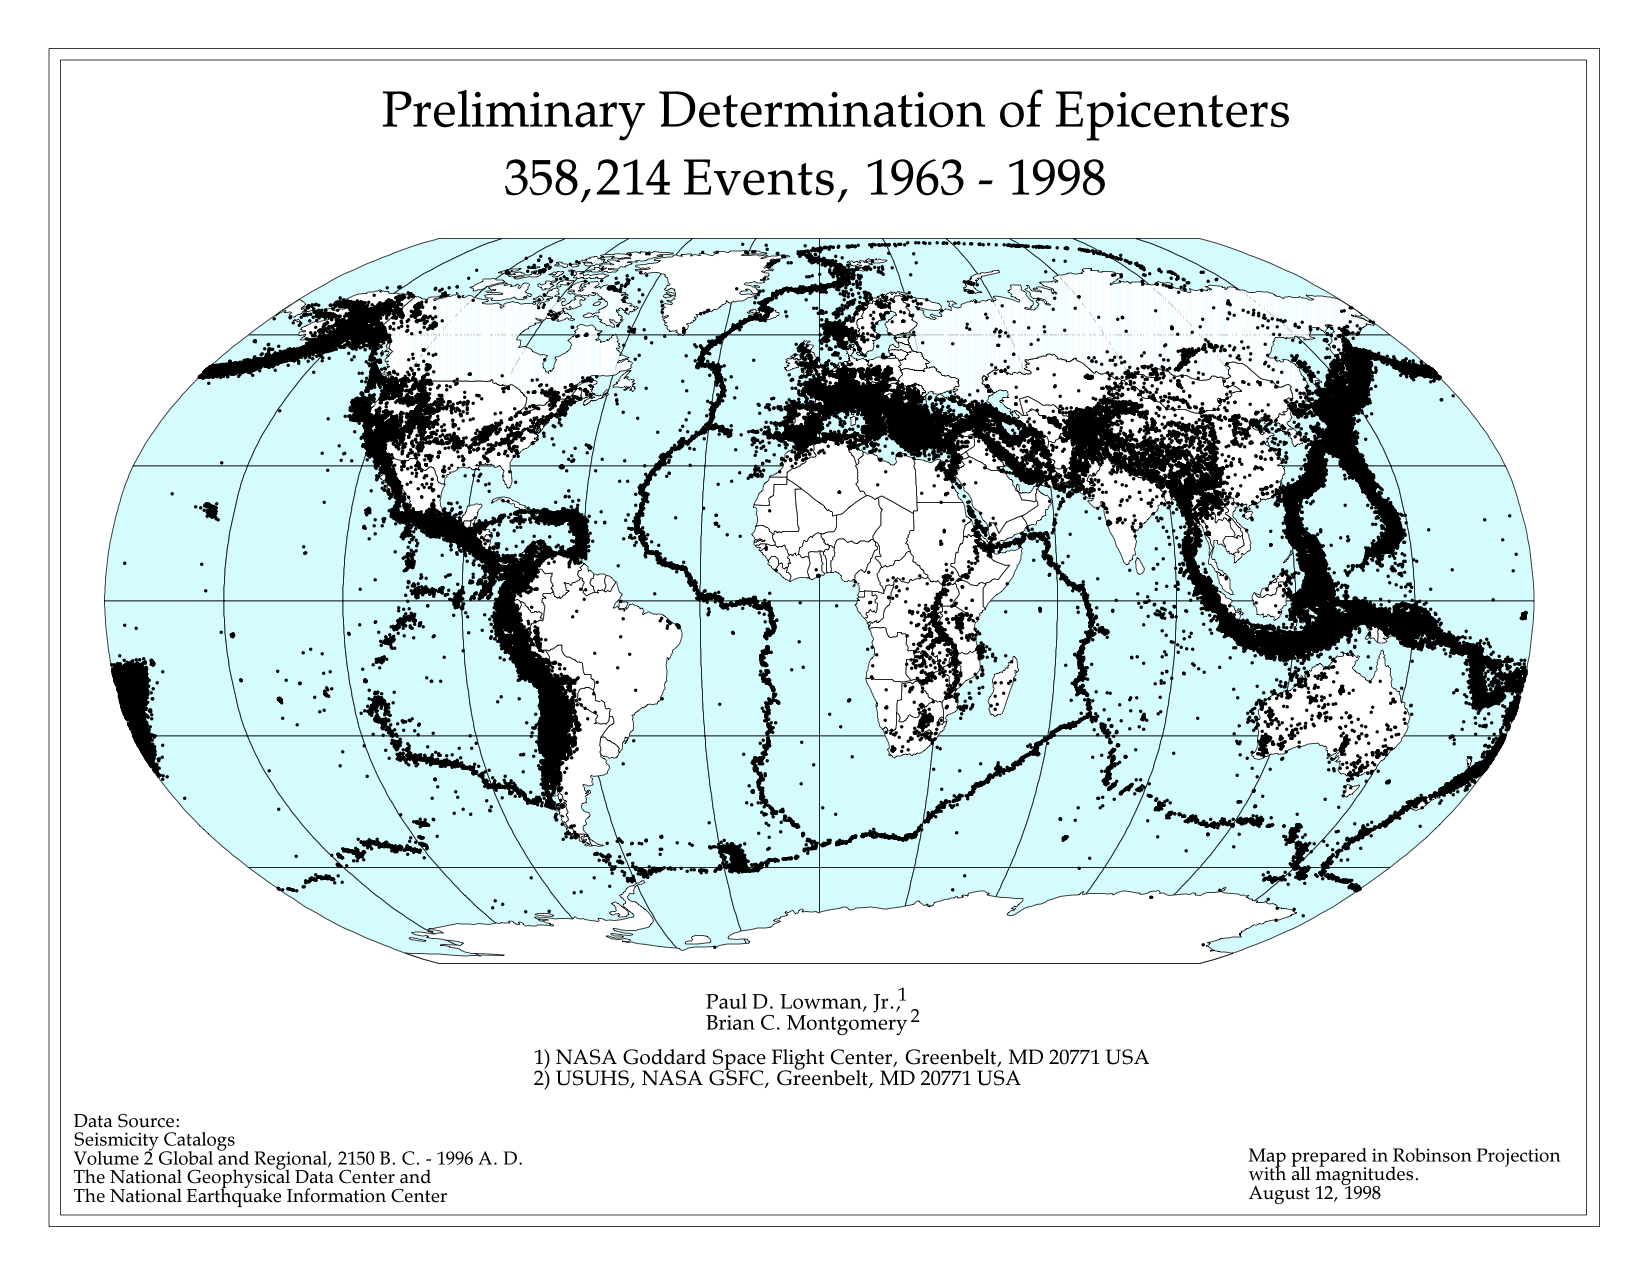
\includegraphics[height=0.70\textheight]{global_pde_mag_all}
		\caption[Mapa Mundial de Epicentros 1963-1998]
		{Mapa Mundial de Epicentros 1963-1998 \citet{lowman_jr_1998}}
		\label{f:global_epicenters}
\end{figure}
\end{frame}



%
\begin{frame}{Figura teste}
explicar algum item por exemplo
\begin{itemize}
	\item algum argumento pra dar
\end{itemize}

\begin{figure}[H]
   \centering
   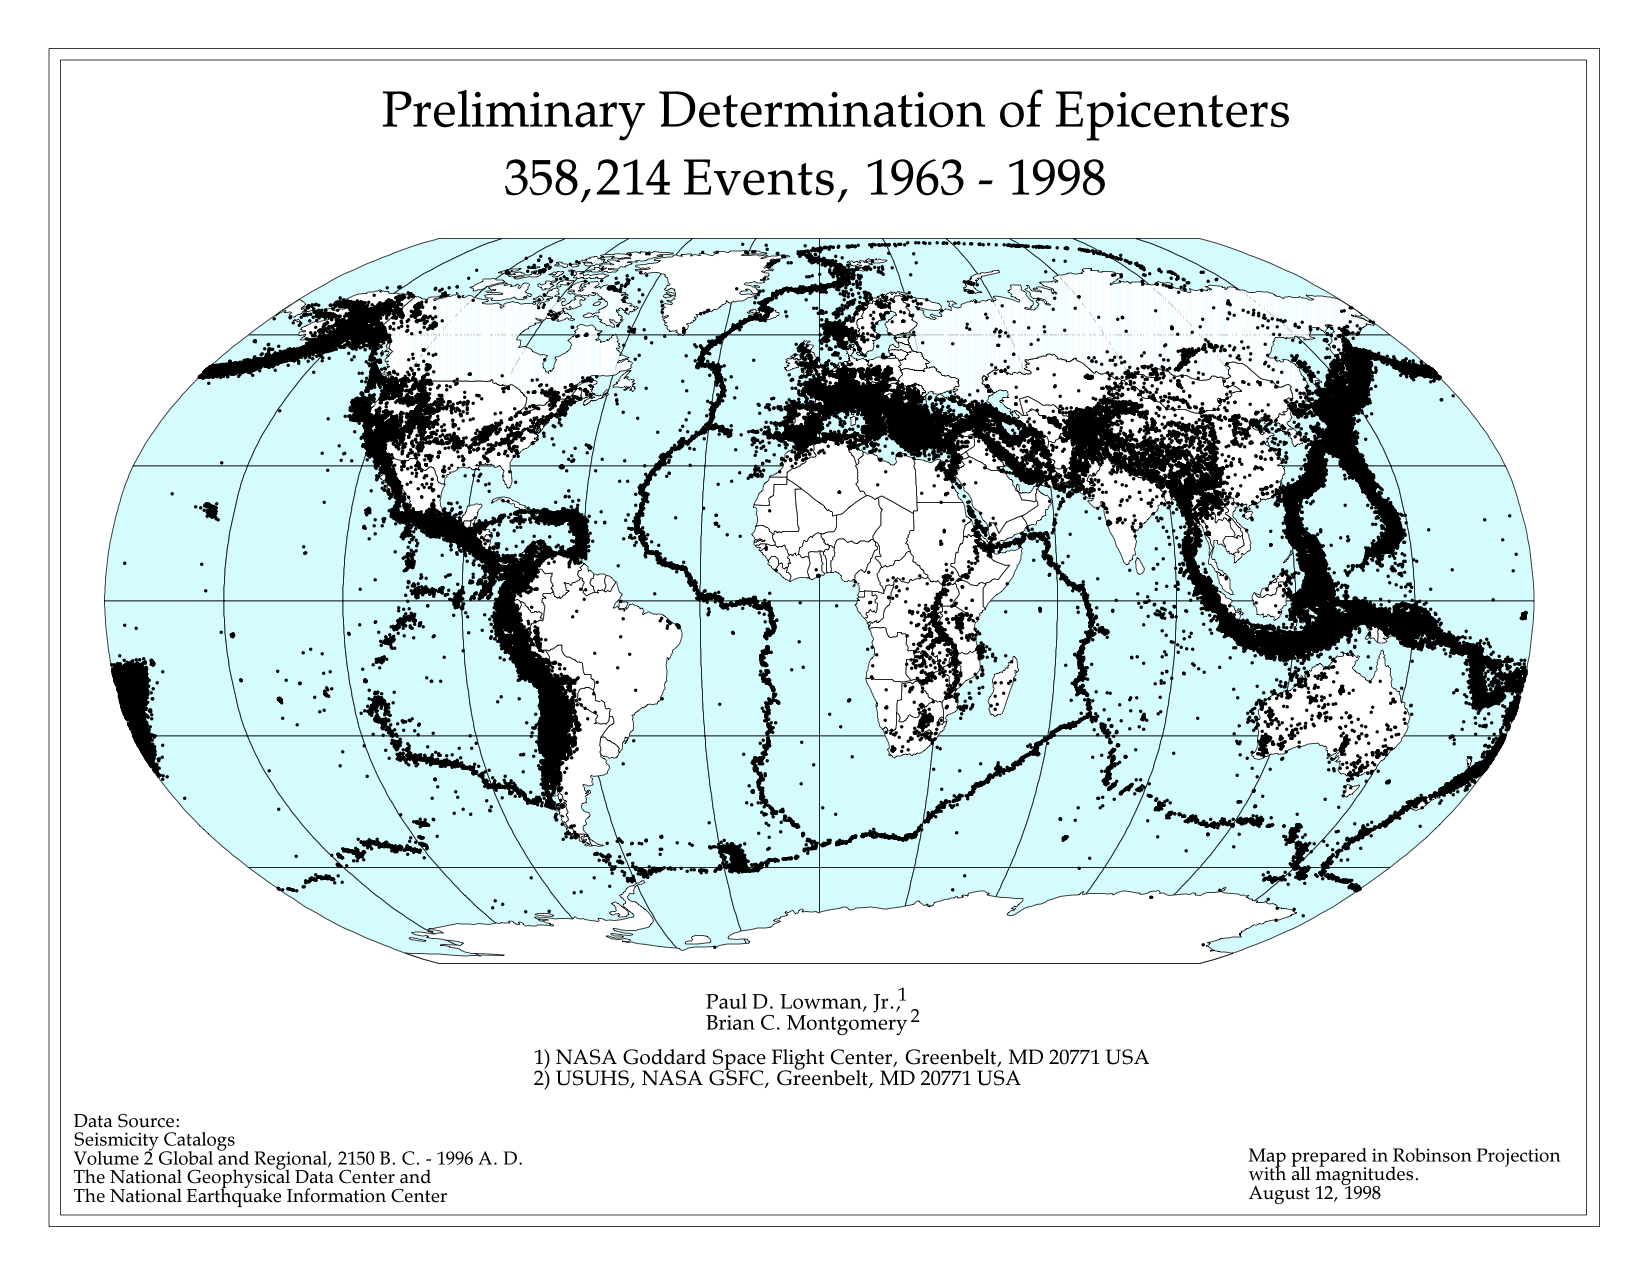
\includegraphics[height=0.70\textheight]{global_pde_mag_all}
   \caption[Mapa Mundial de Epicentros 1963-1998]
   		   {Mapa Mundial de Epicentros 1963-1998 \citet{lowman_jr_1998} } 
   \label{f:global_epicenters}
\end{figure}
\end{frame}


\begin{frame}{Subfiguras outro teste}
se eu disser algo por aqui dá zica \\
testa pra ver
\begin{figure}
	\centering
	\begin{subfigure}[t]{0.48\textheight}
		  	\centering
			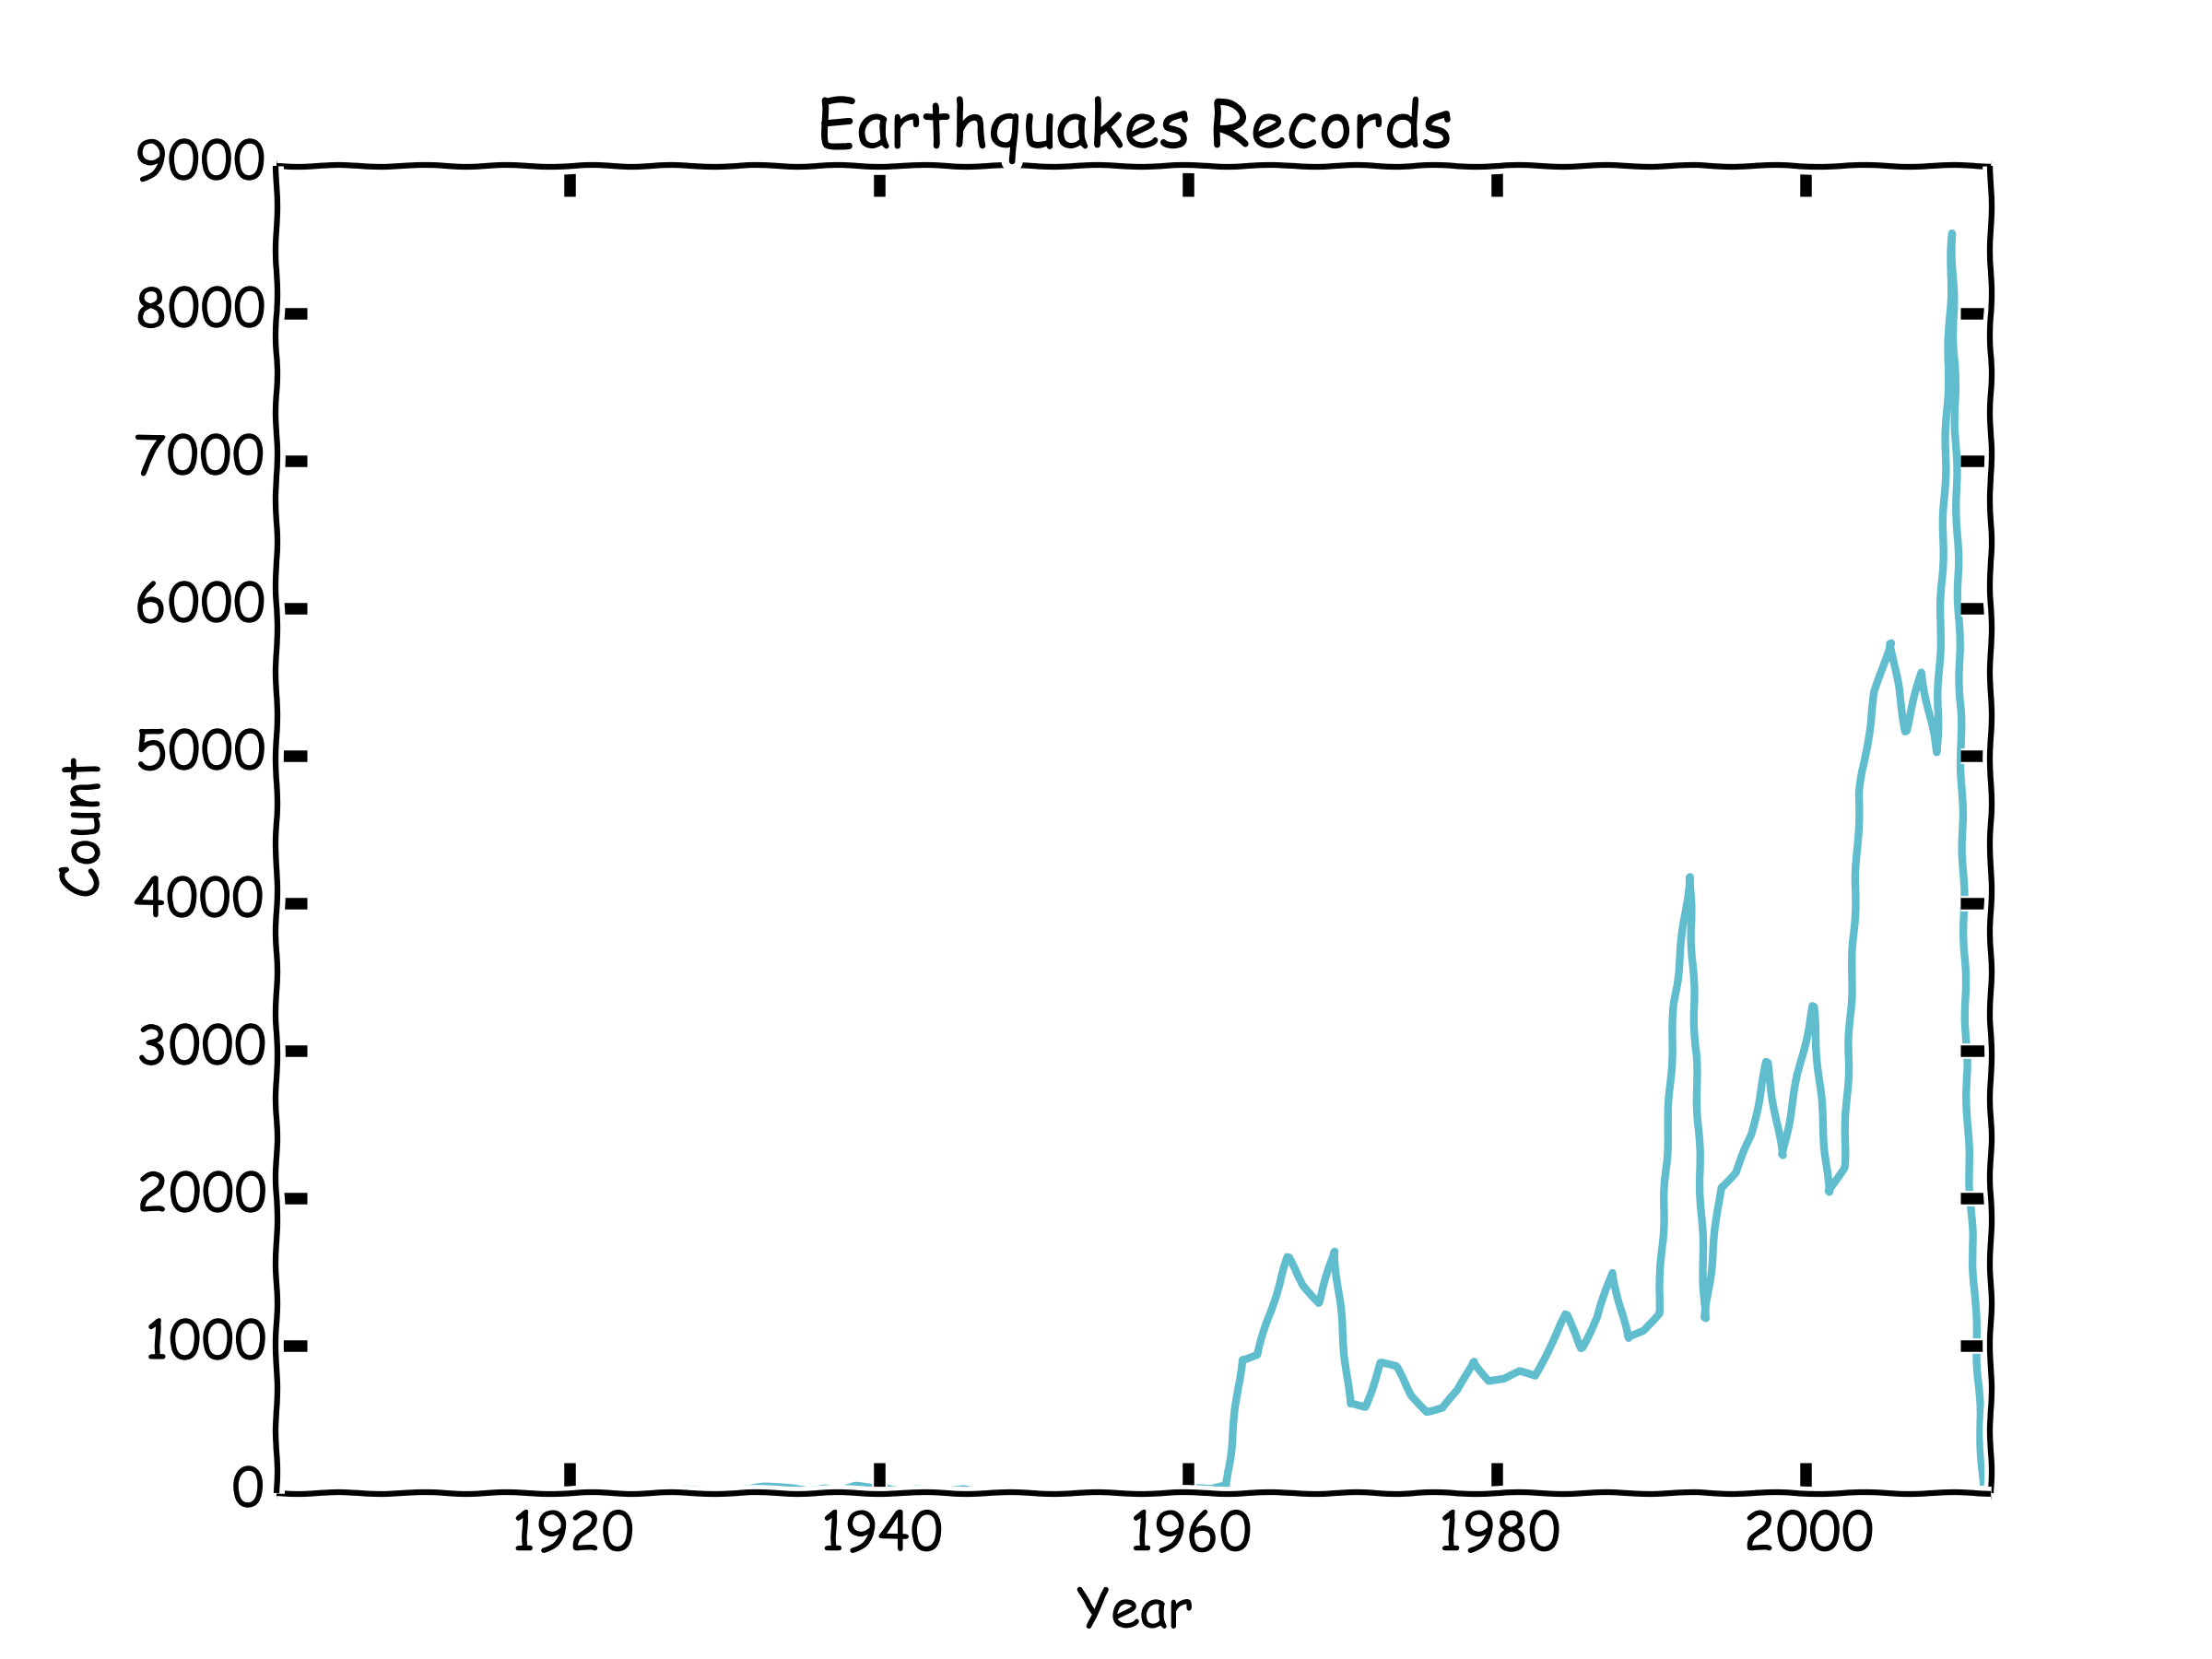
\includegraphics[height=1.00\textheight]{hmtk_sa3_rate}
			\subcaption{Número de tremores registrados por ano, \gls{iscgem}}
			\label{fig:sa_eq_record}
	\end{subfigure}%
	\quad %~ %add desired spacing between images, e. g. ~, \quad, \qquad, \hfill etc.
	\begin{subfigure}[t]{0.48\textheight}
		  	\centering
			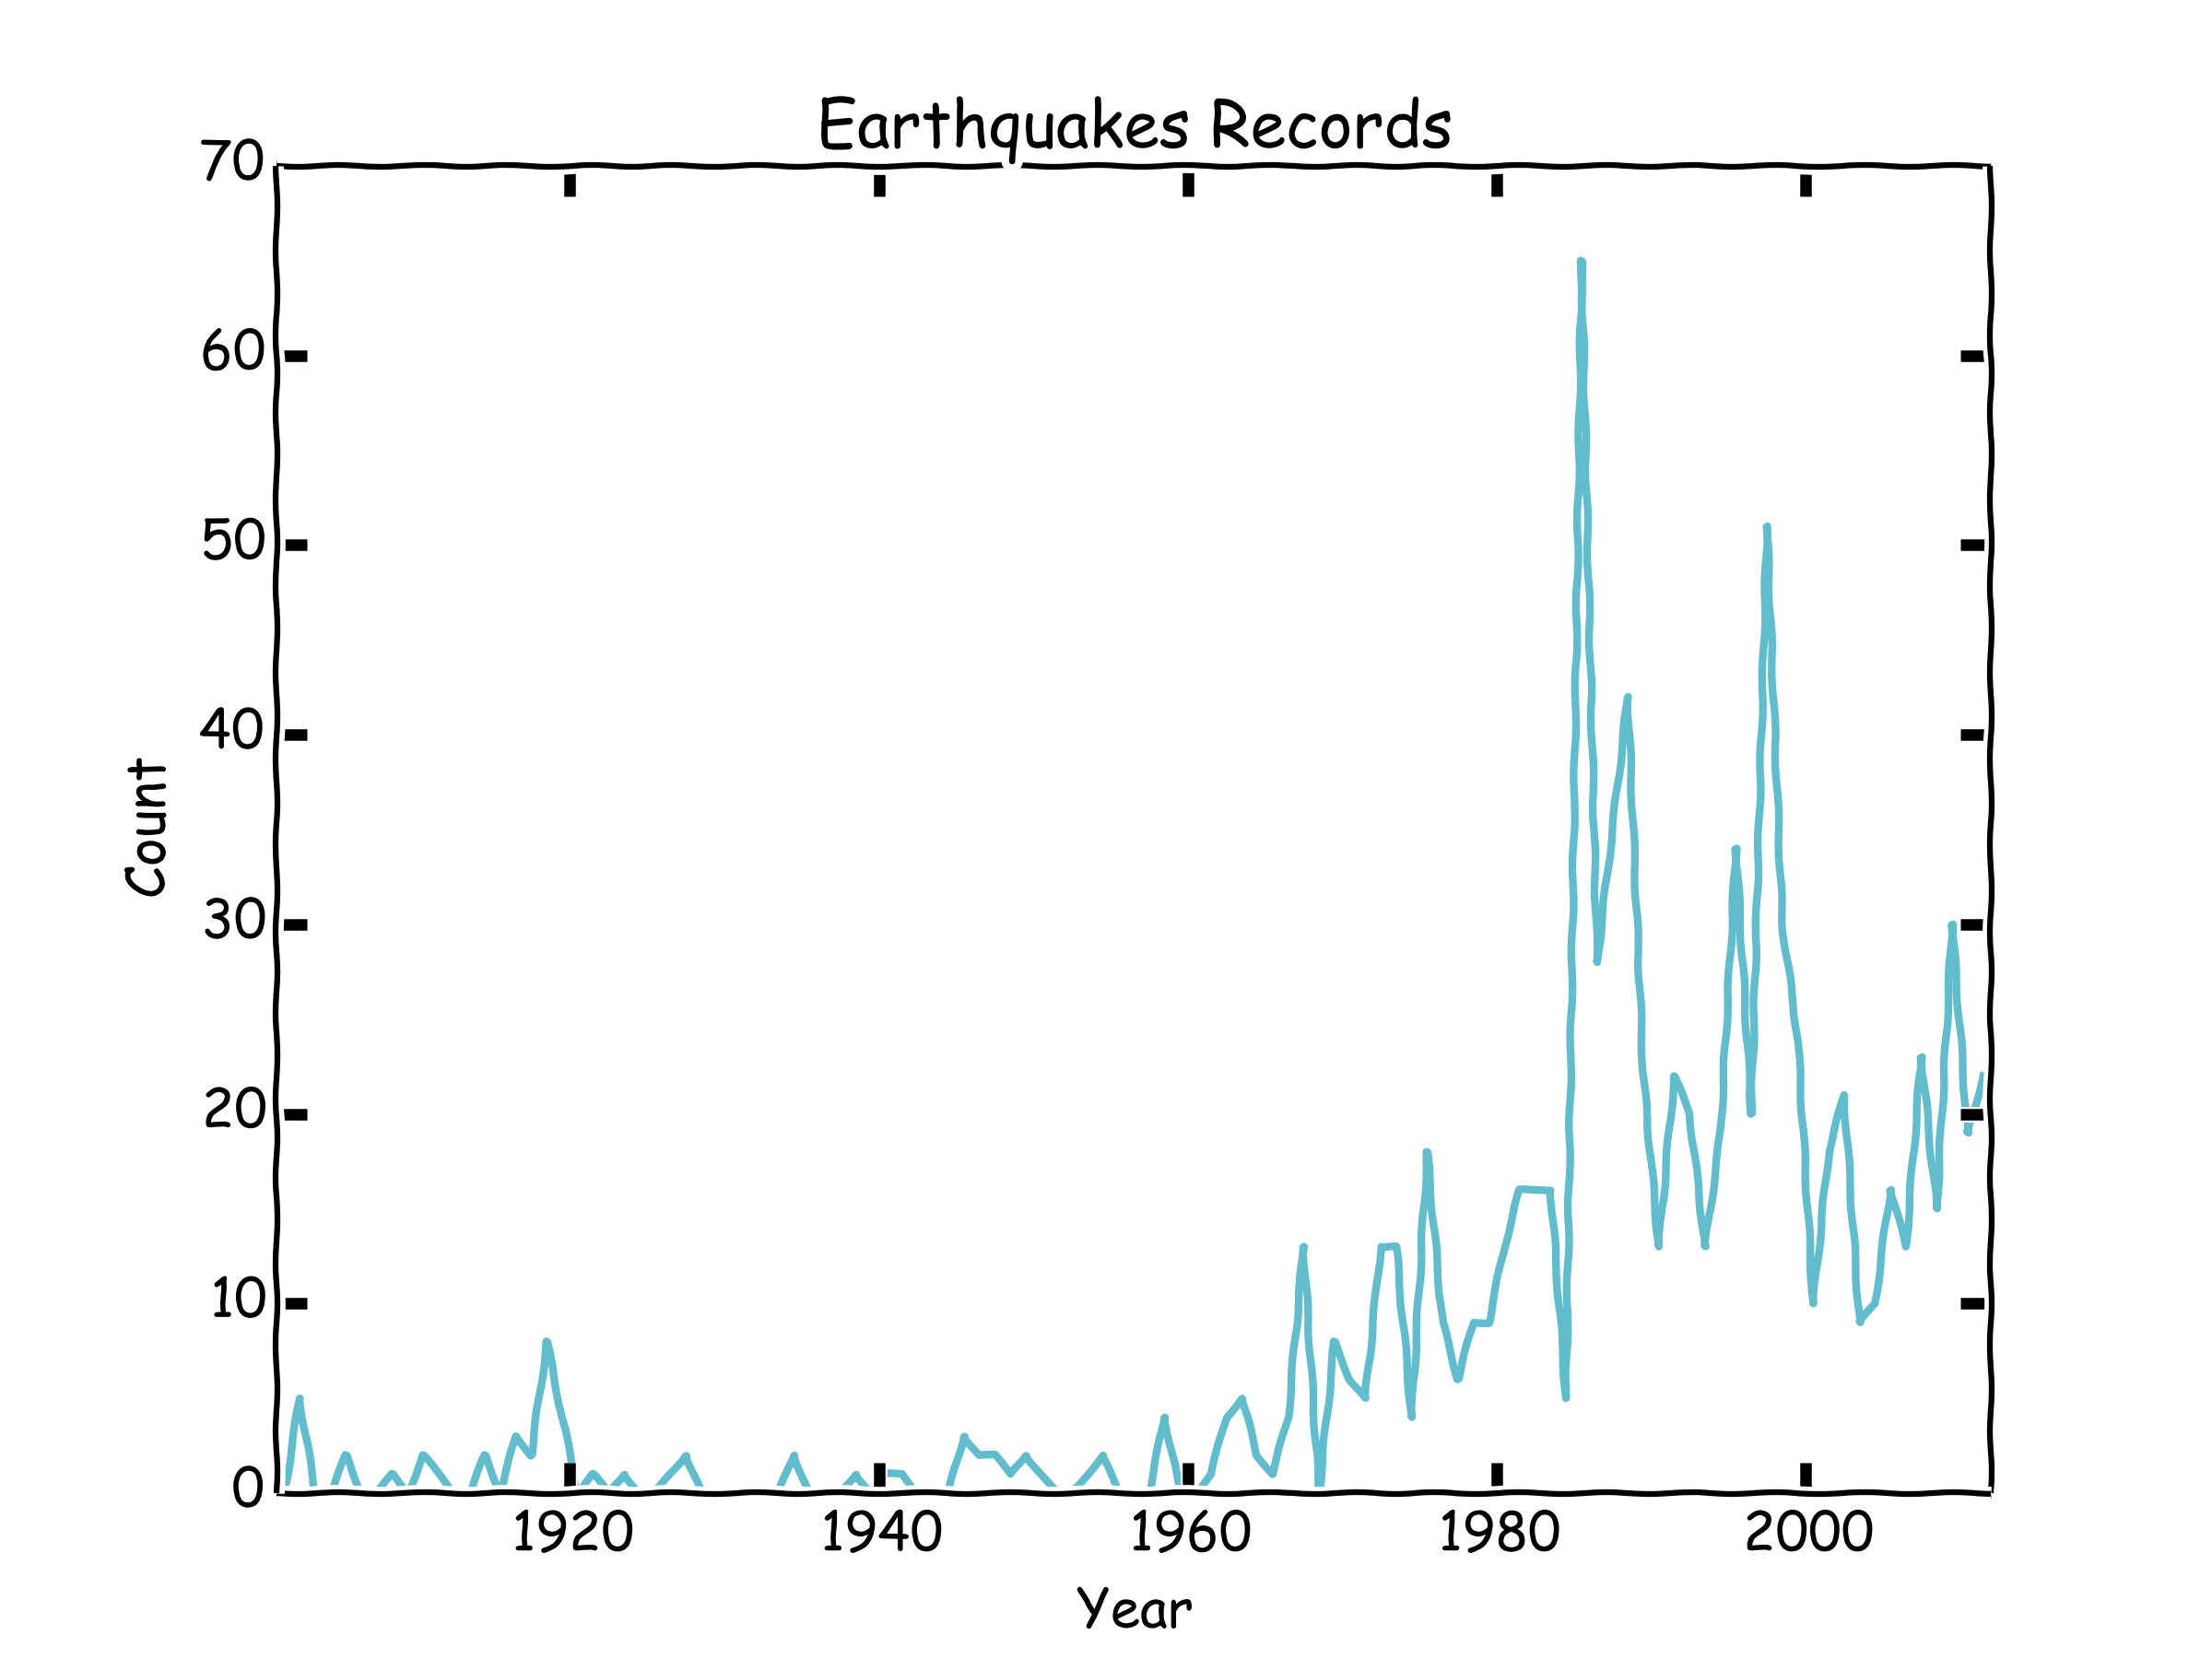
\includegraphics[height=1.00\textheight]{hmtk_bsb2013_rate}
			\subcaption{Número de tremores registrados por ano, \gls{bsb2013}}
			\label{fig:br_eq_record}
    \end{subfigure}
	\caption{Número de tremores registrados por ano após 1900}
	\label{fig:eq_record}
\end{figure}
\end{frame}



\begin{frame}{Make Titles Informative.}

  You can create overlays\dots
  \begin{itemize}
  \item using the \texttt{pause} command:
    \begin{itemize}
    \item
      First item.
      \pause
    \item    
      Second item.
    \end{itemize}
  \item
    using overlay specifications:
    \begin{itemize}
    \item<3->
      First item.
    \item<4->
      Second item.
    \end{itemize}
  \item
    using the general \texttt{uncover} command:
    \begin{itemize}
      \uncover<5->{\item
        First item.}
      \uncover<6->{\item
        Second item.}
    \end{itemize}
  \end{itemize}
\end{frame}



\begin{frame}{Subfiguras outro teste}
\begin{figure}
	\centering
	\begin{subfigure}[b]{0.48\textheight}
		  	\centering
			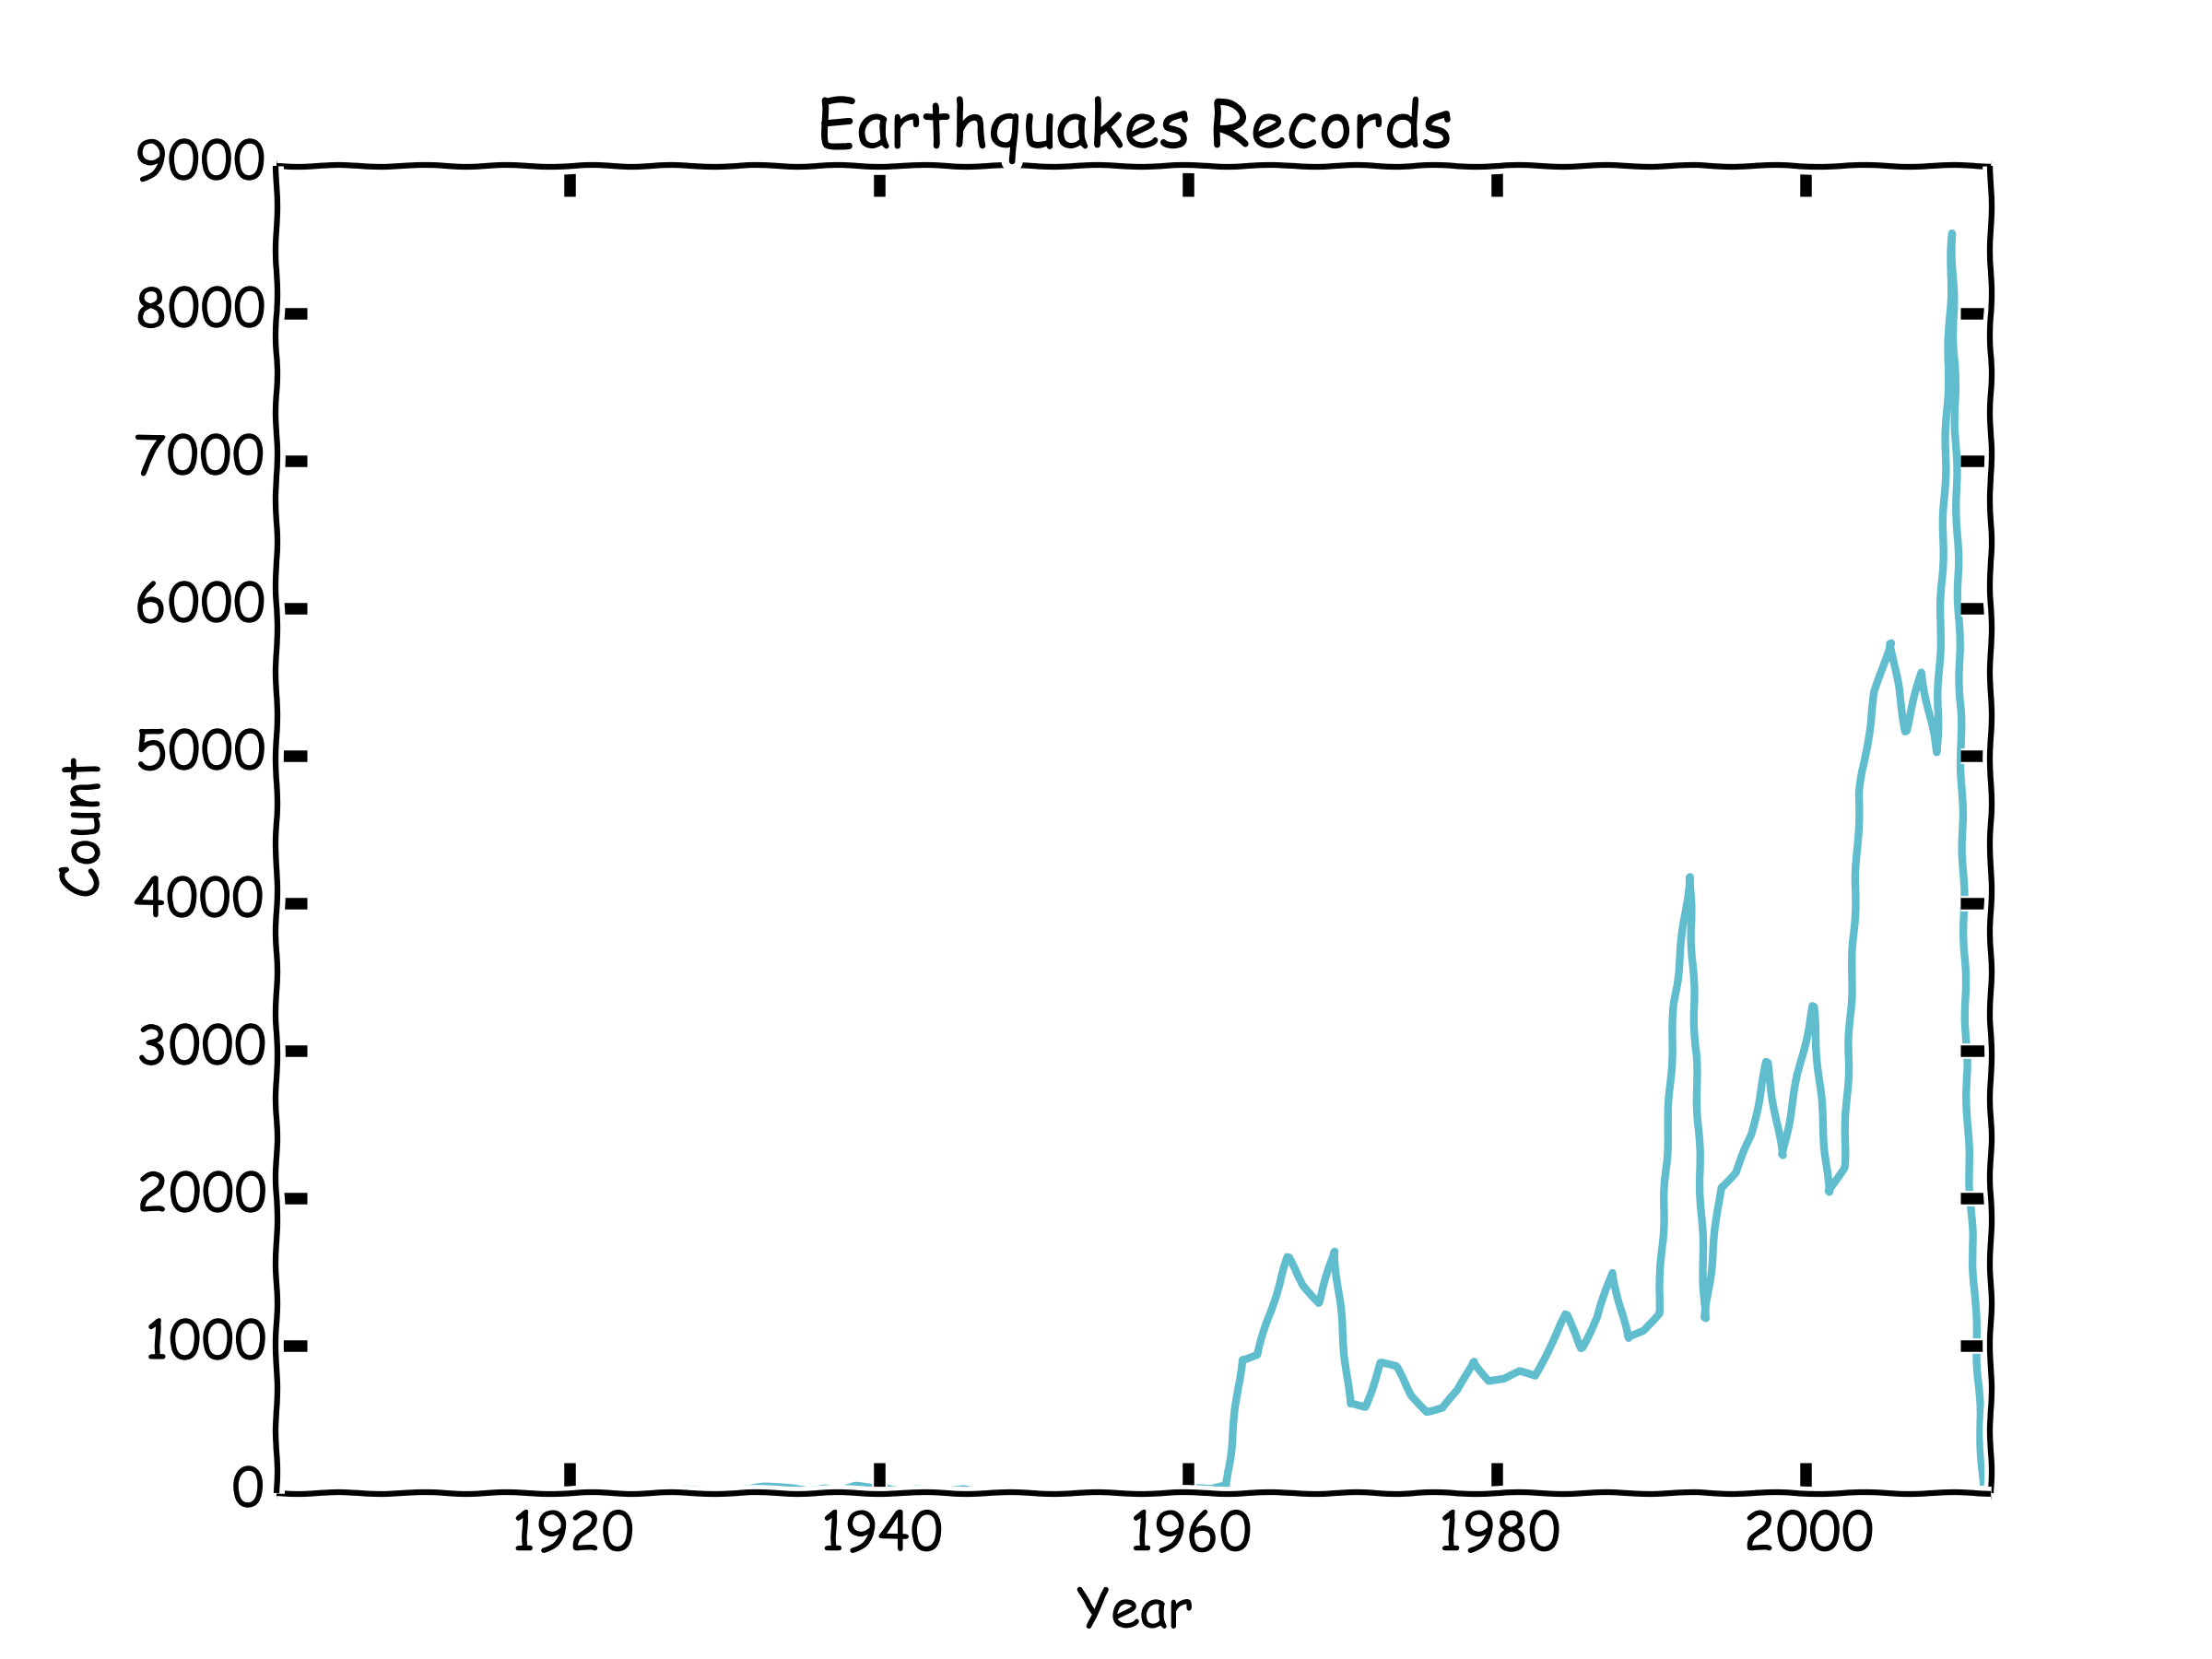
\includegraphics[height=1.00\textheight]{hmtk_sa3_rate}
			\subcaption{Número de tremores registrados por ano, \gls{iscgem}}
			\label{fig:sa_eq_record}
	\end{subfigure}%
	\quad %~ %add desired spacing between images, e. g. ~, \quad, \qquad, \hfill etc.
	\begin{subfigure}[b]{0.48\textheight}
		  	\centering
			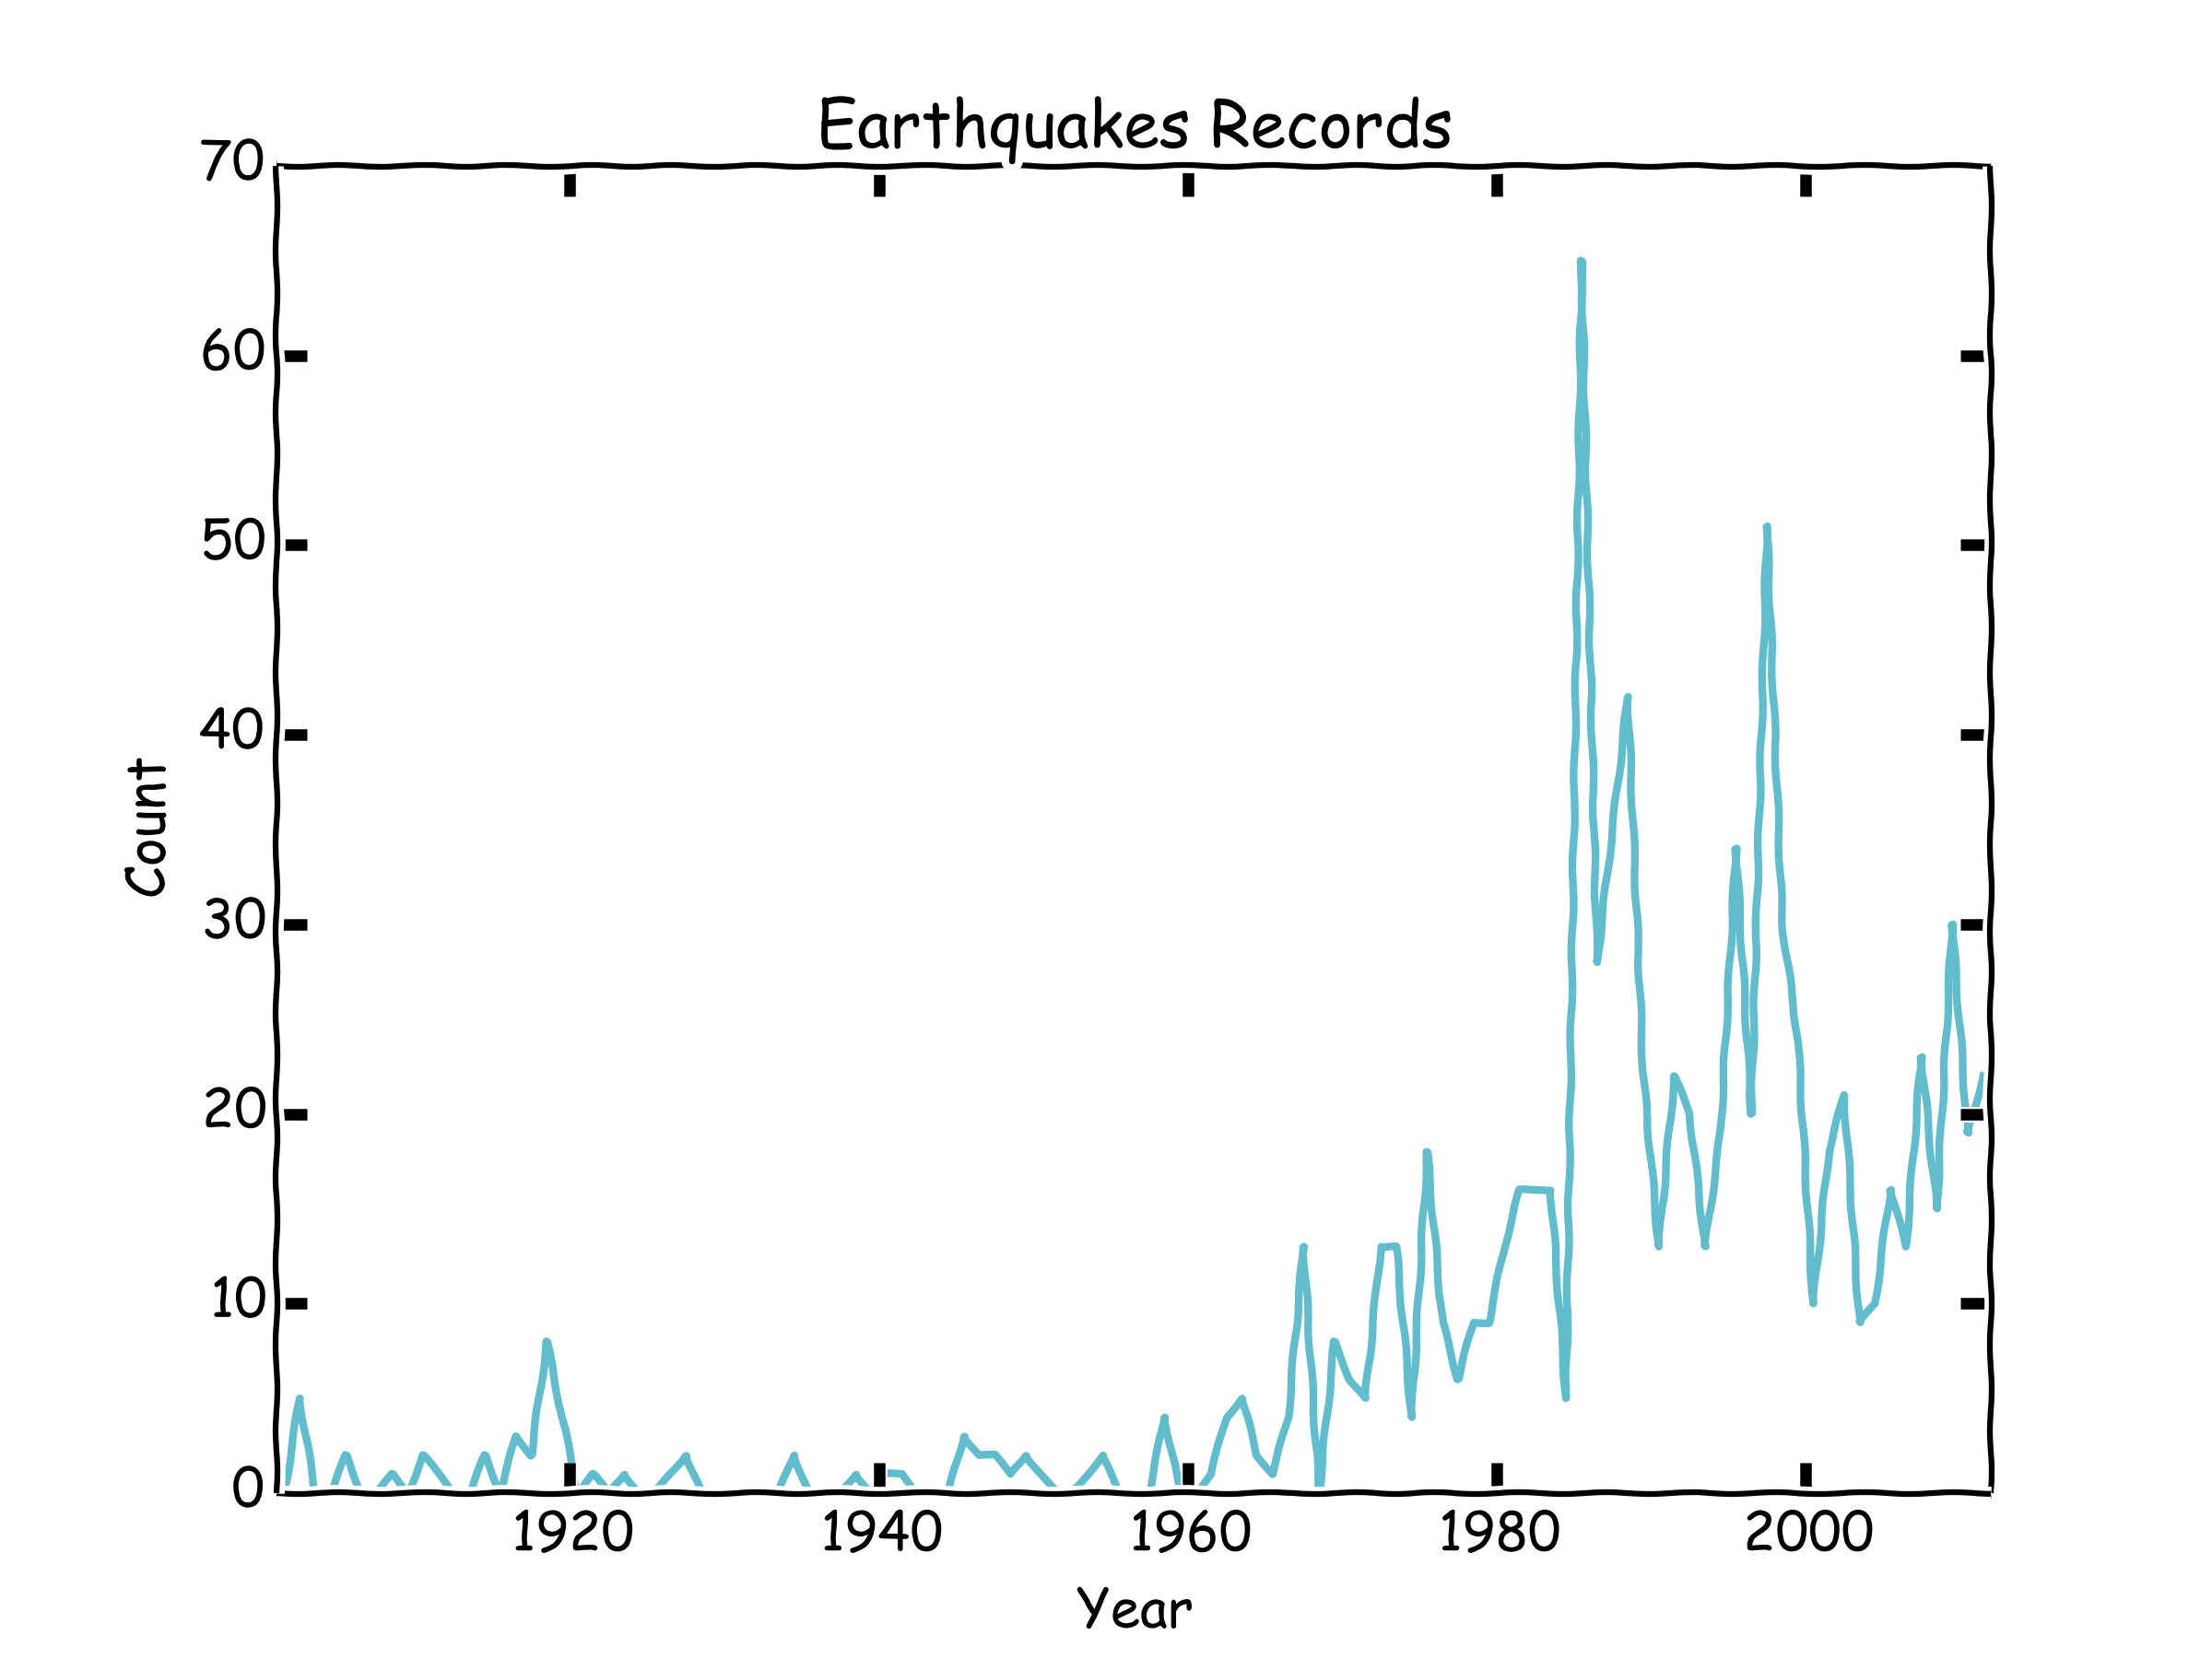
\includegraphics[height=1.00\textheight]{hmtk_bsb2013_rate}
			\subcaption{Número de tremores registrados por ano, \gls{bsb2013}}
			\label{fig:br_eq_record}
    \end{subfigure}
	\caption{Número de tremores registrados por ano após 1900}
	\label{fig:eq_record}
\end{figure}
\end{frame}

%\subsection{Previous Work}

\begin{frame}[fragile]{An old algorithm}
% NB. listings is quite powerful, but not well suited to be used with beamer
%  consider using semiverbatim or the like, see below
\begin{lstlisting}[language=C]
int main (void)
{
  std::vector<bool> is_prime (100, true);
  for (int i = 2; i < 100; i++)
    if (is_prime[i])
      {
        std::cout << i << " ";
        for (int j = i; j < 100;
            is_prime [j] = false, j+=i);
      }
  return 0;
}
\end{lstlisting}
\end{frame}

\begin{frame}[fragile]
  \frametitle{An Algorithm For Finding Primes Numbers.}
\begin{semiverbatim}
\uncover<1->{\alert<0>{int main (void)}}
\uncover<1->{\alert<0>{\{}}
\uncover<1->{\alert<1>{ \alert<4>{std::}vector<bool> is_prime (100, true);}}
\uncover<1->{\alert<1>{ for (int i = 2; i < 100; i++)}}
\uncover<2->{\alert<2>{    if (is_prime[i])}}
\uncover<2->{\alert<0>{      \{}}
\uncover<3->{\alert<3>{        \alert<4>{std::}cout << i << " ";}}
\uncover<3->{\alert<3>{        for (int j = i; j < 100;}}
\uncover<3->{\alert<3>{             is_prime [j] = false, j+=i);}}
\uncover<2->{\alert<0>{      \}}}
\uncover<1->{\alert<0>{ return 0;}}
\uncover<1->{\alert<0>{\}}}
\end{semiverbatim}
  \visible<4->{Note the use of \alert{\texttt{std::}}.}
\end{frame}

%\section{Our Results/Contribution}
%\subsection{Main Results}

\begin{frame}{Make Titles Informative.}
  \begin{example}
    \begin{itemize}
    \item 2 is prime (two divisors: 1 and 2).
    \item 3 is prime (two divisors: 1 and 3).
    \item 4 is not prime (\alert{three} divisors: 1, 2, and 4).
    \end{itemize}
  \end{example}
\end{frame}

\begin{frame}{Make Titles Informative.}
\begin{theorem}
 There is no largest prime number and, in addition, $$\int_\Omega \nabla u \cdot \nabla v = - \int_\Omega u \Delta v + \int_{\partial\Omega} u v n$$
 \end{theorem}
 \begin{proof}
 \begin{enumerate}
 \item<1-> Suppose $p$ were the largest prime number.
 \item<2-> Let $q$ be the product of the first $p$ numbers.
 \item<3-> Then $q + 1$ is not divisible by any of them.
 \item<1-> Thus $q + 1$ is also prime and greater than $p$.\qedhere
 \end{enumerate} 
 \end{proof}
 \uncover<4->{The proof used \textit{reductio ad absurdum}.}
\end{frame}

\begin{frame}{Make Titles Informative.}
\end{frame}


%\subsection{Basic Ideas for Proofs/Implementation}

\begin{frame}{Make Titles Informative.}
\end{frame}

\begin{frame}{Make Titles Informative.}
\end{frame}

\begin{frame}{Make Titles Informative.}
\end{frame}



\section*{Summary}

\begin{frame}{Summary}

  % Keep the summary *very short*.
  \begin{itemize}
  \item
    The \alert{first main message} of your talk in one or two lines.
  \item
    The \alert{second main message} of your talk in one or two lines.
  \item
    Perhaps a \alert{third message}, but not more than that.
  \end{itemize}
  
  % The following outlook is optional.
  \vskip0pt plus.5fill
  \begin{itemize}
  \item
    Outlook
    \begin{itemize}
    \item
      Something you haven't solved.
    \item
      Something else you haven't solved.
    \end{itemize}
  \end{itemize}
\end{frame}



% All of the following is optional and typically not needed. 
\appendix
\section<presentation>*{\appendixname}
\subsection<presentation>*{Referências}



\begin{frame}[allowframebreaks]{Referências}
	\scriptsize
	% ---------------------------------------------------------------------------- %
	% Bibliografia
	\backmatter \singlespacing   				% espaçamento simples
	%\bibliographystyle{plain} 	% citação bibliográfica textual
	\bibliographystyle{styles/plainnat-ime} 	% citação bibliográfica textual
	\bibliography{bib/bibliografia}  			% associado ao arquivo: 'bibliografia.bib'

\end{frame}


\end{document}

